% Options for packages loaded elsewhere
\PassOptionsToPackage{unicode}{hyperref}
\PassOptionsToPackage{hyphens}{url}
\PassOptionsToPackage{dvipsnames,svgnames,x11names}{xcolor}
%
\documentclass[
  letterpaper,
  DIV=11,
  numbers=noendperiod]{scrartcl}

\usepackage{amsmath,amssymb}
\usepackage{iftex}
\ifPDFTeX
  \usepackage[T1]{fontenc}
  \usepackage[utf8]{inputenc}
  \usepackage{textcomp} % provide euro and other symbols
\else % if luatex or xetex
  \usepackage{unicode-math}
  \defaultfontfeatures{Scale=MatchLowercase}
  \defaultfontfeatures[\rmfamily]{Ligatures=TeX,Scale=1}
\fi
\usepackage{lmodern}
\ifPDFTeX\else  
    % xetex/luatex font selection
\fi
% Use upquote if available, for straight quotes in verbatim environments
\IfFileExists{upquote.sty}{\usepackage{upquote}}{}
\IfFileExists{microtype.sty}{% use microtype if available
  \usepackage[]{microtype}
  \UseMicrotypeSet[protrusion]{basicmath} % disable protrusion for tt fonts
}{}
\makeatletter
\@ifundefined{KOMAClassName}{% if non-KOMA class
  \IfFileExists{parskip.sty}{%
    \usepackage{parskip}
  }{% else
    \setlength{\parindent}{0pt}
    \setlength{\parskip}{6pt plus 2pt minus 1pt}}
}{% if KOMA class
  \KOMAoptions{parskip=half}}
\makeatother
\usepackage{xcolor}
\setlength{\emergencystretch}{3em} % prevent overfull lines
\setcounter{secnumdepth}{5}
% Make \paragraph and \subparagraph free-standing
\makeatletter
\ifx\paragraph\undefined\else
  \let\oldparagraph\paragraph
  \renewcommand{\paragraph}{
    \@ifstar
      \xxxParagraphStar
      \xxxParagraphNoStar
  }
  \newcommand{\xxxParagraphStar}[1]{\oldparagraph*{#1}\mbox{}}
  \newcommand{\xxxParagraphNoStar}[1]{\oldparagraph{#1}\mbox{}}
\fi
\ifx\subparagraph\undefined\else
  \let\oldsubparagraph\subparagraph
  \renewcommand{\subparagraph}{
    \@ifstar
      \xxxSubParagraphStar
      \xxxSubParagraphNoStar
  }
  \newcommand{\xxxSubParagraphStar}[1]{\oldsubparagraph*{#1}\mbox{}}
  \newcommand{\xxxSubParagraphNoStar}[1]{\oldsubparagraph{#1}\mbox{}}
\fi
\makeatother

\usepackage{color}
\usepackage{fancyvrb}
\newcommand{\VerbBar}{|}
\newcommand{\VERB}{\Verb[commandchars=\\\{\}]}
\DefineVerbatimEnvironment{Highlighting}{Verbatim}{commandchars=\\\{\}}
% Add ',fontsize=\small' for more characters per line
\usepackage{framed}
\definecolor{shadecolor}{RGB}{241,243,245}
\newenvironment{Shaded}{\begin{snugshade}}{\end{snugshade}}
\newcommand{\AlertTok}[1]{\textcolor[rgb]{0.68,0.00,0.00}{#1}}
\newcommand{\AnnotationTok}[1]{\textcolor[rgb]{0.37,0.37,0.37}{#1}}
\newcommand{\AttributeTok}[1]{\textcolor[rgb]{0.40,0.45,0.13}{#1}}
\newcommand{\BaseNTok}[1]{\textcolor[rgb]{0.68,0.00,0.00}{#1}}
\newcommand{\BuiltInTok}[1]{\textcolor[rgb]{0.00,0.23,0.31}{#1}}
\newcommand{\CharTok}[1]{\textcolor[rgb]{0.13,0.47,0.30}{#1}}
\newcommand{\CommentTok}[1]{\textcolor[rgb]{0.37,0.37,0.37}{#1}}
\newcommand{\CommentVarTok}[1]{\textcolor[rgb]{0.37,0.37,0.37}{\textit{#1}}}
\newcommand{\ConstantTok}[1]{\textcolor[rgb]{0.56,0.35,0.01}{#1}}
\newcommand{\ControlFlowTok}[1]{\textcolor[rgb]{0.00,0.23,0.31}{\textbf{#1}}}
\newcommand{\DataTypeTok}[1]{\textcolor[rgb]{0.68,0.00,0.00}{#1}}
\newcommand{\DecValTok}[1]{\textcolor[rgb]{0.68,0.00,0.00}{#1}}
\newcommand{\DocumentationTok}[1]{\textcolor[rgb]{0.37,0.37,0.37}{\textit{#1}}}
\newcommand{\ErrorTok}[1]{\textcolor[rgb]{0.68,0.00,0.00}{#1}}
\newcommand{\ExtensionTok}[1]{\textcolor[rgb]{0.00,0.23,0.31}{#1}}
\newcommand{\FloatTok}[1]{\textcolor[rgb]{0.68,0.00,0.00}{#1}}
\newcommand{\FunctionTok}[1]{\textcolor[rgb]{0.28,0.35,0.67}{#1}}
\newcommand{\ImportTok}[1]{\textcolor[rgb]{0.00,0.46,0.62}{#1}}
\newcommand{\InformationTok}[1]{\textcolor[rgb]{0.37,0.37,0.37}{#1}}
\newcommand{\KeywordTok}[1]{\textcolor[rgb]{0.00,0.23,0.31}{\textbf{#1}}}
\newcommand{\NormalTok}[1]{\textcolor[rgb]{0.00,0.23,0.31}{#1}}
\newcommand{\OperatorTok}[1]{\textcolor[rgb]{0.37,0.37,0.37}{#1}}
\newcommand{\OtherTok}[1]{\textcolor[rgb]{0.00,0.23,0.31}{#1}}
\newcommand{\PreprocessorTok}[1]{\textcolor[rgb]{0.68,0.00,0.00}{#1}}
\newcommand{\RegionMarkerTok}[1]{\textcolor[rgb]{0.00,0.23,0.31}{#1}}
\newcommand{\SpecialCharTok}[1]{\textcolor[rgb]{0.37,0.37,0.37}{#1}}
\newcommand{\SpecialStringTok}[1]{\textcolor[rgb]{0.13,0.47,0.30}{#1}}
\newcommand{\StringTok}[1]{\textcolor[rgb]{0.13,0.47,0.30}{#1}}
\newcommand{\VariableTok}[1]{\textcolor[rgb]{0.07,0.07,0.07}{#1}}
\newcommand{\VerbatimStringTok}[1]{\textcolor[rgb]{0.13,0.47,0.30}{#1}}
\newcommand{\WarningTok}[1]{\textcolor[rgb]{0.37,0.37,0.37}{\textit{#1}}}

\providecommand{\tightlist}{%
  \setlength{\itemsep}{0pt}\setlength{\parskip}{0pt}}\usepackage{longtable,booktabs,array}
\usepackage{calc} % for calculating minipage widths
% Correct order of tables after \paragraph or \subparagraph
\usepackage{etoolbox}
\makeatletter
\patchcmd\longtable{\par}{\if@noskipsec\mbox{}\fi\par}{}{}
\makeatother
% Allow footnotes in longtable head/foot
\IfFileExists{footnotehyper.sty}{\usepackage{footnotehyper}}{\usepackage{footnote}}
\makesavenoteenv{longtable}
\usepackage{graphicx}
\makeatletter
\def\maxwidth{\ifdim\Gin@nat@width>\linewidth\linewidth\else\Gin@nat@width\fi}
\def\maxheight{\ifdim\Gin@nat@height>\textheight\textheight\else\Gin@nat@height\fi}
\makeatother
% Scale images if necessary, so that they will not overflow the page
% margins by default, and it is still possible to overwrite the defaults
% using explicit options in \includegraphics[width, height, ...]{}
\setkeys{Gin}{width=\maxwidth,height=\maxheight,keepaspectratio}
% Set default figure placement to htbp
\makeatletter
\def\fps@figure{htbp}
\makeatother
% definitions for citeproc citations
\NewDocumentCommand\citeproctext{}{}
\NewDocumentCommand\citeproc{mm}{%
  \begingroup\def\citeproctext{#2}\cite{#1}\endgroup}
\makeatletter
 % allow citations to break across lines
 \let\@cite@ofmt\@firstofone
 % avoid brackets around text for \cite:
 \def\@biblabel#1{}
 \def\@cite#1#2{{#1\if@tempswa , #2\fi}}
\makeatother
\newlength{\cslhangindent}
\setlength{\cslhangindent}{1.5em}
\newlength{\csllabelwidth}
\setlength{\csllabelwidth}{3em}
\newenvironment{CSLReferences}[2] % #1 hanging-indent, #2 entry-spacing
 {\begin{list}{}{%
  \setlength{\itemindent}{0pt}
  \setlength{\leftmargin}{0pt}
  \setlength{\parsep}{0pt}
  % turn on hanging indent if param 1 is 1
  \ifodd #1
   \setlength{\leftmargin}{\cslhangindent}
   \setlength{\itemindent}{-1\cslhangindent}
  \fi
  % set entry spacing
  \setlength{\itemsep}{#2\baselineskip}}}
 {\end{list}}
\usepackage{calc}
\newcommand{\CSLBlock}[1]{\hfill\break\parbox[t]{\linewidth}{\strut\ignorespaces#1\strut}}
\newcommand{\CSLLeftMargin}[1]{\parbox[t]{\csllabelwidth}{\strut#1\strut}}
\newcommand{\CSLRightInline}[1]{\parbox[t]{\linewidth - \csllabelwidth}{\strut#1\strut}}
\newcommand{\CSLIndent}[1]{\hspace{\cslhangindent}#1}

\usepackage{booktabs}
\usepackage{longtable}
\usepackage{array}
\usepackage{multirow}
\usepackage{wrapfig}
\usepackage{float}
\usepackage{colortbl}
\usepackage{pdflscape}
\usepackage{tabu}
\usepackage{threeparttable}
\usepackage{threeparttablex}
\usepackage[normalem]{ulem}
\usepackage{makecell}
\usepackage{xcolor}
\usepackage{tabularray}
\usepackage[normalem]{ulem}
\usepackage{graphicx}
\UseTblrLibrary{booktabs}
\UseTblrLibrary{rotating}
\UseTblrLibrary{siunitx}
\NewTableCommand{\tinytableDefineColor}[3]{\definecolor{#1}{#2}{#3}}
\newcommand{\tinytableTabularrayUnderline}[1]{\underline{#1}}
\newcommand{\tinytableTabularrayStrikeout}[1]{\sout{#1}}
\KOMAoption{captions}{tableheading}
\makeatletter
\@ifpackageloaded{caption}{}{\usepackage{caption}}
\AtBeginDocument{%
\ifdefined\contentsname
  \renewcommand*\contentsname{Table of contents}
\else
  \newcommand\contentsname{Table of contents}
\fi
\ifdefined\listfigurename
  \renewcommand*\listfigurename{List of Figures}
\else
  \newcommand\listfigurename{List of Figures}
\fi
\ifdefined\listtablename
  \renewcommand*\listtablename{List of Tables}
\else
  \newcommand\listtablename{List of Tables}
\fi
\ifdefined\figurename
  \renewcommand*\figurename{Figure}
\else
  \newcommand\figurename{Figure}
\fi
\ifdefined\tablename
  \renewcommand*\tablename{Table}
\else
  \newcommand\tablename{Table}
\fi
}
\@ifpackageloaded{float}{}{\usepackage{float}}
\floatstyle{ruled}
\@ifundefined{c@chapter}{\newfloat{codelisting}{h}{lop}}{\newfloat{codelisting}{h}{lop}[chapter]}
\floatname{codelisting}{Listing}
\newcommand*\listoflistings{\listof{codelisting}{List of Listings}}
\makeatother
\makeatletter
\makeatother
\makeatletter
\@ifpackageloaded{caption}{}{\usepackage{caption}}
\@ifpackageloaded{subcaption}{}{\usepackage{subcaption}}
\makeatother

\ifLuaTeX
  \usepackage{selnolig}  % disable illegal ligatures
\fi
\usepackage{bookmark}

\IfFileExists{xurl.sty}{\usepackage{xurl}}{} % add URL line breaks if available
\urlstyle{same} % disable monospaced font for URLs
\hypersetup{
  pdftitle={Global Life Expectancy: Unraveling Health and Economic Determinants (2015-2020)},
  pdfauthor={Yanfei Huang},
  colorlinks=true,
  linkcolor={blue},
  filecolor={Maroon},
  citecolor={Blue},
  urlcolor={Blue},
  pdfcreator={LaTeX via pandoc}}


\title{Global Life Expectancy: Unraveling Health and Economic
Determinants (2015-2020)\thanks{Code and data are available at:
\url{https://github.com/wendyhuan/lifeexpectancy}.}}
\usepackage{etoolbox}
\makeatletter
\providecommand{\subtitle}[1]{% add subtitle to \maketitle
  \apptocmd{\@title}{\par {\large #1 \par}}{}{}
}
\makeatother
\subtitle{Multiple Linear Regression Analyzing Critical Factors Shaping
Life Expectancy}
\author{Yanfei Huang}
\date{December 2, 2024}

\begin{document}
\maketitle
\begin{abstract}
This paper analyze life expectancy and its determinants through 184
countries and make the prediction of people from different Income Group.
Multiple Linear regression is used to deploying the life expectanc with
gender, income and region. Predictions of life expectancy of people from
different income group is made according to these essential predictors.
The finding indicates that the life expectancy is tend to get higher as
the economic class grows. And we predict that the average age of person
from low, lower-middle, upper-middle and high are 65,70, 75,80. The
result of this paper will help in suggesting a country which area should
be given importance in order to efficiently improve the life expectancy
of its population.
\end{abstract}

\renewcommand*\contentsname{Table of contents}
{
\hypersetup{linkcolor=}
\setcounter{tocdepth}{3}
\tableofcontents
}

\section{Introduction}\label{introduction}

Life expectancy is a critical measure of a population's overall health
and well-being, shaped by various factors such as gender, geographic
location and economic group. The index of life expectancy is generally
served as a benchmark for income group, indicating the effectiveness of
interventions in reducing mortality and improving well-being. Higher
life expectancy is believed to linked to stronger physical factor,
better living standards, and geographic location. Conversely, low life
expectancy often signals systemic challenges such as weaker health,
lower economic situation, and inadequate healthcare access of different
region. (\textbf{socialdeterminantsofhealth?}).

The primary goal of this paper is to determine which factors play a
statistically significant role in driving lower life expectancy values
and to offer actionable insights based on different income group.
According to the World Bank Income Group, the countries are classified
into low, lower-middle, upper-middle, and high based on the country's
Gross National Income. Using Multiple Linear Regression model and
Bayesian model, this study focuses on understanding the relationship
between Gender, Region and different income group in predicting life
expectancy across different countries. By identifying and analyzing
these predictors, the study aims to highlight actionable aspects for
policymakers to target in their efforts to improve population longevity
effectively.

Related Research has shown that there exist difference between men and
women related with biological, behavioral, and socioeconomic factors,
highlighting that gender-specific health behaviors and societal roles
influence longevity (\textbf{GenderandLifeExpectancy?}). Higher-income
individuals tend to live longer due to better access to healthcare and
healthier lifestyles, with notable regional disparities even within
similar income groups (\textbf{IncomeGroupsandLongevity?}).
Additionally, regional socioeconomic differences on health outcomes,
especially life expectancy. It emphasizes that addressing regional
inequities in wealth and resources is essential for improving population
health globally. (\textbf{RegionalVariations?}).

Findings from this paper reveal that countries of higher income group
tend to achieve higher life expectancy, while factors like lower income
and poverty region emerge as significant obstacles. The analysis
underscores the importance of targeted interventions in key areas such
as healthcare accessibility and economic equity to address disparities
in life expectancy. This study further contributes to a deeper
understanding of how predictive modeling under different country status
can inform public health strategies and policy-making on a global scale.

The ultimate goal is to assist policymakers in developing evidence-based
strategies that can enhance population health outcomes. The approach of
this paper not only emphasizes the importance of equitable access to
healthcare but also contributes to a broader understanding of the
multifaceted factors shaping life expectancy globally. By highlighting
the interplay between various determinants, this study contributes to a
broader understanding of the challenges and opportunities in improving
life expectancy on a global scale.

The structure of the paper is as follows: Section~\ref{sec-data}
outlines the data sources and variables considered, followed by the
model setup in Section~\ref{sec-modset} and justification in
\textbf{?@sec-modjust}. The results in \textbf{?@sec-result} presents
the key findings of the analysis, with a discussion on the implications.
\textbf{?@sec-discussion} then discusses potential limitations and
suggestions for future research. \textbf{?@sec-appx} provides additional
detailed information about the data, model and methodology.

\section{Data}\label{sec-data}

\subsection{Overview}\label{overview}

The data used in this analysis originates from The World Health
Organization's (WHO) and Global Health Observatory (GHO)
(\textbf{lifeexpectancy?}). This data-set related to life expectancy,
health factors for 184 countries has been collected from WHO data
repository website and its corresponding economic data was collected
from United Nation website. Among all categories of health-related
factors only those socio-economic factors on the national level were
chosen for global scale analysis.

This analysis uses the statistical programming language R (R Core Team
2023) and several libraries, including \texttt{tidyverse}
(\textbf{tidyverse?}), \texttt{janitor} (\textbf{janitor?}),
\texttt{knitr} (\textbf{knitr?}), \texttt{dplyr} (\textbf{dplyr?}),
\texttt{arrow} (\textbf{arrow?}), \texttt{purrr} (\textbf{purrr?}),
\texttt{sf} (\textbf{sf?}), and \texttt{here} (\textbf{here?}) for data
manipulation. \texttt{ggplot2} (\textbf{ggplot?}), \texttt{ggcorrplot}
(\textbf{ggcorrplot?}) and \texttt{kableExtra} (\textbf{kableExtra?})
for visualization. The dataset covers various predictors conducted
across multiple countries, capturing the support for a country to
determine the predicting factor which is contributing to lower value of
life expectancy.

\subsection{Measurement}\label{measurement}

The measurement process refers to how real-world factors---such as the
Gender, geographic location of a country and income group - are
translated into numerical entries representing life expectancy in a
dataset. Each entry captures the average life expectancy of individuals
in a specific country during a given year.

\textbf{Life Expectancy (\texttt{Life\ Expectancy})}: This variable,
life expectancy at birth, represents the number of years a person is
expected to live , assuming current mortality conditions persist. It is
derived using data from national health records, the World Health
Organization (WHO) and Global Health Observatory (GHO). The data on the
raw dataset is recorded as a range of age. For simple analysis, we drop
the range and take the average of year with one decimal. The values are
calculated and represented in age between 10.1 to 87.4.

\textbf{Income Group(\texttt{Income\_Group})}: This is a categorical
variable that classifies countries into four groups by the country's
Gross National Income according to the latest index from World Bank
Income Group. The countries are classified into low, lower-middle,
upper-middle, and high under the standard as follow. Low-income
economies is defined as a country with a gross national income less than
\$1135, lower-middle is between the range to \$1136 to \$4465,
upper-middle in the range of \$4465 to \$13845 and high is more than
\$13846.

\textbf{Gender(\texttt{Gender})}: The gender of the population of each
country is included as a categorical variable (Male/Female/Both Sex).

\textbf{Region(Region)}: This is a categorical variable that classifies
the geographic location of the countries. It is mapped one by one by the
name of the country. The data is stored as the name of the
continent(`Africa', `Oceania', `Asia', `Europe', `North America', `South
America').

\subsection{Data Cleaning}\label{data-cleaning}

The raw life expectancy data underwent a several cleaning steps to
ensure it was accurate, consistent and ready for analysis. The goal of
this cleaning process is to create a table including income group (high,
upper middle, lower middle, low), gender (Male, Female, Both Sex),
region (Asia, Europe, North America, South America, Africa, Oceania) as
rows and life expectancy as column.

To make such table, we first select and rename key variables from raw
data to focus on relevant information. To make the subsequent analysis
easier, we then convert variables to the proper data types and eliminate
the rows that have missing data values. To keep things neat, we organize
the decimal for every piece of numerical data and drop the percentage
symbol. The income group column and the region column was not given in
the raw dataset. We created a mapping over country name to four income
group according to the index given by World Bank Income Group and save
the data under ``Income\_Group''. We as well made a mapping to the
countries according to its continent and saved as ``Region''. We again
merge the table, removing repeated columns and rows. For easier
visualization, we created four tables, which are grouped by life
expectancy at age 60, life expectancy at birth, life expectancy at birth
of Male and life expectancy at birth of Female. For easier summary and
convenience for graph drawing, we calculate the average of life
expectancy of each country under 6 years. Also, we calculate the average
of 6 years life expectancy according to the other 4 income groups and
different gender by mutate according to the different factors. We then
merge the columns of each table into a summary table for easy looking.

\textbf{?@fig-sum\_sta} shows the average of life expectancy under male,
female, 6 different regions and 4 income groups. Life expectancy
according to different countries have attached and be found in data
cleaning full data in Section~\ref{sec-appendix}.

The cleaned dataset was then saved as both CSV and Parquet file for
efficient storage and further analysis.

More information on the data cleaning process can be found in
\textbf{?@sec-appx}.

\begin{table}

\caption{\label{tbl-sum_sta}}

\centering{

[!h]
\centering\begingroup\fontsize{10}{12}\selectfont

\begin{tabular}[t]{lc}
\toprule
\multicolumn{2}{c}{\textbf{ }} \\

\multicolumn{1}{c}{\textbf{ }} & \multicolumn{1}{c}{\textbf{Life Expectancy Summary}} \\
\cmidrule(l{3pt}r{3pt}){2-2}
Region/Income/Gender & Life Expectancy\\
\midrule
\cellcolor{gray!10}{Global} & \cellcolor{gray!10}{72.13}\\
Male & 69.71\\
\cellcolor{gray!10}{Female} & \cellcolor{gray!10}{74.62}\\
Africa & 64.17\\
\cellcolor{gray!10}{Asia} & \cellcolor{gray!10}{73.97}\\
\addlinespace
North America & 75.04\\
\cellcolor{gray!10}{South America} & \cellcolor{gray!10}{75.18}\\
Oceania & 70.17\\
\cellcolor{gray!10}{Europe} & \cellcolor{gray!10}{78.50}\\
lower\_income & 62.35\\
\addlinespace
\cellcolor{gray!10}{lower\_middle} & \cellcolor{gray!10}{68.40}\\
upper\_middle & 73.38\\
\cellcolor{gray!10}{high\_income} & \cellcolor{gray!10}{79.38}\\
\bottomrule
\end{tabular}
\endgroup{}

This table shows the cleaned data of life expectancy at different
predictor. We could visual that high income has the highest life
expectancy of 79.8, compared to lower income has the least life
expectancy of 62.35. Among all the region, it's clear that Africa has
the least 64.17, while Europe has the highest 78.50 years old. Female
has slightly higher life expectancy than male.

}

\end{table}%

\subsection{Outcome Variables}\label{outcome-variables}

The outcome variable is \textbf{Life Expectancy}. This is the primary
dependent variable that the model is designed to predict. It represents
the average number of years a person is expected to live, under the
condition that current mortality conditions persist. The model seeks to
identify the variables affecting this average.

Figure~\ref{fig-expectancy} visualizes the distribution of life
expectancy from 2015 to 2020 as percentages. The histogram visualizes
the distribution of life expectancy grouped into 5-year ranges,
expressed as percentages. Most of the data lies between the ranges of
66--81 years, with the largest percentage (24.7\%) in the 76--81 range.
This suggests that a significant portion of individuals have life
expectancy within this range. The data also shows smaller percentages at
the lower (46--56 years) and higher ends (81--86 years). Additionally, a
small percentage of missing (NA) values may highlight areas for data
quality. Even we remove the NA while cleaning, the data of NA still
exists for not belongs to any of these ranges.

\begin{figure}

\centering{

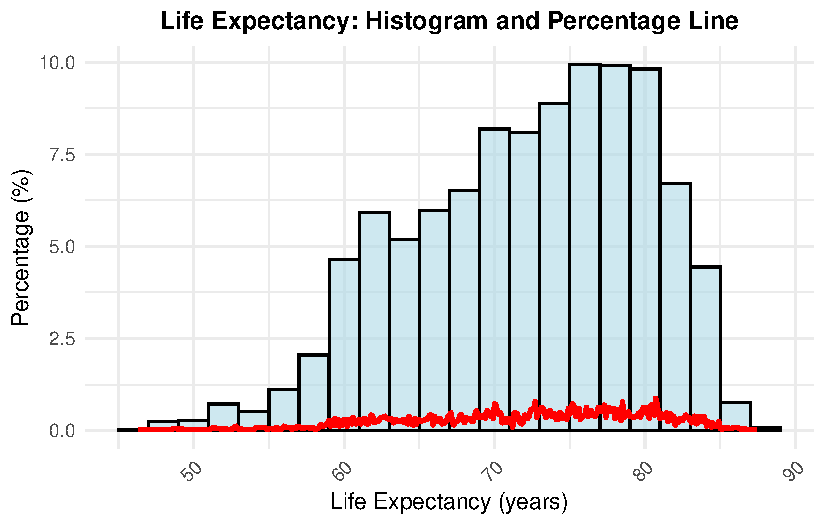
\includegraphics{paper_files/figure-pdf/fig-expectancy-1.pdf}

}

\caption{\label{fig-expectancy}This histogram shows the distribution of
the percentage of life expectancy for all years. Among all the life
expectancy ranges, 76-81 has the largest percenage of 24.7\%, while the
46-51 has the 0.54\%. Life expectancy shows a growing trend with the
increasing of age and drop sharply comes to the 81-86 range.}

\end{figure}%

\subsection{Predictor Variables}\label{predictor-variables}

The \textbf{predictor variables} (or independent variables) are the
factors believed to influence the life expectancy:

\begin{enumerate}
\def\labelenumi{\arabic{enumi}.}
\tightlist
\item
  \textbf{Income Group(\texttt{Income\_Group})}: The income group of a
  country is the key factor influencing the life expectancy. This
  variable provides context for comparing life expectancy between
  different levels of country income group. The division of the life
  expectancy by the income group of a country because income levels
  often correlate strongly with various factors affecting health and
  longevity. Higher income countries typically have more resources to
  invest in robust healthcare systems, with better living conditions
  while lower income countries often face challenges such as inadequate
  healthcare infrastructure and malnutrition.
\end{enumerate}

Following by the four income group, we would like to see the
distribution of the income group of 184 WHO member countries.
(\textbf{fid-income?}) shows that there are 55 countries at the high
income group, 26 countries at low income group, 54 countries at the
lower-middle group while there are 49 countries at the upper-middle
group. With significant less low income countries, we expect to see the
life expectancy lie in a comparably higher range. On the other hand,
there might exist sever outliers dropping the mean.

\begin{enumerate}
\def\labelenumi{\arabic{enumi}.}
\setcounter{enumi}{1}
\item
  \textbf{Gender(\texttt{Gender})}: The gender of the population of each
  country is included as a categorical variable (Male/Female/Both Sex).
  This is a key variable in the dataset because gender has been fully
  recognized connected with the biological physical factor which
  directly effect the life expectancy. Figure~\ref{fig-gender} shows
  that the with an stable average of 74, life expectancy of female is
  constantly higher than male's average of 70. The line plot reveals a
  steady increase until 2019, followed by a sharp decline in 2020, which
  is assumed to be associated with the impact of COVID-19.
\item
  \textbf{Region(Region)}: This is a categorical variable that
  classifies the geographic location of the countries. It is mapped one
  by one by the name of the country. The data is stored as the name of
  the continent(`Africa', `Oceania', `Asia', `Europe', `North America',
  `South America'). Figure~\ref{fig-region} indicates that with the
  number of 54, Africa has the most WHO member countries. Both Asia and
  Europe has 43 countries,listing in the middle while the other three
  continent has the significant less number of countries. North America
  has 22 countries, South America has 12 countries and Oceania has the
  least, 10 countries.
\end{enumerate}

\begin{figure}

\centering{

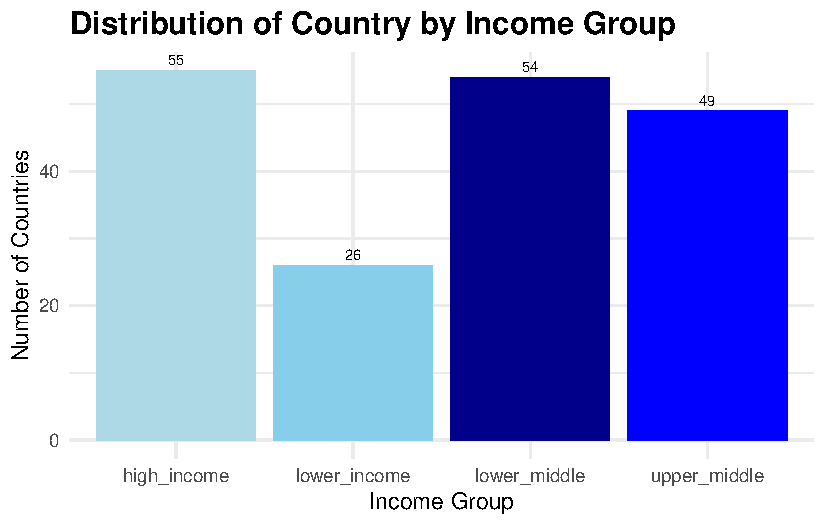
\includegraphics{paper_files/figure-pdf/fig-income-1.pdf}

}

\caption{\label{fig-income}Distribution of country income group.}

\end{figure}%

\begin{figure}

\centering{

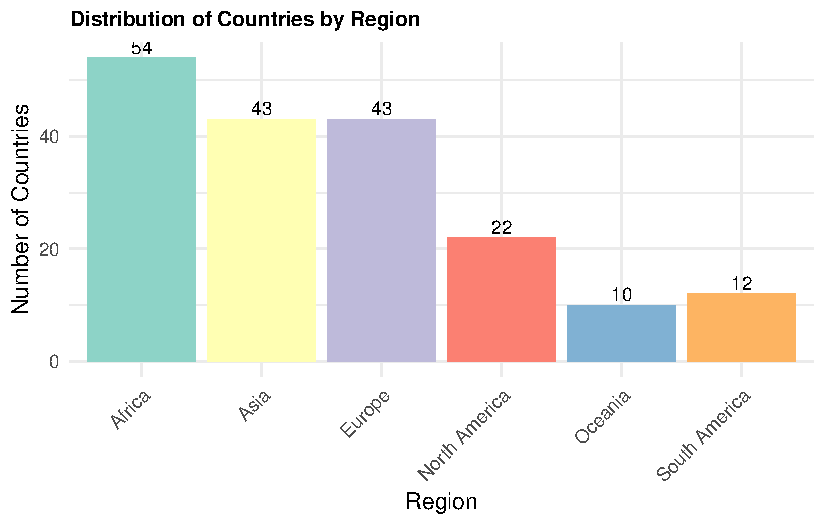
\includegraphics{paper_files/figure-pdf/fig-region-1.pdf}

}

\caption{\label{fig-region}Distribution of different region of the 184
countries. Africa has the most countries with an number of 54. Asia and
Europe has the same amount of 43, North America has 22 countries while
the other two continent has almost the same amount of countries.}

\end{figure}%

\begin{figure}

\centering{

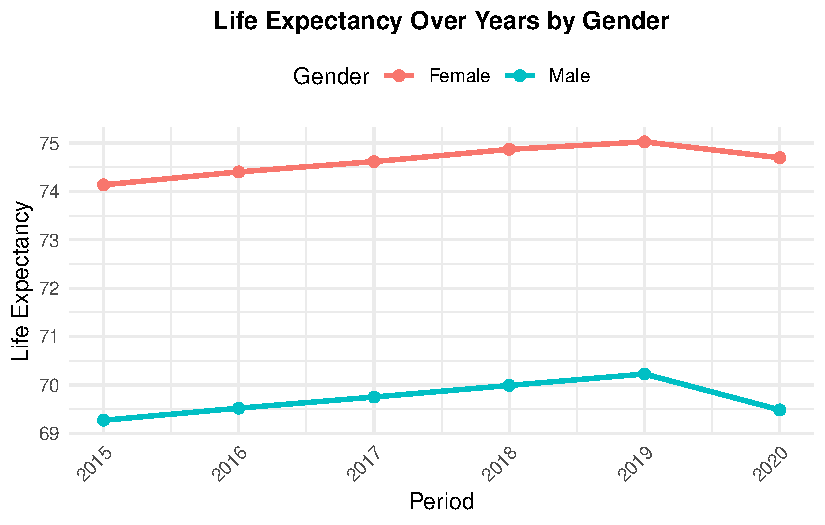
\includegraphics{paper_files/figure-pdf/fig-gender-1.pdf}

}

\caption{\label{fig-gender}Distribution of gender each year. The average
of female life expectancy is approximately 74 around years, constantly
higher than male's average of 70. Compared to male, female's life
expectancy is marginally more steady.}

\end{figure}%

\subsection{Basic Data Summary}\label{basic-data-summary}

The table below shows the basic summary of the mean, median, max,
standard deviation, variance and sample size of life expectancy. We
could tell that the average of the life expectancy from the 6 years is
72.2, with a relatively small standard deviation of 7.8. The max of the
life expectancy is 87.4, among all 3312 rows of data. The variance is
high because of the range of data is large, in other words, because the
mean and median are 72.2 and 73.1, compared to the max 87.4, there is
likely some outliers in the data creating such a slightly high variance
of 60.1.

\begin{figure}

\centering{

\begin{table}
\centering
\caption{Summary Statistics of Life Expectancy}
\centering
\fontsize{14}{16}\selectfont
\begin{tabular}[t]{>{}c|>{}c|>{}c|>{}c|>{}c|>{}c}
\hline
\multicolumn{6}{c}{ } \\

\cellcolor{lightgray}{\textbf{Mean}} & \cellcolor{lightgray}{\textbf{Median}} & \cellcolor{lightgray}{\textbf{Max}} & \cellcolor{lightgray}{\textbf{Standard Deviation}} & \cellcolor{lightgray}{\textbf{Variance}} & \cellcolor{lightgray}{\textbf{N}}\\
\hline
\cellcolor{darkblue}{\textcolor{white}{\textbf{72.2}}} & \textcolor{black}{73.1} & \textcolor{black}{87.4} & \textcolor{black}{7.8} & \textcolor{black}{60.1} & \textcolor{black}{3312}\\
\hline
\multicolumn{6}{l}{\rule{0pt}{1em}\textit{Note:} This table summarizes the key statistics of life expectancy data.}\\
\end{tabular}
\end{table}

}

\caption{\label{fig-summary}Summary statistics of the number of life
expectancy over countries and years.}

\end{figure}%

\section{Model}\label{model}

\subsection{Model set-up}\label{sec-modset}

The goal of the Bayesian model is to incorporate prior knowledge, such
as insights from previous studies or analyses, into the selection of the
model. To predict the outcome of the life expectancy of people from
different regions, in this paper, we developed a linear regression
models using R (R Core Team 2023). The outcome variable,
\textbf{\texttt{Life\ Expectancy}}, is a continuous and represents the
average number of years a person is expected to live, assuming all
related resources remain constant throughout their lifetime. The model
aim to estimate and predict the life expectancy of people under
different gender, region and income group. The normal Gaussian
distribution is effective when used for modeling scenarios where the
residuals of the data are assumed to be independent nd normally
distributed around the regression line. The GAM allows for capturing
potential non-linear relationships between the predictors and the
outcome.

The model is specified as follows:

\begin{align} 
y_i|\mu_i, \sigma &\sim \text{Normal}(\mu_i, \sigma) \text{(1)} \\
\mu_i &= \alpha + \beta_1 \text{Region}_i + \beta_2 \text{Gender}_i + \beta_3 \text{Income_Group}_i \\text{(2)} \\
\alpha &\sim \text{Normal}(0, 2.5) \text{(3)}\\
\beta_1, \beta_2, \beta_3 &\sim \text{Normal}(0, 2.5) \text{(4)}\\
\sigma &\sim \text{Exponential}(1) \text{(5)} \\
\end{align}

Where:

\begin{itemize}
\item
  \(yi\) is the outcome variable (Life Expectancy)for the i-th
  observation.
\item
  \(\mu_i\): the linear predictor for life expectancy, including the
  intercept (\(\alpha\)) and the coefficients for the predictors Region,
  Country, Income Group, and Gender.
\item
  Priors for the intercept(\(\alpha\)) and the
  coefficients(\(\beta_1, \beta_2, \beta_3\)) are normal with mean 0 and
  standard deviation 2.5
\item
  \(\sigma\): the residual standard deviation, modeled as an exponential
  distribution with rate 1.
\end{itemize}

We run the model in R (R Core Team 2023) using the \texttt{rstanarm}
package of Goodrich et al. (2022). We use the default priors from
\texttt{rstanarm}. More explanation of the model could be found
Appendix~\ref{sec-model-details}.

\subsubsection{Model justification}\label{model-justification}

The linear regression model with Gaussian likelihood was chosen for this
analysis due to its simplicity and effectiveness in modeling continuous
outcome variables, such as life expectancy. Life expectancy is
influenced by multiple factors, including region, income group, and
gender. The linear model allows us to examine the average effect of each
predictor on the outcome, assuming that the relationships between these
predictors and life expectancy are linear.

The use of normal priors for the model coefficients \(\alpha\) and
\(\beta\) reflects a belief in prior knowledge that the true values of
these parameters are centered around zero, with some uncertainty, which
is consistent with standard Bayesian modeling practices. The prior scale
of 2.5 was chosen to reflect a reasonable level of uncertainty around
the estimates without being overly restrictive.

The Gaussian distribution was selected because life expectancy data, by
nature, is continuous and expected to follow a normal distribution. The
assumption of normal residuals is consistent with the idea that
deviations from the regression line are random and normally distributed,
allowing the model to make accurate inferences about the relationship
between predictors and the outcome.

Additionally, the exponential prior on the standard deviation \(\alpha\)
captures the residual variability in life expectancy across countries
and regions. The exponential distribution was chosen because it provides
a simple and interpretable way of modeling the variability, assuming
that the data are not heavily skewed.

This approach is appropriate given the data structure and the goal of
the analysis, which is to estimate and predict life expectancy across
different countries, regions, income groups, and genders. The model's
assumptions about the data, along with its priors, allow for robust
inference in the context of population health predictions.

\paragraph{Model Validation}\label{model-validation}

To assess the performance of the life expectancy prediction model, two
critical metrics were used: Root Mean Squared Error (RMSE) and
Out-of-Sample Testing. These methods help ensure that the model
generalizes well to unseen data and provides reliable predictions for
life expectancy across different regions, income groups, and genders.

RMSE measures the square root of the average squared differences between
the predicted and observed values. In the context of this model, RMSE
quantifies how closely the predicted life expectancy values align with
the actual observed values. Lower RMSE values indicate better model
performance, suggesting that the model's predictions are close to the
true values. Table~\ref{tbl-modelpredict} gives out the RMSE of both
testing data and training data. The generalizability is checked by
comparing rmse\_test and rmse\_train. Seeing the test RMSE is slightly
lower than the training RMSE, the model generalizes well.

Out-of-Sample testing is a critical component of model evaluation. In
this approach, the data is split into a training set and a test set (or
holdout set). The training set is used to fit the model, while the test
set is used to evaluate how well the model performs on new, unseen data.
For this analysis, the model was trained using a portion of the data
(80\% of the dataset) and then evaluated on the remaining data (20\% of
the dataset) that was not used during training. This method allows us to
check whether the model overfits the training data or if it can
generalize well to unseen observations.

Together, RMSE and out-of-sample testing offer a robust framework for
model validation, ensuring that the predictions made by the life
expectancy model are both accurate and generalizable.

Extended versions of the table can be found in
Table~\ref{tbl-testpredicted}.

\begin{Shaded}
\begin{Highlighting}[]
\CommentTok{\# Split the dataset into training and testing sets (80\% train, 20\% test)}
\FunctionTok{set.seed}\NormalTok{(}\DecValTok{123}\NormalTok{)  }\CommentTok{\# Setting seed for reproducibility}
\NormalTok{train\_index }\OtherTok{\textless{}{-}} \FunctionTok{createDataPartition}\NormalTok{(leab}\SpecialCharTok{$}\StringTok{\textasciigrave{}}\AttributeTok{Life Expectancy}\StringTok{\textasciigrave{}}\NormalTok{, }\AttributeTok{p =} \FloatTok{0.8}\NormalTok{, }\AttributeTok{list =} \ConstantTok{FALSE}\NormalTok{)}

\NormalTok{train\_data }\OtherTok{\textless{}{-}}\NormalTok{ leab[train\_index, ]}
\NormalTok{test\_data }\OtherTok{\textless{}{-}}\NormalTok{ leab[}\SpecialCharTok{{-}}\NormalTok{train\_index, ]}

\CommentTok{\# Predict life expectancy using the test data}
\NormalTok{predictions }\OtherTok{\textless{}{-}} \FunctionTok{predict}\NormalTok{(model\_developed, }\AttributeTok{newdata =}\NormalTok{ test\_data)}
\end{Highlighting}
\end{Shaded}

\begin{table}

\caption{\label{tbl-modelpredict}Summary of the life expectancy model,
which includes gender, region and income group. The table presents the
model RSME and out-of sample testing.}

\centering{

\centering
\caption{RMSE Comparison for Test and Training Data}
\centering
\fontsize{14}{16}\selectfont
\begin{tabular}[t]{>{}c|>{}c}
\hline
\multicolumn{1}{c|}{ } & \multicolumn{1}{c}{Root Mean Squared Error (RMSE)} \\
\cline{2-2}
Dataset & RMSE\\
\hline
\cellcolor{steelblue}{\textcolor{white}{\textbf{Test Data}}} & \textcolor{black}{1.15}\\
\hline
\cellcolor{steelblue}{\textcolor{white}{\textbf{Training Data}}} & \textcolor{black}{1.17}\\
\hline
\end{tabular}

}

\end{table}%

\section{Results}\label{results}

\subsection{Data results analysis}\label{data-results-analysis}

According to the Table~\ref{tbl-sum_sta}, we could tell that

\subsection{Overview of model results}\label{overview-of-model-results}

Our results are summarized in Table~\ref{tbl-model}. We are primarily
interest in the general life expectancy regarding to the related
predictors. The multiple linear model provides us with the estimates for
the intercept and coefficients for the predictors which are male,
female, both genders, lower income, lower-middle, upper-middle, high
income, Asia, Europe, Africa, Oceania, North America and South America.
The intercept represents the estimate of region-standard life expectancy
when all the predictors are zero. The coefficients represent the
additional life expectancy associated with each predictor. The model
results will display the estimates- posterior means or medians for each
coefficient including the intercept, uncertainty measures- credible
intervals. The output values of each predictor is the regression
coefficient, meaning how much the outcome is expected to increase or
decrease with one unit increase in the life expectancy (per year) of
that predictor, holding all else constant. The value in the brackets
represent the Median Absolute Deviation of the posterior distributions
of the coefficients. It conveys the dispersion around the median of each
coefficients' posterior distribution, exhibiting how spread the
distributions are.

Num.Obs represents the number of observations made in the model. R2 is
the R-squared value which is the proportion of variance in the dependent
variable that can be explained bu the independent variable. The R2 adj
is the adjusted R squared which accounts for the number of predictors
used. Log.lik is the log-likelihood which gives us an idea of the
likelihood of the data, higher is the better, but this is typically used
for comparison between the models. ELPD and ELPD s.e. explains the log
predictive density and its standard error. The ELPD measures the sum of
the log predictive densities for each observation, used for model
comparison. LOOIC is an acronym for leave-one-out information criterion
in which a lower value indicates a model with better out-of-sample
predictive performance. WAIC stands for Watanabe-Akaike information
criterion which is another measure of good fit; lower values are better
fit. RMSE is the room mean squared error measuring the models's
predictive performance where lower values means more accurate predicts.

\begin{table}

\caption{\label{tbl-model}Summary of the life expectancy model, which
includes gender, region and income group. The table presents the model
RSME and out-of sample testing.}

\centering{

\centering
\begin{tblr}[         %% tabularray outer open
]                     %% tabularray outer close
{                     %% tabularray inner open
colspec={Q[]Q[]},
column{1}={halign=l,},
column{2}={halign=c,},
hline{390}={1,2}{solid, 0.05em, black},
}                     %% tabularray inner close
\toprule
& Gaussian(Normal) \\ \midrule %% TinyTableHeader
(Intercept)                                                 & \num{79.53}     \\
& (\num{43.50})   \\
RegionAsia                                                  & \num{-6.22}     \\
& (\num{21.20})   \\
RegionEurope                                                & \num{-8.39}     \\
& (\num{45.65})   \\
RegionNorth America                                         & \num{-5.48}     \\
& (\num{50.68})   \\
RegionOceania                                               & \num{-8.43}     \\
& (\num{80.66})   \\
RegionSouth America                                         & \num{21.91}     \\
& (\num{55.21})   \\
CountryAlbania                                              & \num{0.68}      \\
& (\num{28.99})   \\
CountryAlgeria                                              & \num{9.41}      \\
& (\num{47.74})   \\
CountryAngola                                               & \num{-4.60}     \\
& (\num{47.88})   \\
CountryAntigua and Barbuda                                  & \num{2.12}      \\
& (\num{31.15})   \\
CountryArgentina                                            & \num{-28.26}    \\
& (\num{65.45})   \\
CountryArmenia                                              & \num{-3.20}     \\
& (\num{29.08})   \\
CountryAustralia                                            & \num{17.28}     \\
& (\num{64.59})   \\
CountryAustria                                              & \num{7.63}      \\
& (\num{26.97})   \\
CountryAzerbaijan                                           & \num{-2.97}     \\
& (\num{29.29})   \\
CountryBahamas                                              & \num{-1.15}     \\
& (\num{31.29})   \\
CountryBahrain                                              & \num{3.35}      \\
& (\num{36.83})   \\
CountryBangladesh                                           & \num{4.23}      \\
& (\num{54.21})   \\
CountryBarbados                                             & \num{2.55}      \\
& (\num{30.97})   \\
CountryBelarus                                              & \num{-3.11}     \\
& (\num{29.12})   \\
CountryBelgium                                              & \num{7.36}      \\
& (\num{26.87})   \\
CountryBelize                                               & \num{0.25}      \\
& (\num{30.40})   \\
CountryBenin                                                & \num{-3.17}     \\
& (\num{48.20})   \\
CountryBhutan                                               & \num{4.36}      \\
& (\num{54.23})   \\
CountryBolivia (Plurinational State of)                     & \num{-24.08}    \\
& (\num{76.01})   \\
CountryBosnia and Herzegovina                               & \num{-0.20}     \\
& (\num{29.18})   \\
CountryBotswana                                             & \num{-19.85}    \\
& (\num{51.26})   \\
CountryBrazil                                               & \num{-30.04}    \\
& (\num{65.42})   \\
CountryBrunei Darussalam                                    & \num{4.00}      \\
& (\num{36.91})   \\
CountryBulgaria                                             & \num{-2.45}     \\
& (\num{29.09})   \\
CountryBurkina Faso                                         & \num{-5.08}     \\
& (\num{21.33})   \\
CountryBurundi                                              & \num{-3.23}     \\
& (\num{21.40})   \\
CountryCabo Verde                                           & \num{7.65}      \\
& (\num{47.94})   \\
CountryCambodia                                             & \num{-0.02}     \\
& (\num{54.13})   \\
CountryCameroon                                             & \num{-5.86}     \\
& (\num{48.02})   \\
CountryCanada                                               & \num{7.86}      \\
& (\num{30.96})   \\
CountryCentral African Republic                             & \num{-14.92}    \\
& (\num{21.25})   \\
CountryChad                                                 & \num{-8.32}     \\
& (\num{21.18})   \\
CountryChile                                                & \num{-24.65}    \\
& (\num{56.84})   \\
CountryChina                                                & \num{-4.35}     \\
& (\num{51.31})   \\
CountryColombia                                             & \num{-27.30}    \\
& (\num{65.38})   \\
CountryComoros                                              & \num{1.26}      \\
& (\num{48.11})   \\
CountryCongo                                                & \num{-3.93}     \\
& (\num{48.00})   \\
CountryCosta Rica                                           & \num{5.85}      \\
& (\num{30.49})   \\
CountryCote d'Ivoire                                        & \num{-4.15}     \\
& (\num{48.20})   \\
CountryCroatia                                              & \num{4.47}      \\
& (\num{26.98})   \\
CountryCuba                                                 & \num{3.41}      \\
& (\num{30.53})   \\
CountryCyprus                                               & \num{8.31}      \\
& (\num{26.83})   \\
CountryCzechia                                              & \num{5.01}      \\
& (\num{27.04})   \\
CountryDemocratic People's Republic of Korea                & \num{11.23}     \\
& (\num{0.48})    \\
CountryDemocratic Republic of the Congo                     & \num{-5.91}     \\
& (\num{21.28})   \\
CountryDenmark                                              & \num{7.40}      \\
& (\num{26.95})   \\
CountryDjibouti                                             & \num{-1.98}     \\
& (\num{47.97})   \\
CountryDominican Republic                                   & \num{-0.78}     \\
& (\num{30.48})   \\
CountryEcuador                                              & \num{-28.26}    \\
& (\num{65.51})   \\
CountryEgypt                                                & \num{4.21}      \\
& (\num{47.84})   \\
CountryEl Salvador                                          & \num{-0.99}     \\
& (\num{30.48})   \\
CountryEquatorial Guinea                                    & \num{-22.60}    \\
& (\num{51.41})   \\
CountryEritrea                                              & \num{-3.74}     \\
& (\num{21.28})   \\
CountryEstonia                                              & \num{4.46}      \\
& (\num{26.91})   \\
CountryEswatini                                             & \num{-12.28}    \\
& (\num{48.03})   \\
CountryEthiopia                                             & \num{1.13}      \\
& (\num{21.26})   \\
CountryFiji                                                 & \num{-0.68}     \\
& (\num{71.02})   \\
CountryFinland                                              & \num{7.61}      \\
& (\num{27.08})   \\
CountryFrance                                               & \num{8.48}      \\
& (\num{26.98})   \\
CountryGabon                                                & \num{-19.19}    \\
& (\num{51.46})   \\
CountryGambia                                               & \num{-2.56}     \\
& (\num{21.32})   \\
CountryGeorgia                                              & \num{-3.87}     \\
& (\num{29.20})   \\
CountryGermany                                              & \num{7.02}      \\
& (\num{27.00})   \\
CountryGhana                                                & \num{-1.35}     \\
& (\num{47.86})   \\
CountryGreece                                               & \num{7.16}      \\
& (\num{26.98})   \\
CountryGrenada                                              & \num{-1.25}     \\
& (\num{30.43})   \\
CountryGuatemala                                            & \num{-2.17}     \\
& (\num{30.39})   \\
CountryGuinea                                               & \num{-6.20}     \\
& (\num{47.88})   \\
CountryGuinea-Bissau                                        & \num{-8.80}     \\
& (\num{21.23})   \\
CountryGuyana                                               & \num{-37.07}    \\
& (\num{56.78})   \\
CountryHaiti                                                & \num{-1.41}     \\
& (\num{33.25})   \\
CountryHonduras                                             & \num{6.26}      \\
& (\num{33.17})   \\
CountryHungary                                              & \num{2.27}      \\
& (\num{27.02})   \\
CountryIceland                                              & \num{8.69}      \\
& (\num{26.93})   \\
CountryIndia                                                & \num{1.11}      \\
& (\num{54.41})   \\
CountryIndonesia                                            & \num{-10.63}    \\
& (\num{51.36})   \\
CountryIran (Islamic Republic of)                           & \num{7.86}      \\
& (\num{54.06})   \\
CountryIraq                                                 & \num{-9.81}     \\
& (\num{51.25})   \\
CountryIreland                                              & \num{8.03}      \\
& (\num{26.93})   \\
CountryIsrael                                               & \num{9.91}      \\
& (\num{36.89})   \\
CountryItaly                                                & \num{8.81}      \\
& (\num{26.91})   \\
CountryJamaica                                              & \num{-1.99}     \\
& (\num{30.43})   \\
CountryJapan                                                & \num{11.94}     \\
& (\num{36.88})   \\
CountryJordan                                               & \num{9.67}      \\
& (\num{54.24})   \\
CountryKazakhstan                                           & \num{-4.71}     \\
& (\num{29.26})   \\
CountryKenya                                                & \num{-0.86}     \\
& (\num{47.87})   \\
CountryKiribati                                             & \num{4.08}      \\
& (\num{61.70})   \\
CountryKuwait                                               & \num{9.87}      \\
& (\num{36.84})   \\
CountryKyrgyzstan                                           & \num{3.47}      \\
& (\num{54.41})   \\
CountryLao People's Democratic Republic                     & \num{-1.48}     \\
& (\num{54.13})   \\
CountryLatvia                                               & \num{1.45}      \\
& (\num{26.95})   \\
CountryLebanon                                              & \num{9.14}      \\
& (\num{54.11})   \\
CountryLesotho                                              & \num{-15.82}    \\
& (\num{48.08})   \\
CountryLiberia                                              & \num{-4.50}     \\
& (\num{21.35})   \\
CountryLibya                                                & \num{-10.87}    \\
& (\num{51.31})   \\
CountryLithuania                                            & \num{1.52}      \\
& (\num{27.02})   \\
CountryLuxembourg                                           & \num{9.05}      \\
& (\num{26.98})   \\
CountryMadagascar                                           & \num{-3.54}     \\
& (\num{21.21})   \\
CountryMalawi                                               & \num{-4.38}     \\
& (\num{21.25})   \\
CountryMalaysia                                             & \num{-6.51}     \\
& (\num{51.20})   \\
CountryMaldives                                             & \num{-4.14}     \\
& (\num{51.20})   \\
CountryMali                                                 & \num{-6.00}     \\
& (\num{21.21})   \\
CountryMalta                                                & \num{8.28}      \\
& (\num{26.88})   \\
CountryMauritania                                           & \num{2.98}      \\
& (\num{47.95})   \\
CountryMauritius                                            & \num{-9.94}     \\
& (\num{51.30})   \\
CountryMexico                                               & \num{0.67}      \\
& (\num{30.33})   \\
CountryMicronesia (Federated States of)                     & \num{8.09}      \\
& (\num{61.64})   \\
CountryMongolia                                             & \num{1.06}      \\
& (\num{54.16})   \\
CountryMontenegro                                           & \num{-0.28}     \\
& (\num{29.22})   \\
CountryMorocco                                              & \num{6.69}      \\
& (\num{48.03})   \\
CountryMozambique                                           & \num{-9.56}     \\
& (\num{21.26})   \\
CountryMyanmar                                              & \num{-0.94}     \\
& (\num{54.36})   \\
CountryNamibia                                              & \num{-21.00}    \\
& (\num{51.42})   \\
CountryNepal                                                & \num{1.41}      \\
& (\num{54.14})   \\
CountryNetherlands (Kingdom of the)                         & \num{8.02}      \\
& (\num{27.04})   \\
CountryNew Zealand                                          & \num{16.32}     \\
& (\num{64.57})   \\
CountryNicaragua                                            & \num{13.32}     \\
& (\num{33.40})   \\
CountryNiger                                                & \num{-6.88}     \\
& (\num{21.20})   \\
CountryNigeria                                              & \num{-4.28}     \\
& (\num{48.05})   \\
CountryNorth Macedonia                                      & \num{-1.40}     \\
& (\num{29.34})   \\
CountryNorway                                               & \num{8.78}      \\
& (\num{26.93})   \\
CountryOman                                                 & \num{2.38}      \\
& (\num{36.87})   \\
CountryPakistan                                             & \num{-3.13}     \\
& (\num{54.28})   \\
CountryPanama                                               & \num{4.48}      \\
& (\num{31.13})   \\
CountryPapua New Guinea                                     & \num{8.94}      \\
& (\num{61.59})   \\
CountryParaguay                                             & \num{-29.48}    \\
& (\num{65.36})   \\
CountryPeru                                                 & \num{-26.42}    \\
& (\num{65.46})   \\
CountryPhilippines                                          & \num{0.30}      \\
& (\num{54.15})   \\
CountryPoland                                               & \num{3.67}      \\
& (\num{27.01})   \\
CountryPortugal                                             & \num{7.36}      \\
& (\num{27.07})   \\
CountryPuerto Rico                                          & \num{6.28}      \\
& (\num{31.19})   \\
CountryQatar                                                & \num{5.93}      \\
& (\num{36.80})   \\
CountryRepublic of Korea                                    & \num{10.61}     \\
& (\num{36.81})   \\
CountryRepublic of Moldova                                  & \num{-4.72}     \\
& (\num{29.13})   \\
CountryRomania                                              & \num{1.39}      \\
& (\num{26.96})   \\
CountryRussian Federation                                   & \num{-9.31}     \\
& (\num{51.36})   \\
CountryRwanda                                               & \num{0.44}      \\
& (\num{21.29})   \\
CountrySaint Lucia                                          & \num{1.72}      \\
& (\num{30.45})   \\
CountrySaint Vincent and the Grenadines                     & \num{-1.25}     \\
& (\num{30.38})   \\
CountrySamoa                                                & \num{12.64}     \\
& (\num{61.59})   \\
CountrySao Tome and Principe                                & \num{4.58}      \\
& (\num{47.96})   \\
CountrySaudi Arabia                                         & \num{4.35}      \\
& (\num{36.87})   \\
CountrySenegal                                              & \num{1.47}      \\
& (\num{48.01})   \\
CountrySerbia                                               & \num{-1.59}     \\
& (\num{29.20})   \\
CountrySeychelles                                           & \num{-5.53}     \\
& (\num{43.56})   \\
CountrySierra Leone                                         & \num{-7.75}     \\
& (\num{21.34})   \\
CountrySingapore                                            & \num{10.98}     \\
& (\num{36.89})   \\
CountrySlovakia                                             & \num{3.40}      \\
& (\num{27.00})   \\
CountrySlovenia                                             & \num{7.13}      \\
& (\num{27.00})   \\
CountrySolomon Islands                                      & \num{7.87}      \\
& (\num{61.68})   \\
CountrySomalia                                              & \num{-12.52}    \\
& (\num{21.30})   \\
CountrySouth Africa                                         & \num{-19.37}    \\
& (\num{51.43})   \\
CountrySouth Sudan                                          & \num{-8.01}     \\
& (\num{21.29})   \\
CountrySpain                                                & \num{8.85}      \\
& (\num{27.13})   \\
CountrySri Lanka                                            & \num{7.99}      \\
& (\num{54.25})   \\
CountrySudan                                                & \num{1.81}      \\
& (\num{21.31})   \\
CountrySuriname                                             & \num{-31.76}    \\
& (\num{65.41})   \\
CountrySweden                                               & \num{8.42}      \\
& (\num{26.97})   \\
CountrySwitzerland                                          & \num{9.33}      \\
& (\num{27.01})   \\
CountrySyrian Arab Republic                                 & \num{3.97}      \\
& (\num{0.40})    \\
CountryTajikistan                                           & \num{3.09}      \\
& (\num{53.97})   \\
CountryThailand                                             & \num{-4.50}     \\
& (\num{51.28})   \\
CountryTimor-Leste                                          & \num{-0.90}     \\
& (\num{54.22})   \\
CountryTogo                                                 & \num{-4.19}     \\
& (\num{21.21})   \\
CountryTonga                                                & \num{4.42}      \\
& (\num{71.06})   \\
CountryTrinidad and Tobago                                  & \num{0.20}      \\
& (\num{31.16})   \\
CountryTunisia                                              & \num{10.40}     \\
& (\num{47.95})   \\
CountryTürkiye                                              & \num{-4.47}     \\
& (\num{51.31})   \\
CountryTurkmenistan                                         & \num{-12.58}    \\
& (\num{51.24})   \\
CountryUganda                                               & \num{-1.74}     \\
& (\num{21.23})   \\
CountryUkraine                                              & \num{6.68}      \\
& (\num{36.36})   \\
CountryUnited Arab Emirates                                 & \num{8.68}      \\
& (\num{36.79})   \\
CountryUnited Kingdom of Great Britain and Northern Ireland & \num{7.08}      \\
& (\num{27.10})   \\
CountryUnited Republic of Tanzania                          & \num{-0.45}     \\
& (\num{47.88})   \\
CountryUnited States of America                             & \num{4.57}      \\
& (\num{31.22})   \\
CountryUruguay                                              & \num{-27.80}    \\
& (\num{56.83})   \\
CountryUzbekistan                                           & \num{1.65}      \\
& (\num{54.36})   \\
CountryVanuatu                                              & \num{9.66}      \\
& (\num{61.72})   \\
CountryVenezuela (Bolivarian Republic of)                   & \num{-31.90}    \\
& (\num{65.65})   \\
CountryViet Nam                                             & \num{3.94}      \\
& (\num{53.92})   \\
CountryYemen                                                & \num{6.61}      \\
& (\num{0.40})    \\
CountryZambia                                               & \num{-5.46}     \\
& (\num{47.98})   \\
CountryZimbabwe                                             & \num{-8.25}     \\
& (\num{48.08})   \\
Income\_Grouplower\_income                                & \num{-12.06}    \\
& (\num{36.90})   \\
Income\_Grouplower\_middle                                & \num{-4.04}     \\
& (\num{23.94})   \\
Income\_Groupupper\_middle                                & \num{3.40}      \\
& (\num{20.47})   \\
GenderFemale                                                & \num{2.50}      \\
& (\num{0.05})    \\
GenderMale                                                  & \num{-2.42}     \\
& (\num{0.05})    \\
Num.Obs.                                                    & \num{3312}      \\
R2                                                          & \num{0.976}     \\
R2 Adj.                                                     & \num{0.975}     \\
Log.Lik.                                                    & \num{-5231.038} \\
ELPD                                                        & \num{-5409.7}   \\
ELPD s.e.                                                   & \num{94.5}      \\
LOOIC                                                       & \num{10819.4}   \\
LOOIC s.e.                                                  & \num{189.0}     \\
WAIC                                                        & \num{10816.6}   \\
RMSE                                                        & \num{4.37}      \\
\bottomrule
\end{tblr}

}

\end{table}%

\subsection{Multiple linear regression
results}\label{multiple-linear-regression-results}

Table~\ref{tbl-model} is thye table of the results from out model.

\section{Discussion}\label{discussion}

\subsection{Insights into Life Expectancy Differences by
Gender}\label{insights-into-life-expectancy-differences-by-gender}

Thought the result part we have noticed that female constantly have
higher life expectancy than male. Figure~\ref{fig-gender} shows that
female has around 4 years higher average age than male. Even during the
sudden drop of 2020, female kept a more stable trend than male. Through
literature research, we found that historically women tend to have
longer life than men across most regions and cultures.
(\textbf{whymandieyounger?})These difference can be attributed to a
variety of interconnected reasons. Women generally have stronger immune
systems and are less prone to certain life-threatening diseases like
cardiovascular diseases in early adulthood. Estrogen, a hormone
prevalent in women, provides some protection against heart disease by
improving cholesterol levels. On the other hand, men are more prone to
risk factors such as hypertension and higher levels of LDL cholesterol,
which contribute to shorter life spansehavioral patterns
(\textbf{behaviouralfactor?}). What's more, male are more likely to
engage in behaviours such as smoking, excessive alcohol consumption and
hazardous occupations. These behaviors increase the risk of accidents,
chronic diseases, and early mortality. Last but not least, globally,
women tend to use healthcare services more frequently than men, which
allows for earlier detection and treatment of illnesses. Men often delay
seeking medical care, worsening outcomes for preventable or manageable
diseases.(\textbf{womenhigherhealthcare?})

\subsection{Insights into Life Expectancy Differences by Income
Group}\label{insights-into-life-expectancy-differences-by-income-group}

From the summary and analysis of \textbf{?@tbl-regresult}, we have seen
that high income group has the significant high life expectancy compared
to the lower income group, which indicates that life expectancy is
significantly influenced by income groups. It is known that income
determines access to resources, healthcare and living conditions.
Difference in life expectancy across income groups reflect broader
inequalities in socioeconomic factors and highlight disparities in
global health outcomes.

High-income groups have greater access to quality healthcare services,
including preventive care, advanced medical treatments, and regular
health checkups.Conversely, lower-income groups often face barriers such
as cost, lack of infrastructure, and insufficient health insurance
coverage, leading to untreated or poorly managed health conditions
(\textbf{inequalworld?}). Other living conditions like access to
nutritious food, safe drinking water and sanitary living environments
are also linked with high economics. Low-income populations are more
likely to experience malnutrition, exposure to environmental toxins, and
overcrowded living conditions, all of which negatively impact health and
life expectancy.

What's more, lower-income individuals are often exposed to higher levels
of chronic stress due to financial instability and job insecurity.
Stress is linked to adverse health outcomes such as hypertension,
cardiovascular diseases, and mental health issues
(\textbf{incomeinequality?}). Moreover, low-income workers frequently
engage in physically demanding or hazardous jobs, increasing their risk
of injury and illness. All these factors together makes the lower income
countries disadvantage in life expectancy.

\subsection{Life Expectancy at 60}\label{life-expectancy-at-60}

The life expectancy at 60 means that how long is a person expected to
live at 60 instead of at birth. From the box plot
Figure~\ref{fig-lea60}, we could tell the high-income group tends to
have an average life expectancy of approximately 23 years at age 60,
whereas the lower-income group averages around 16 years. Notably, the
lower-middle-income group exhibits the largest variance, with the most
outliers, indicating a wide disparity in life expectancy within this
category.

The data also reveal a clear trend: as income levels increase, so does
the average life expectancy at age 60. This aligns with findings from
analyses of life expectancy at birth, emphasizing the significant
correlation between income and life expectancy. Higher-income groups
likely benefit from better access to healthcare, nutrition, and living
conditions, which collectively contribute to improved longevity.

Life expectancy at 60 provides insights into the additional years a
person can expect to live after reaching 60, reflecting the health and
living conditions of older populations. Unlike life expectancy at birth,
which captures the average years a newborn is expected to live based on
current mortality rates across all ages, life expectancy at 60 excludes
the impact of child and early-adult mortality. This makes it
particularly useful for assessing health outcomes, chronic disease
management, and the effectiveness of healthcare systems for aging
populations. It highlights longevity and quality of life in later years,
crucial for designing age-focused policies and support systems.

\begin{figure}

\centering{

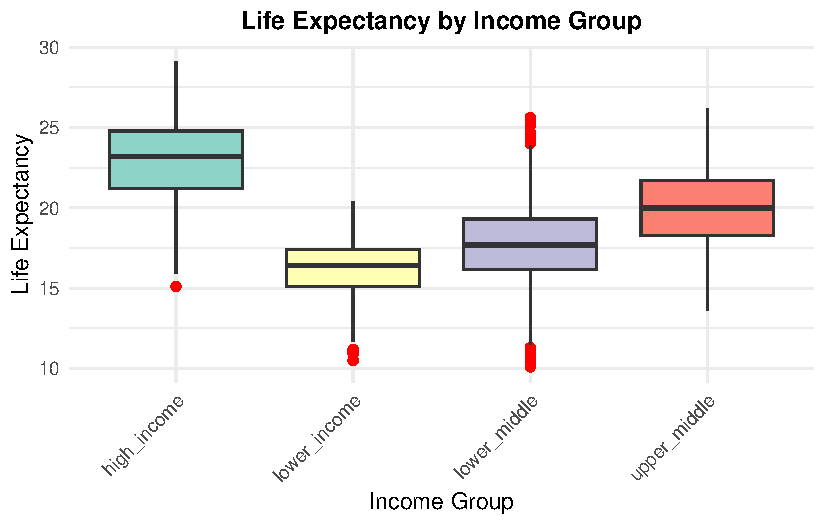
\includegraphics{paper_files/figure-pdf/fig-lea60-1.pdf}

}

\caption{\label{fig-lea60}Box plot of life expectancy at 60 by different
income group. The high income group tend to have 23 years of life
expectancy at 60 while the lower income group has an average of 16 years
at 60. It is noticable that lower middle has the most outlier showing
the largest varaiance.}

\end{figure}%

\subsection{Weaknesses and next steps}\label{weaknesses-and-next-steps}

\subsubsection{Other factors related to income group and
region}\label{other-factors-related-to-income-group-and-region}

Income groups, often categorized as low, middle, or high-income, play a
significant role in determining access to resources and opportunities
that directly and indirectly affect life expectancy. However, income
group classifications themselves are shaped by a variety of factors that
this analysis may not have accounted for, which introduces limitations
to the model. Region would be one key factor that influence the income
group. Regions with limited access to stable employment opportunities
may fall into lower-income groups, leading to reduced access to
healthcare, education, and nutritious food, all of which affect life
expectancy. It is reckon that trade imbalances, resource exploitation,
and historical colonization have left some countries with weak economies
and infrastructure, directly influencing their classification as low or
middle-income. Since these factors influence the income groups, their
absence in the model creates a gap in understanding how income
ultimately impacts life expectancy. A comprehensive model should explore
these underlying determinants of income groups alongside traditional
predictors of life expectancy.

\subsubsection{Dataset limitation}\label{dataset-limitation}

Weakness may arise from the generalization of the data. When working
with data provided by authoritative sources like the World Health
Organization (WHO), it's important to recognize the methodological
nuances underlying the calculations. In this case, the dataset includes
average life expectancy values, which are themselves estimates derived
from sophisticated statistical and demographic models. The accuracy of
the derived averages depends heavily on the statistical methods used by
WHO. Since the initial dataset offers the average of the life expectancy
of each country which are calculated after several factor, these
assumptions cascade into our analysis. The ``average of averages''
cannot rectify inaccuracies or gaps in the original model.

By acknowledging these limitations and incorporating appropriate
statistical techniques, for further studies, it would be suggested to
use a more variety of models such as the multilevel modeling to increase
the accuracy of the model by cross validation or comparing the results
from other models as well. Study deeper into the correlations with more
factors we discussed above would let us notice which factors influences
life expectancy. Like mentioned in the introduction, this analysis aims
to empower policymakers by providing critical insights into factors
affecting life expectancy across various regions, genders, and income
groups. By addressing identified limitations and leveraging data-driven
strategies, analyses can better capture the complexities of life
expectancy data and provide insights that align more closely with
real-world dynamics while policymakers can implement targeted
interventions to improve healthcare access, reduce disparities, and
enhance the overall quality of life for their populations.

\newpage

\appendix

\section{Appendix}\label{sec-appendix}

\subsection{Data Cleaning Notes}\label{data-cleaning-notes}

We began by importing the raw dataset using the read\_csv function from
the tidyverse package. To focus our analysis on more relevant variables,
we selected specific columns, such as Indicator of life expectancy as
birth and life expectancy at 60 years, Country, Period, Gender, and Life
expectancy, omitting any unnecessary columns.

We functioned to extract the number before opening the square bracket of
life expectancy since the raw data gave both the range and the mean of
life expectancy of each country under each year.

We filter out the rows containing NA values in any of the selected
columns for reducing the noise and simpler further analysis.

We then renaming columns for clarity. For example, we changed `Location'
into `Country', ``Dim1'' for ``Gender'' and ``Value'' for ``Life
Expectancy'', making it easier for anyone working with the data to read
and understand what each variable represents.

Each column is rounded using the round function, specifying the desired
number of decimal places for each. Columns not mentioned in mutate
remain unchanged. This ensures a flexible and precise cleaning process
tailored to further comparison and graphing. We dropped the potential
percentage symbol to contain purely numerical data.

The income group column and the region column was not given in the raw
dataset. We created a new variable called ``Income\_Group'' by mapping
over country name to four income group (lower\_income, lower\_middle,
upper\_middle, high\_income) according to the index given by World Bank
Income Group. This is a key variable in predicting life expectancy since
it is believed that life expectancy is correlated to the income
situation. We as well made a mapping to the countries according to its
continent and saved as ``Region''. This is the variable indicates the
geographic context to the analysis. Countries are mapped into six
continents (``Africa'', ``Asia'', ``Europe'', ``North America'', ``South
America'', ``Oceania'') one by one.

We again merge the table, removing repeated columns and rows and mapping
the region and the country income under different given names.

Lastly, we filter out NAs again as a further check. We continue filter
out the Palestinian territory, which is not a country and was not mapped
in neither Region nor Income Group.

For easy reading format, we arrange the country into Alphabet order and
mutate the variables again for converting columns into appropriate data
types.

For easier visualization, we created four tables, which are grouped by
life expectancy at age 60, life expectancy at birth, life expectancy at
birth of Male and life expectancy at birth of Female.

After completing the cleaning, we saved the final dataset in both
Parquet and CSV formats for later analysis.

\subsection{Data Cleaning Full Table}\label{data-cleaning-full-table}

\begin{longtable}[t]{llll>{}r}

\caption{\label{tbl-cleaned_average}Full cleaned Average life
expectancy}

\tabularnewline

\toprule
\cellcolor[HTML]{0073C2}{\textcolor{white}{\textbf{Country}}} & \cellcolor[HTML]{0073C2}{\textcolor{white}{\textbf{Gender}}} & \cellcolor[HTML]{0073C2}{\textcolor{white}{\textbf{Income Group}}} & \cellcolor[HTML]{0073C2}{\textcolor{white}{\textbf{Region}}} & \cellcolor[HTML]{0073C2}{\textcolor{white}{\textbf{Average Life Expectancy}}}\\
\midrule
Afghanistan & Both sexes & lower\_income & Asia & \cellcolor[HTML]{F7F7F7}{\textbf{60.63}}\\
Afghanistan & Female & lower\_income & Asia & \cellcolor[HTML]{F7F7F7}{\textbf{61.93}}\\
Afghanistan & Male & lower\_income & Asia & \cellcolor[HTML]{F7F7F7}{\textbf{59.43}}\\
Albania & Both sexes & upper\_middle & Europe & \cellcolor[HTML]{F7F7F7}{\textbf{77.65}}\\
Albania & Female & upper\_middle & Europe & \cellcolor[HTML]{F7F7F7}{\textbf{79.70}}\\
\addlinespace
Albania & Male & upper\_middle & Europe & \cellcolor[HTML]{F7F7F7}{\textbf{75.80}}\\
Algeria & Both sexes & lower\_middle & Africa & \cellcolor[HTML]{F7F7F7}{\textbf{75.95}}\\
Algeria & Female & lower\_middle & Africa & \cellcolor[HTML]{F7F7F7}{\textbf{76.62}}\\
Algeria & Male & lower\_middle & Africa & \cellcolor[HTML]{F7F7F7}{\textbf{75.50}}\\
Angola & Both sexes & lower\_middle & Africa & \cellcolor[HTML]{F7F7F7}{\textbf{62.13}}\\
\addlinespace
Angola & Female & lower\_middle & Africa & \cellcolor[HTML]{F7F7F7}{\textbf{64.45}}\\
Angola & Male & lower\_middle & Africa & \cellcolor[HTML]{F7F7F7}{\textbf{59.87}}\\
Antigua and Barbuda & Both sexes & high\_income & North America & \cellcolor[HTML]{F7F7F7}{\textbf{75.93}}\\
Antigua and Barbuda & Female & high\_income & North America & \cellcolor[HTML]{F7F7F7}{\textbf{77.47}}\\
Antigua and Barbuda & Male & high\_income & North America & \cellcolor[HTML]{F7F7F7}{\textbf{74.18}}\\
\addlinespace
Argentina & Both sexes & upper\_middle & South America & \cellcolor[HTML]{F7F7F7}{\textbf{76.55}}\\
Argentina & Female & upper\_middle & South America & \cellcolor[HTML]{F7F7F7}{\textbf{79.60}}\\
Argentina & Male & upper\_middle & South America & \cellcolor[HTML]{F7F7F7}{\textbf{73.45}}\\
Armenia & Both sexes & upper\_middle & Europe & \cellcolor[HTML]{F7F7F7}{\textbf{74.08}}\\
Armenia & Female & upper\_middle & Europe & \cellcolor[HTML]{F7F7F7}{\textbf{78.57}}\\
\addlinespace
Armenia & Male & upper\_middle & Europe & \cellcolor[HTML]{F7F7F7}{\textbf{69.12}}\\
Australia & Both sexes & high\_income & Oceania & \cellcolor[HTML]{F7F7F7}{\textbf{82.77}}\\
Australia & Female & high\_income & Oceania & \cellcolor[HTML]{F7F7F7}{\textbf{84.65}}\\
Australia & Male & high\_income & Oceania & \cellcolor[HTML]{F7F7F7}{\textbf{80.88}}\\
Austria & Both sexes & high\_income & Europe & \cellcolor[HTML]{F7F7F7}{\textbf{81.32}}\\
\addlinespace
Austria & Female & high\_income & Europe & \cellcolor[HTML]{F7F7F7}{\textbf{83.52}}\\
Austria & Male & high\_income & Europe & \cellcolor[HTML]{F7F7F7}{\textbf{79.05}}\\
Azerbaijan & Both sexes & upper\_middle & Europe & \cellcolor[HTML]{F7F7F7}{\textbf{74.08}}\\
Azerbaijan & Female & upper\_middle & Europe & \cellcolor[HTML]{F7F7F7}{\textbf{76.58}}\\
Azerbaijan & Male & upper\_middle & Europe & \cellcolor[HTML]{F7F7F7}{\textbf{71.53}}\\
\addlinespace
Bahamas & Both sexes & high\_income & North America & \cellcolor[HTML]{F7F7F7}{\textbf{72.62}}\\
Bahamas & Female & high\_income & North America & \cellcolor[HTML]{F7F7F7}{\textbf{75.70}}\\
Bahamas & Male & high\_income & North America & \cellcolor[HTML]{F7F7F7}{\textbf{69.50}}\\
Bahrain & Both sexes & high\_income & Asia & \cellcolor[HTML]{F7F7F7}{\textbf{75.67}}\\
Bahrain & Female & high\_income & Asia & \cellcolor[HTML]{F7F7F7}{\textbf{76.75}}\\
\addlinespace
Bahrain & Male & high\_income & Asia & \cellcolor[HTML]{F7F7F7}{\textbf{74.87}}\\
Bangladesh & Both sexes & lower\_middle & Asia & \cellcolor[HTML]{F7F7F7}{\textbf{73.48}}\\
Bangladesh & Female & lower\_middle & Asia & \cellcolor[HTML]{F7F7F7}{\textbf{74.82}}\\
Bangladesh & Male & lower\_middle & Asia & \cellcolor[HTML]{F7F7F7}{\textbf{72.20}}\\
Barbados & Both sexes & high\_income & North America & \cellcolor[HTML]{F7F7F7}{\textbf{76.35}}\\
\addlinespace
Barbados & Female & high\_income & North America & \cellcolor[HTML]{F7F7F7}{\textbf{77.67}}\\
Barbados & Male & high\_income & North America & \cellcolor[HTML]{F7F7F7}{\textbf{74.93}}\\
Belarus & Both sexes & upper\_middle & Europe & \cellcolor[HTML]{F7F7F7}{\textbf{73.98}}\\
Belarus & Female & upper\_middle & Europe & \cellcolor[HTML]{F7F7F7}{\textbf{79.03}}\\
Belarus & Male & upper\_middle & Europe & \cellcolor[HTML]{F7F7F7}{\textbf{68.83}}\\
\addlinespace
Belgium & Both sexes & high\_income & Europe & \cellcolor[HTML]{F7F7F7}{\textbf{81.10}}\\
Belgium & Female & high\_income & Europe & \cellcolor[HTML]{F7F7F7}{\textbf{83.25}}\\
Belgium & Male & high\_income & Europe & \cellcolor[HTML]{F7F7F7}{\textbf{78.90}}\\
Belize & Both sexes & upper\_middle & North America & \cellcolor[HTML]{F7F7F7}{\textbf{74.58}}\\
Belize & Female & upper\_middle & North America & \cellcolor[HTML]{F7F7F7}{\textbf{77.30}}\\
\addlinespace
Belize & Male & upper\_middle & North America & \cellcolor[HTML]{F7F7F7}{\textbf{72.08}}\\
Benin & Both sexes & lower\_middle & Africa & \cellcolor[HTML]{F7F7F7}{\textbf{63.52}}\\
Benin & Female & lower\_middle & Africa & \cellcolor[HTML]{F7F7F7}{\textbf{66.00}}\\
Benin & Male & lower\_middle & Africa & \cellcolor[HTML]{F7F7F7}{\textbf{61.17}}\\
Bhutan & Both sexes & lower\_middle & Asia & \cellcolor[HTML]{F7F7F7}{\textbf{73.68}}\\
\addlinespace
Bhutan & Female & lower\_middle & Asia & \cellcolor[HTML]{F7F7F7}{\textbf{74.87}}\\
Bhutan & Male & lower\_middle & Asia & \cellcolor[HTML]{F7F7F7}{\textbf{72.62}}\\
Bolivia (Plurinational State of) & Both sexes & lower\_middle & South America & \cellcolor[HTML]{F7F7F7}{\textbf{71.53}}\\
Bolivia (Plurinational State of) & Female & lower\_middle & South America & \cellcolor[HTML]{F7F7F7}{\textbf{72.83}}\\
Bolivia (Plurinational State of) & Male & lower\_middle & South America & \cellcolor[HTML]{F7F7F7}{\textbf{70.33}}\\
\addlinespace
Bosnia and Herzegovina & Both sexes & upper\_middle & Europe & \cellcolor[HTML]{F7F7F7}{\textbf{76.90}}\\
Bosnia and Herzegovina & Female & upper\_middle & Europe & \cellcolor[HTML]{F7F7F7}{\textbf{79.40}}\\
Bosnia and Herzegovina & Male & upper\_middle & Europe & \cellcolor[HTML]{F7F7F7}{\textbf{74.42}}\\
Botswana & Both sexes & upper\_middle & Africa & \cellcolor[HTML]{F7F7F7}{\textbf{63.93}}\\
Botswana & Female & upper\_middle & Africa & \cellcolor[HTML]{F7F7F7}{\textbf{66.02}}\\
\addlinespace
Botswana & Male & upper\_middle & Africa & \cellcolor[HTML]{F7F7F7}{\textbf{61.75}}\\
Brazil & Both sexes & upper\_middle & South America & \cellcolor[HTML]{F7F7F7}{\textbf{74.87}}\\
Brazil & Female & upper\_middle & South America & \cellcolor[HTML]{F7F7F7}{\textbf{78.28}}\\
Brazil & Male & upper\_middle & South America & \cellcolor[HTML]{F7F7F7}{\textbf{71.45}}\\
Brunei Darussalam & Both sexes & high\_income & Asia & \cellcolor[HTML]{F7F7F7}{\textbf{76.55}}\\
\addlinespace
Brunei Darussalam & Female & high\_income & Asia & \cellcolor[HTML]{F7F7F7}{\textbf{77.92}}\\
Brunei Darussalam & Male & high\_income & Asia & \cellcolor[HTML]{F7F7F7}{\textbf{75.22}}\\
Bulgaria & Both sexes & upper\_middle & Europe & \cellcolor[HTML]{F7F7F7}{\textbf{74.58}}\\
Bulgaria & Female & upper\_middle & Europe & \cellcolor[HTML]{F7F7F7}{\textbf{78.17}}\\
Bulgaria & Male & upper\_middle & Europe & \cellcolor[HTML]{F7F7F7}{\textbf{71.10}}\\
\addlinespace
Burkina Faso & Both sexes & lower\_income & Africa & \cellcolor[HTML]{F7F7F7}{\textbf{62.02}}\\
Burkina Faso & Female & lower\_income & Africa & \cellcolor[HTML]{F7F7F7}{\textbf{64.43}}\\
Burkina Faso & Male & lower\_income & Africa & \cellcolor[HTML]{F7F7F7}{\textbf{59.50}}\\
Burundi & Both sexes & lower\_income & Africa & \cellcolor[HTML]{F7F7F7}{\textbf{63.75}}\\
Burundi & Female & lower\_income & Africa & \cellcolor[HTML]{F7F7F7}{\textbf{65.70}}\\
\addlinespace
Burundi & Male & lower\_income & Africa & \cellcolor[HTML]{F7F7F7}{\textbf{61.80}}\\
Cabo Verde & Both sexes & lower\_middle & Africa & \cellcolor[HTML]{F7F7F7}{\textbf{74.38}}\\
Cabo Verde & Female & lower\_middle & Africa & \cellcolor[HTML]{F7F7F7}{\textbf{77.92}}\\
Cabo Verde & Male & lower\_middle & Africa & \cellcolor[HTML]{F7F7F7}{\textbf{70.73}}\\
Cambodia & Both sexes & lower\_middle & Asia & \cellcolor[HTML]{F7F7F7}{\textbf{69.25}}\\
\addlinespace
Cambodia & Female & lower\_middle & Asia & \cellcolor[HTML]{F7F7F7}{\textbf{71.92}}\\
Cambodia & Male & lower\_middle & Asia & \cellcolor[HTML]{F7F7F7}{\textbf{66.48}}\\
Cameroon & Both sexes & lower\_middle & Africa & \cellcolor[HTML]{F7F7F7}{\textbf{60.83}}\\
Cameroon & Female & lower\_middle & Africa & \cellcolor[HTML]{F7F7F7}{\textbf{62.80}}\\
Cameroon & Male & lower\_middle & Africa & \cellcolor[HTML]{F7F7F7}{\textbf{58.95}}\\
\addlinespace
Canada & Both sexes & high\_income & North America & \cellcolor[HTML]{F7F7F7}{\textbf{81.67}}\\
Canada & Female & high\_income & North America & \cellcolor[HTML]{F7F7F7}{\textbf{83.58}}\\
Canada & Male & high\_income & North America & \cellcolor[HTML]{F7F7F7}{\textbf{79.78}}\\
Central African Republic & Both sexes & lower\_income & Africa & \cellcolor[HTML]{F7F7F7}{\textbf{51.98}}\\
Central African Republic & Female & lower\_income & Africa & \cellcolor[HTML]{F7F7F7}{\textbf{54.90}}\\
\addlinespace
Central African Republic & Male & lower\_income & Africa & \cellcolor[HTML]{F7F7F7}{\textbf{49.42}}\\
Chad & Both sexes & lower\_income & Africa & \cellcolor[HTML]{F7F7F7}{\textbf{58.72}}\\
Chad & Female & lower\_income & Africa & \cellcolor[HTML]{F7F7F7}{\textbf{60.25}}\\
Chad & Male & lower\_income & Africa & \cellcolor[HTML]{F7F7F7}{\textbf{57.23}}\\
Chile & Both sexes & high\_income & South America & \cellcolor[HTML]{F7F7F7}{\textbf{80.53}}\\
\addlinespace
Chile & Female & high\_income & South America & \cellcolor[HTML]{F7F7F7}{\textbf{82.93}}\\
Chile & Male & high\_income & South America & \cellcolor[HTML]{F7F7F7}{\textbf{78.05}}\\
China & Both sexes & upper\_middle & Asia & \cellcolor[HTML]{F7F7F7}{\textbf{77.00}}\\
China & Female & upper\_middle & Asia & \cellcolor[HTML]{F7F7F7}{\textbf{80.18}}\\
China & Male & upper\_middle & Asia & \cellcolor[HTML]{F7F7F7}{\textbf{74.23}}\\
\addlinespace
Colombia & Both sexes & upper\_middle & South America & \cellcolor[HTML]{F7F7F7}{\textbf{77.45}}\\
Colombia & Female & upper\_middle & South America & \cellcolor[HTML]{F7F7F7}{\textbf{80.17}}\\
Colombia & Male & upper\_middle & South America & \cellcolor[HTML]{F7F7F7}{\textbf{74.75}}\\
Comoros & Both sexes & lower\_middle & Africa & \cellcolor[HTML]{F7F7F7}{\textbf{67.92}}\\
Comoros & Female & lower\_middle & Africa & \cellcolor[HTML]{F7F7F7}{\textbf{69.12}}\\
\addlinespace
Comoros & Male & lower\_middle & Africa & \cellcolor[HTML]{F7F7F7}{\textbf{66.77}}\\
Congo & Both sexes & lower\_middle & Africa & \cellcolor[HTML]{F7F7F7}{\textbf{62.80}}\\
Congo & Female & lower\_middle & Africa & \cellcolor[HTML]{F7F7F7}{\textbf{63.13}}\\
Congo & Male & lower\_middle & Africa & \cellcolor[HTML]{F7F7F7}{\textbf{62.40}}\\
Costa Rica & Both sexes & upper\_middle & North America & \cellcolor[HTML]{F7F7F7}{\textbf{80.25}}\\
\addlinespace
Costa Rica & Female & upper\_middle & North America & \cellcolor[HTML]{F7F7F7}{\textbf{82.87}}\\
Costa Rica & Male & upper\_middle & North America & \cellcolor[HTML]{F7F7F7}{\textbf{77.70}}\\
Cote d'Ivoire & Both sexes & lower\_middle & Africa & \cellcolor[HTML]{F7F7F7}{\textbf{62.42}}\\
Cote d'Ivoire & Female & lower\_middle & Africa & \cellcolor[HTML]{F7F7F7}{\textbf{65.18}}\\
Cote d'Ivoire & Male & lower\_middle & Africa & \cellcolor[HTML]{F7F7F7}{\textbf{60.15}}\\
\addlinespace
Croatia & Both sexes & high\_income & Europe & \cellcolor[HTML]{F7F7F7}{\textbf{78.13}}\\
Croatia & Female & high\_income & Europe & \cellcolor[HTML]{F7F7F7}{\textbf{81.13}}\\
Croatia & Male & high\_income & Europe & \cellcolor[HTML]{F7F7F7}{\textbf{75.08}}\\
Cuba & Both sexes & upper\_middle & North America & \cellcolor[HTML]{F7F7F7}{\textbf{77.82}}\\
Cuba & Female & upper\_middle & North America & \cellcolor[HTML]{F7F7F7}{\textbf{80.15}}\\
\addlinespace
Cuba & Male & upper\_middle & North America & \cellcolor[HTML]{F7F7F7}{\textbf{75.55}}\\
Cyprus & Both sexes & high\_income & Europe & \cellcolor[HTML]{F7F7F7}{\textbf{81.97}}\\
Cyprus & Female & high\_income & Europe & \cellcolor[HTML]{F7F7F7}{\textbf{84.00}}\\
Cyprus & Male & high\_income & Europe & \cellcolor[HTML]{F7F7F7}{\textbf{79.93}}\\
Czechia & Both sexes & high\_income & Europe & \cellcolor[HTML]{F7F7F7}{\textbf{78.73}}\\
\addlinespace
Czechia & Female & high\_income & Europe & \cellcolor[HTML]{F7F7F7}{\textbf{81.58}}\\
Czechia & Male & high\_income & Europe & \cellcolor[HTML]{F7F7F7}{\textbf{75.85}}\\
Democratic People's Republic of Korea & Both sexes & lower\_income & Asia & \cellcolor[HTML]{F7F7F7}{\textbf{71.95}}\\
Democratic People's Republic of Korea & Female & lower\_income & Asia & \cellcolor[HTML]{F7F7F7}{\textbf{74.93}}\\
Democratic People's Republic of Korea & Male & lower\_income & Asia & \cellcolor[HTML]{F7F7F7}{\textbf{68.93}}\\
\addlinespace
Democratic Republic of the Congo & Both sexes & lower\_income & Africa & \cellcolor[HTML]{F7F7F7}{\textbf{61.07}}\\
Democratic Republic of the Congo & Female & lower\_income & Africa & \cellcolor[HTML]{F7F7F7}{\textbf{63.25}}\\
Democratic Republic of the Congo & Male & lower\_income & Africa & \cellcolor[HTML]{F7F7F7}{\textbf{59.02}}\\
Denmark & Both sexes & high\_income & Europe & \cellcolor[HTML]{F7F7F7}{\textbf{80.95}}\\
Denmark & Female & high\_income & Europe & \cellcolor[HTML]{F7F7F7}{\textbf{82.73}}\\
\addlinespace
Denmark & Male & high\_income & Europe & \cellcolor[HTML]{F7F7F7}{\textbf{79.17}}\\
Djibouti & Both sexes & lower\_middle & Africa & \cellcolor[HTML]{F7F7F7}{\textbf{64.78}}\\
Djibouti & Female & lower\_middle & Africa & \cellcolor[HTML]{F7F7F7}{\textbf{66.57}}\\
Djibouti & Male & lower\_middle & Africa & \cellcolor[HTML]{F7F7F7}{\textbf{63.05}}\\
Dominican Republic & Both sexes & upper\_middle & North America & \cellcolor[HTML]{F7F7F7}{\textbf{73.50}}\\
\addlinespace
Dominican Republic & Female & upper\_middle & North America & \cellcolor[HTML]{F7F7F7}{\textbf{77.08}}\\
Dominican Republic & Male & upper\_middle & North America & \cellcolor[HTML]{F7F7F7}{\textbf{70.25}}\\
Ecuador & Both sexes & upper\_middle & South America & \cellcolor[HTML]{F7F7F7}{\textbf{76.62}}\\
Ecuador & Female & upper\_middle & South America & \cellcolor[HTML]{F7F7F7}{\textbf{79.27}}\\
Ecuador & Male & upper\_middle & South America & \cellcolor[HTML]{F7F7F7}{\textbf{74.03}}\\
\addlinespace
Egypt & Both sexes & lower\_middle & Africa & \cellcolor[HTML]{F7F7F7}{\textbf{70.87}}\\
Egypt & Female & lower\_middle & Africa & \cellcolor[HTML]{F7F7F7}{\textbf{73.52}}\\
Egypt & Male & lower\_middle & Africa & \cellcolor[HTML]{F7F7F7}{\textbf{68.27}}\\
El Salvador & Both sexes & upper\_middle & North America & \cellcolor[HTML]{F7F7F7}{\textbf{73.52}}\\
El Salvador & Female & upper\_middle & North America & \cellcolor[HTML]{F7F7F7}{\textbf{78.05}}\\
\addlinespace
El Salvador & Male & upper\_middle & North America & \cellcolor[HTML]{F7F7F7}{\textbf{68.63}}\\
Equatorial Guinea & Both sexes & upper\_middle & Africa & \cellcolor[HTML]{F7F7F7}{\textbf{61.20}}\\
Equatorial Guinea & Female & upper\_middle & Africa & \cellcolor[HTML]{F7F7F7}{\textbf{62.68}}\\
Equatorial Guinea & Male & upper\_middle & Africa & \cellcolor[HTML]{F7F7F7}{\textbf{59.78}}\\
Eritrea & Both sexes & lower\_income & Africa & \cellcolor[HTML]{F7F7F7}{\textbf{63.28}}\\
\addlinespace
Eritrea & Female & lower\_income & Africa & \cellcolor[HTML]{F7F7F7}{\textbf{66.13}}\\
Eritrea & Male & lower\_income & Africa & \cellcolor[HTML]{F7F7F7}{\textbf{60.45}}\\
Estonia & Both sexes & high\_income & Europe & \cellcolor[HTML]{F7F7F7}{\textbf{78.22}}\\
Estonia & Female & high\_income & Europe & \cellcolor[HTML]{F7F7F7}{\textbf{82.18}}\\
Estonia & Male & high\_income & Europe & \cellcolor[HTML]{F7F7F7}{\textbf{73.83}}\\
\addlinespace
Eswatini & Both sexes & lower\_middle & Africa & \cellcolor[HTML]{F7F7F7}{\textbf{54.23}}\\
Eswatini & Female & lower\_middle & Africa & \cellcolor[HTML]{F7F7F7}{\textbf{57.83}}\\
Eswatini & Male & lower\_middle & Africa & \cellcolor[HTML]{F7F7F7}{\textbf{51.08}}\\
Ethiopia & Both sexes & lower\_income & Africa & \cellcolor[HTML]{F7F7F7}{\textbf{68.15}}\\
Ethiopia & Female & lower\_income & Africa & \cellcolor[HTML]{F7F7F7}{\textbf{69.88}}\\
\addlinespace
Ethiopia & Male & lower\_income & Africa & \cellcolor[HTML]{F7F7F7}{\textbf{66.43}}\\
Fiji & Both sexes & upper\_middle & Oceania & \cellcolor[HTML]{F7F7F7}{\textbf{67.82}}\\
Fiji & Female & upper\_middle & Oceania & \cellcolor[HTML]{F7F7F7}{\textbf{70.05}}\\
Fiji & Male & upper\_middle & Oceania & \cellcolor[HTML]{F7F7F7}{\textbf{65.72}}\\
Finland & Both sexes & high\_income & Europe & \cellcolor[HTML]{F7F7F7}{\textbf{81.35}}\\
\addlinespace
Finland & Female & high\_income & Europe & \cellcolor[HTML]{F7F7F7}{\textbf{84.00}}\\
Finland & Male & high\_income & Europe & \cellcolor[HTML]{F7F7F7}{\textbf{78.73}}\\
France & Both sexes & high\_income & Europe & \cellcolor[HTML]{F7F7F7}{\textbf{82.17}}\\
France & Female & high\_income & Europe & \cellcolor[HTML]{F7F7F7}{\textbf{84.87}}\\
France & Male & high\_income & Europe & \cellcolor[HTML]{F7F7F7}{\textbf{79.35}}\\
\addlinespace
Gabon & Both sexes & upper\_middle & Africa & \cellcolor[HTML]{F7F7F7}{\textbf{64.60}}\\
Gabon & Female & upper\_middle & Africa & \cellcolor[HTML]{F7F7F7}{\textbf{67.47}}\\
Gabon & Male & upper\_middle & Africa & \cellcolor[HTML]{F7F7F7}{\textbf{62.18}}\\
Gambia & Both sexes & lower\_income & Africa & \cellcolor[HTML]{F7F7F7}{\textbf{64.42}}\\
Gambia & Female & lower\_income & Africa & \cellcolor[HTML]{F7F7F7}{\textbf{66.48}}\\
\addlinespace
Gambia & Male & lower\_income & Africa & \cellcolor[HTML]{F7F7F7}{\textbf{62.42}}\\
Georgia & Both sexes & upper\_middle & Europe & \cellcolor[HTML]{F7F7F7}{\textbf{73.30}}\\
Georgia & Female & upper\_middle & Europe & \cellcolor[HTML]{F7F7F7}{\textbf{77.82}}\\
Georgia & Male & upper\_middle & Europe & \cellcolor[HTML]{F7F7F7}{\textbf{68.62}}\\
Germany & Both sexes & high\_income & Europe & \cellcolor[HTML]{F7F7F7}{\textbf{80.72}}\\
\addlinespace
Germany & Female & high\_income & Europe & \cellcolor[HTML]{F7F7F7}{\textbf{82.98}}\\
Germany & Male & high\_income & Europe & \cellcolor[HTML]{F7F7F7}{\textbf{78.43}}\\
Ghana & Both sexes & lower\_middle & Africa & \cellcolor[HTML]{F7F7F7}{\textbf{65.30}}\\
Ghana & Female & lower\_middle & Africa & \cellcolor[HTML]{F7F7F7}{\textbf{67.98}}\\
Ghana & Male & lower\_middle & Africa & \cellcolor[HTML]{F7F7F7}{\textbf{62.78}}\\
\addlinespace
Greece & Both sexes & high\_income & Europe & \cellcolor[HTML]{F7F7F7}{\textbf{80.73}}\\
Greece & Female & high\_income & Europe & \cellcolor[HTML]{F7F7F7}{\textbf{82.92}}\\
Greece & Male & high\_income & Europe & \cellcolor[HTML]{F7F7F7}{\textbf{78.57}}\\
Grenada & Both sexes & upper\_middle & North America & \cellcolor[HTML]{F7F7F7}{\textbf{73.08}}\\
Grenada & Female & upper\_middle & North America & \cellcolor[HTML]{F7F7F7}{\textbf{75.88}}\\
\addlinespace
Grenada & Male & upper\_middle & North America & \cellcolor[HTML]{F7F7F7}{\textbf{70.70}}\\
Guatemala & Both sexes & upper\_middle & North America & \cellcolor[HTML]{F7F7F7}{\textbf{72.22}}\\
Guatemala & Female & upper\_middle & North America & \cellcolor[HTML]{F7F7F7}{\textbf{74.95}}\\
Guatemala & Male & upper\_middle & North America & \cellcolor[HTML]{F7F7F7}{\textbf{69.50}}\\
Guinea & Both sexes & lower\_middle & Africa & \cellcolor[HTML]{F7F7F7}{\textbf{60.38}}\\
\addlinespace
Guinea & Female & lower\_middle & Africa & \cellcolor[HTML]{F7F7F7}{\textbf{61.62}}\\
Guinea & Male & lower\_middle & Africa & \cellcolor[HTML]{F7F7F7}{\textbf{59.03}}\\
Guinea-Bissau & Both sexes & lower\_income & Africa & \cellcolor[HTML]{F7F7F7}{\textbf{58.33}}\\
Guinea-Bissau & Female & lower\_income & Africa & \cellcolor[HTML]{F7F7F7}{\textbf{60.68}}\\
Guinea-Bissau & Male & lower\_income & Africa & \cellcolor[HTML]{F7F7F7}{\textbf{55.83}}\\
\addlinespace
Guyana & Both sexes & high\_income & South America & \cellcolor[HTML]{F7F7F7}{\textbf{67.85}}\\
Guyana & Female & high\_income & South America & \cellcolor[HTML]{F7F7F7}{\textbf{71.17}}\\
Guyana & Male & high\_income & South America & \cellcolor[HTML]{F7F7F7}{\textbf{64.67}}\\
Haiti & Both sexes & lower\_middle & North America & \cellcolor[HTML]{F7F7F7}{\textbf{63.18}}\\
Haiti & Female & lower\_middle & North America & \cellcolor[HTML]{F7F7F7}{\textbf{63.63}}\\
\addlinespace
Haiti & Male & lower\_middle & North America & \cellcolor[HTML]{F7F7F7}{\textbf{62.75}}\\
Honduras & Both sexes & lower\_middle & North America & \cellcolor[HTML]{F7F7F7}{\textbf{70.82}}\\
Honduras & Female & lower\_middle & North America & \cellcolor[HTML]{F7F7F7}{\textbf{72.43}}\\
Honduras & Male & lower\_middle & North America & \cellcolor[HTML]{F7F7F7}{\textbf{69.27}}\\
Hungary & Both sexes & high\_income & Europe & \cellcolor[HTML]{F7F7F7}{\textbf{75.97}}\\
\addlinespace
Hungary & Female & high\_income & Europe & \cellcolor[HTML]{F7F7F7}{\textbf{79.20}}\\
Hungary & Male & high\_income & Europe & \cellcolor[HTML]{F7F7F7}{\textbf{72.53}}\\
Iceland & Both sexes & high\_income & Europe & \cellcolor[HTML]{F7F7F7}{\textbf{82.35}}\\
Iceland & Female & high\_income & Europe & \cellcolor[HTML]{F7F7F7}{\textbf{83.77}}\\
Iceland & Male & high\_income & Europe & \cellcolor[HTML]{F7F7F7}{\textbf{80.93}}\\
\addlinespace
India & Both sexes & lower\_middle & Asia & \cellcolor[HTML]{F7F7F7}{\textbf{70.10}}\\
India & Female & lower\_middle & Asia & \cellcolor[HTML]{F7F7F7}{\textbf{71.75}}\\
India & Male & lower\_middle & Asia & \cellcolor[HTML]{F7F7F7}{\textbf{68.58}}\\
Indonesia & Both sexes & upper\_middle & Asia & \cellcolor[HTML]{F7F7F7}{\textbf{70.77}}\\
Indonesia & Female & upper\_middle & Asia & \cellcolor[HTML]{F7F7F7}{\textbf{72.65}}\\
\addlinespace
Indonesia & Male & upper\_middle & Asia & \cellcolor[HTML]{F7F7F7}{\textbf{68.92}}\\
Iran (Islamic Republic of) & Both sexes & lower\_middle & Asia & \cellcolor[HTML]{F7F7F7}{\textbf{77.15}}\\
Iran (Islamic Republic of) & Female & lower\_middle & Asia & \cellcolor[HTML]{F7F7F7}{\textbf{78.82}}\\
Iran (Islamic Republic of) & Male & lower\_middle & Asia & \cellcolor[HTML]{F7F7F7}{\textbf{75.63}}\\
Iraq & Both sexes & upper\_middle & Asia & \cellcolor[HTML]{F7F7F7}{\textbf{71.68}}\\
\addlinespace
Iraq & Female & upper\_middle & Asia & \cellcolor[HTML]{F7F7F7}{\textbf{74.82}}\\
Iraq & Male & upper\_middle & Asia & \cellcolor[HTML]{F7F7F7}{\textbf{68.50}}\\
Ireland & Both sexes & high\_income & Europe & \cellcolor[HTML]{F7F7F7}{\textbf{81.57}}\\
Ireland & Female & high\_income & Europe & \cellcolor[HTML]{F7F7F7}{\textbf{83.32}}\\
Ireland & Male & high\_income & Europe & \cellcolor[HTML]{F7F7F7}{\textbf{79.82}}\\
\addlinespace
Israel & Both sexes & high\_income & Asia & \cellcolor[HTML]{F7F7F7}{\textbf{82.35}}\\
Israel & Female & high\_income & Asia & \cellcolor[HTML]{F7F7F7}{\textbf{84.15}}\\
Israel & Male & high\_income & Asia & \cellcolor[HTML]{F7F7F7}{\textbf{80.42}}\\
Italy & Both sexes & high\_income & Europe & \cellcolor[HTML]{F7F7F7}{\textbf{82.55}}\\
Italy & Female & high\_income & Europe & \cellcolor[HTML]{F7F7F7}{\textbf{84.58}}\\
\addlinespace
Italy & Male & high\_income & Europe & \cellcolor[HTML]{F7F7F7}{\textbf{80.42}}\\
Jamaica & Both sexes & upper\_middle & North America & \cellcolor[HTML]{F7F7F7}{\textbf{72.37}}\\
Jamaica & Female & upper\_middle & North America & \cellcolor[HTML]{F7F7F7}{\textbf{75.27}}\\
Jamaica & Male & upper\_middle & North America & \cellcolor[HTML]{F7F7F7}{\textbf{69.65}}\\
Japan & Both sexes & high\_income & Asia & \cellcolor[HTML]{F7F7F7}{\textbf{84.35}}\\
\addlinespace
Japan & Female & high\_income & Asia & \cellcolor[HTML]{F7F7F7}{\textbf{87.07}}\\
Japan & Male & high\_income & Asia & \cellcolor[HTML]{F7F7F7}{\textbf{81.50}}\\
Jordan & Both sexes & lower\_middle & Asia & \cellcolor[HTML]{F7F7F7}{\textbf{78.90}}\\
Jordan & Female & lower\_middle & Asia & \cellcolor[HTML]{F7F7F7}{\textbf{79.50}}\\
Jordan & Male & lower\_middle & Asia & \cellcolor[HTML]{F7F7F7}{\textbf{78.83}}\\
\addlinespace
Kazakhstan & Both sexes & upper\_middle & Europe & \cellcolor[HTML]{F7F7F7}{\textbf{72.52}}\\
Kazakhstan & Female & upper\_middle & Europe & \cellcolor[HTML]{F7F7F7}{\textbf{76.53}}\\
Kazakhstan & Male & upper\_middle & Europe & \cellcolor[HTML]{F7F7F7}{\textbf{68.12}}\\
Kenya & Both sexes & lower\_middle & Africa & \cellcolor[HTML]{F7F7F7}{\textbf{65.72}}\\
Kenya & Female & lower\_middle & Africa & \cellcolor[HTML]{F7F7F7}{\textbf{68.28}}\\
\addlinespace
Kenya & Male & lower\_middle & Africa & \cellcolor[HTML]{F7F7F7}{\textbf{63.23}}\\
Kiribati & Both sexes & lower\_middle & Oceania & \cellcolor[HTML]{F7F7F7}{\textbf{61.67}}\\
Kiribati & Female & lower\_middle & Oceania & \cellcolor[HTML]{F7F7F7}{\textbf{65.03}}\\
Kiribati & Male & lower\_middle & Oceania & \cellcolor[HTML]{F7F7F7}{\textbf{58.30}}\\
Kuwait & Both sexes & high\_income & Asia & \cellcolor[HTML]{F7F7F7}{\textbf{81.78}}\\
\addlinespace
Kuwait & Female & high\_income & Asia & \cellcolor[HTML]{F7F7F7}{\textbf{85.47}}\\
Kuwait & Male & high\_income & Asia & \cellcolor[HTML]{F7F7F7}{\textbf{79.63}}\\
Kyrgyzstan & Both sexes & lower\_middle & Asia & \cellcolor[HTML]{F7F7F7}{\textbf{72.57}}\\
Kyrgyzstan & Female & lower\_middle & Asia & \cellcolor[HTML]{F7F7F7}{\textbf{76.12}}\\
Kyrgyzstan & Male & lower\_middle & Asia & \cellcolor[HTML]{F7F7F7}{\textbf{68.90}}\\
\addlinespace
Lao People's Democratic Republic & Both sexes & lower\_middle & Asia & \cellcolor[HTML]{F7F7F7}{\textbf{67.85}}\\
Lao People's Democratic Republic & Female & lower\_middle & Asia & \cellcolor[HTML]{F7F7F7}{\textbf{70.30}}\\
Lao People's Democratic Republic & Male & lower\_middle & Asia & \cellcolor[HTML]{F7F7F7}{\textbf{65.58}}\\
Latvia & Both sexes & high\_income & Europe & \cellcolor[HTML]{F7F7F7}{\textbf{75.18}}\\
Latvia & Female & high\_income & Europe & \cellcolor[HTML]{F7F7F7}{\textbf{79.62}}\\
\addlinespace
Latvia & Male & high\_income & Europe & \cellcolor[HTML]{F7F7F7}{\textbf{70.40}}\\
Lebanon & Both sexes & lower\_middle & Asia & \cellcolor[HTML]{F7F7F7}{\textbf{78.77}}\\
Lebanon & Female & lower\_middle & Asia & \cellcolor[HTML]{F7F7F7}{\textbf{81.10}}\\
Lebanon & Male & lower\_middle & Asia & \cellcolor[HTML]{F7F7F7}{\textbf{76.27}}\\
Lesotho & Both sexes & lower\_middle & Africa & \cellcolor[HTML]{F7F7F7}{\textbf{50.85}}\\
\addlinespace
Lesotho & Female & lower\_middle & Africa & \cellcolor[HTML]{F7F7F7}{\textbf{53.88}}\\
Lesotho & Male & lower\_middle & Africa & \cellcolor[HTML]{F7F7F7}{\textbf{48.13}}\\
Liberia & Both sexes & lower\_income & Africa & \cellcolor[HTML]{F7F7F7}{\textbf{62.53}}\\
Liberia & Female & lower\_income & Africa & \cellcolor[HTML]{F7F7F7}{\textbf{63.22}}\\
Liberia & Male & lower\_income & Africa & \cellcolor[HTML]{F7F7F7}{\textbf{61.87}}\\
\addlinespace
Libya & Both sexes & upper\_middle & Africa & \cellcolor[HTML]{F7F7F7}{\textbf{73.02}}\\
Libya & Female & upper\_middle & Africa & \cellcolor[HTML]{F7F7F7}{\textbf{75.37}}\\
Libya & Male & upper\_middle & Africa & \cellcolor[HTML]{F7F7F7}{\textbf{70.80}}\\
Lithuania & Both sexes & high\_income & Europe & \cellcolor[HTML]{F7F7F7}{\textbf{75.25}}\\
Lithuania & Female & high\_income & Europe & \cellcolor[HTML]{F7F7F7}{\textbf{80.08}}\\
\addlinespace
Lithuania & Male & high\_income & Europe & \cellcolor[HTML]{F7F7F7}{\textbf{70.25}}\\
Luxembourg & Both sexes & high\_income & Europe & \cellcolor[HTML]{F7F7F7}{\textbf{82.68}}\\
Luxembourg & Female & high\_income & Europe & \cellcolor[HTML]{F7F7F7}{\textbf{84.60}}\\
Luxembourg & Male & high\_income & Europe & \cellcolor[HTML]{F7F7F7}{\textbf{80.72}}\\
Madagascar & Both sexes & lower\_income & Africa & \cellcolor[HTML]{F7F7F7}{\textbf{63.52}}\\
\addlinespace
Madagascar & Female & lower\_income & Africa & \cellcolor[HTML]{F7F7F7}{\textbf{64.55}}\\
Madagascar & Male & lower\_income & Africa & \cellcolor[HTML]{F7F7F7}{\textbf{62.45}}\\
Malawi & Both sexes & lower\_income & Africa & \cellcolor[HTML]{F7F7F7}{\textbf{62.70}}\\
Malawi & Female & lower\_income & Africa & \cellcolor[HTML]{F7F7F7}{\textbf{65.62}}\\
Malawi & Male & lower\_income & Africa & \cellcolor[HTML]{F7F7F7}{\textbf{59.82}}\\
\addlinespace
Malaysia & Both sexes & upper\_middle & Asia & \cellcolor[HTML]{F7F7F7}{\textbf{74.85}}\\
Malaysia & Female & upper\_middle & Asia & \cellcolor[HTML]{F7F7F7}{\textbf{77.00}}\\
Malaysia & Male & upper\_middle & Asia & \cellcolor[HTML]{F7F7F7}{\textbf{73.10}}\\
Maldives & Both sexes & upper\_middle & Asia & \cellcolor[HTML]{F7F7F7}{\textbf{77.25}}\\
Maldives & Female & upper\_middle & Asia & \cellcolor[HTML]{F7F7F7}{\textbf{79.13}}\\
\addlinespace
Maldives & Male & upper\_middle & Asia & \cellcolor[HTML]{F7F7F7}{\textbf{75.82}}\\
Mali & Both sexes & lower\_income & Africa & \cellcolor[HTML]{F7F7F7}{\textbf{61.05}}\\
Mali & Female & lower\_income & Africa & \cellcolor[HTML]{F7F7F7}{\textbf{61.63}}\\
Mali & Male & lower\_income & Africa & \cellcolor[HTML]{F7F7F7}{\textbf{60.53}}\\
Malta & Both sexes & high\_income & Europe & \cellcolor[HTML]{F7F7F7}{\textbf{82.02}}\\
\addlinespace
Malta & Female & high\_income & Europe & \cellcolor[HTML]{F7F7F7}{\textbf{83.85}}\\
Malta & Male & high\_income & Europe & \cellcolor[HTML]{F7F7F7}{\textbf{80.15}}\\
Mauritania & Both sexes & lower\_middle & Africa & \cellcolor[HTML]{F7F7F7}{\textbf{69.68}}\\
Mauritania & Female & lower\_middle & Africa & \cellcolor[HTML]{F7F7F7}{\textbf{69.88}}\\
Mauritania & Male & lower\_middle & Africa & \cellcolor[HTML]{F7F7F7}{\textbf{69.48}}\\
\addlinespace
Mauritius & Both sexes & upper\_middle & Africa & \cellcolor[HTML]{F7F7F7}{\textbf{74.02}}\\
Mauritius & Female & upper\_middle & Africa & \cellcolor[HTML]{F7F7F7}{\textbf{77.35}}\\
Mauritius & Male & upper\_middle & Africa & \cellcolor[HTML]{F7F7F7}{\textbf{70.80}}\\
Mexico & Both sexes & upper\_middle & North America & \cellcolor[HTML]{F7F7F7}{\textbf{75.03}}\\
Mexico & Female & upper\_middle & North America & \cellcolor[HTML]{F7F7F7}{\textbf{78.12}}\\
\addlinespace
Mexico & Male & upper\_middle & North America & \cellcolor[HTML]{F7F7F7}{\textbf{72.02}}\\
Micronesia (Federated States of) & Both sexes & lower\_middle & Oceania & \cellcolor[HTML]{F7F7F7}{\textbf{65.65}}\\
Micronesia (Federated States of) & Female & lower\_middle & Oceania & \cellcolor[HTML]{F7F7F7}{\textbf{68.57}}\\
Micronesia (Federated States of) & Male & lower\_middle & Oceania & \cellcolor[HTML]{F7F7F7}{\textbf{62.98}}\\
Mongolia & Both sexes & lower\_middle & Asia & \cellcolor[HTML]{F7F7F7}{\textbf{70.48}}\\
\addlinespace
Mongolia & Female & lower\_middle & Asia & \cellcolor[HTML]{F7F7F7}{\textbf{74.97}}\\
Mongolia & Male & lower\_middle & Asia & \cellcolor[HTML]{F7F7F7}{\textbf{66.25}}\\
Montenegro & Both sexes & upper\_middle & Europe & \cellcolor[HTML]{F7F7F7}{\textbf{76.77}}\\
Montenegro & Female & upper\_middle & Europe & \cellcolor[HTML]{F7F7F7}{\textbf{79.58}}\\
Montenegro & Male & upper\_middle & Europe & \cellcolor[HTML]{F7F7F7}{\textbf{73.87}}\\
\addlinespace
Morocco & Both sexes & lower\_middle & Africa & \cellcolor[HTML]{F7F7F7}{\textbf{73.33}}\\
Morocco & Female & lower\_middle & Africa & \cellcolor[HTML]{F7F7F7}{\textbf{74.30}}\\
Morocco & Male & lower\_middle & Africa & \cellcolor[HTML]{F7F7F7}{\textbf{72.40}}\\
Mozambique & Both sexes & lower\_income & Africa & \cellcolor[HTML]{F7F7F7}{\textbf{57.47}}\\
Mozambique & Female & lower\_income & Africa & \cellcolor[HTML]{F7F7F7}{\textbf{60.62}}\\
\addlinespace
Mozambique & Male & lower\_income & Africa & \cellcolor[HTML]{F7F7F7}{\textbf{54.42}}\\
Myanmar & Both sexes & lower\_middle & Asia & \cellcolor[HTML]{F7F7F7}{\textbf{68.27}}\\
Myanmar & Female & lower\_middle & Asia & \cellcolor[HTML]{F7F7F7}{\textbf{71.53}}\\
Myanmar & Male & lower\_middle & Asia & \cellcolor[HTML]{F7F7F7}{\textbf{65.13}}\\
Namibia & Both sexes & upper\_middle & Africa & \cellcolor[HTML]{F7F7F7}{\textbf{62.75}}\\
\addlinespace
Namibia & Female & upper\_middle & Africa & \cellcolor[HTML]{F7F7F7}{\textbf{65.92}}\\
Namibia & Male & upper\_middle & Africa & \cellcolor[HTML]{F7F7F7}{\textbf{59.43}}\\
Nepal & Both sexes & lower\_middle & Asia & \cellcolor[HTML]{F7F7F7}{\textbf{70.78}}\\
Nepal & Female & lower\_middle & Asia & \cellcolor[HTML]{F7F7F7}{\textbf{72.57}}\\
Nepal & Male & lower\_middle & Asia & \cellcolor[HTML]{F7F7F7}{\textbf{68.97}}\\
\addlinespace
Netherlands (Kingdom of the) & Both sexes & high\_income & Europe & \cellcolor[HTML]{F7F7F7}{\textbf{81.62}}\\
Netherlands (Kingdom of the) & Female & high\_income & Europe & \cellcolor[HTML]{F7F7F7}{\textbf{83.10}}\\
Netherlands (Kingdom of the) & Male & high\_income & Europe & \cellcolor[HTML]{F7F7F7}{\textbf{80.08}}\\
New Zealand & Both sexes & high\_income & Oceania & \cellcolor[HTML]{F7F7F7}{\textbf{81.72}}\\
New Zealand & Female & high\_income & Oceania & \cellcolor[HTML]{F7F7F7}{\textbf{83.35}}\\
\addlinespace
New Zealand & Male & high\_income & Oceania & \cellcolor[HTML]{F7F7F7}{\textbf{80.05}}\\
Nicaragua & Both sexes & lower\_middle & North America & \cellcolor[HTML]{F7F7F7}{\textbf{77.85}}\\
Nicaragua & Female & lower\_middle & North America & \cellcolor[HTML]{F7F7F7}{\textbf{80.52}}\\
Nicaragua & Male & lower\_middle & North America & \cellcolor[HTML]{F7F7F7}{\textbf{75.05}}\\
Niger & Both sexes & lower\_income & Africa & \cellcolor[HTML]{F7F7F7}{\textbf{60.17}}\\
\addlinespace
Niger & Female & lower\_income & Africa & \cellcolor[HTML]{F7F7F7}{\textbf{61.15}}\\
Niger & Male & lower\_income & Africa & \cellcolor[HTML]{F7F7F7}{\textbf{59.22}}\\
Nigeria & Both sexes & lower\_middle & Africa & \cellcolor[HTML]{F7F7F7}{\textbf{62.45}}\\
Nigeria & Female & lower\_middle & Africa & \cellcolor[HTML]{F7F7F7}{\textbf{63.98}}\\
Nigeria & Male & lower\_middle & Africa & \cellcolor[HTML]{F7F7F7}{\textbf{61.00}}\\
\addlinespace
North Macedonia & Both sexes & upper\_middle & Europe & \cellcolor[HTML]{F7F7F7}{\textbf{75.65}}\\
North Macedonia & Female & upper\_middle & Europe & \cellcolor[HTML]{F7F7F7}{\textbf{77.50}}\\
North Macedonia & Male & upper\_middle & Europe & \cellcolor[HTML]{F7F7F7}{\textbf{73.95}}\\
Norway & Both sexes & high\_income & Europe & \cellcolor[HTML]{F7F7F7}{\textbf{82.38}}\\
Norway & Female & high\_income & Europe & \cellcolor[HTML]{F7F7F7}{\textbf{83.97}}\\
\addlinespace
Norway & Male & high\_income & Europe & \cellcolor[HTML]{F7F7F7}{\textbf{80.82}}\\
Oman & Both sexes & high\_income & Asia & \cellcolor[HTML]{F7F7F7}{\textbf{74.30}}\\
Oman & Female & high\_income & Asia & \cellcolor[HTML]{F7F7F7}{\textbf{77.82}}\\
Oman & Male & high\_income & Asia & \cellcolor[HTML]{F7F7F7}{\textbf{72.20}}\\
Pakistan & Both sexes & lower\_middle & Asia & \cellcolor[HTML]{F7F7F7}{\textbf{66.28}}\\
\addlinespace
Pakistan & Female & lower\_middle & Asia & \cellcolor[HTML]{F7F7F7}{\textbf{67.15}}\\
Pakistan & Male & lower\_middle & Asia & \cellcolor[HTML]{F7F7F7}{\textbf{65.47}}\\
Panama & Both sexes & high\_income & North America & \cellcolor[HTML]{F7F7F7}{\textbf{78.27}}\\
Panama & Female & high\_income & North America & \cellcolor[HTML]{F7F7F7}{\textbf{81.25}}\\
Panama & Male & high\_income & North America & \cellcolor[HTML]{F7F7F7}{\textbf{75.47}}\\
\addlinespace
Papua New Guinea & Both sexes & lower\_middle & Oceania & \cellcolor[HTML]{F7F7F7}{\textbf{66.35}}\\
Papua New Guinea & Female & lower\_middle & Oceania & \cellcolor[HTML]{F7F7F7}{\textbf{67.57}}\\
Papua New Guinea & Male & lower\_middle & Oceania & \cellcolor[HTML]{F7F7F7}{\textbf{65.25}}\\
Paraguay & Both sexes & upper\_middle & South America & \cellcolor[HTML]{F7F7F7}{\textbf{75.15}}\\
Paraguay & Female & upper\_middle & South America & \cellcolor[HTML]{F7F7F7}{\textbf{78.12}}\\
\addlinespace
Paraguay & Male & upper\_middle & South America & \cellcolor[HTML]{F7F7F7}{\textbf{72.37}}\\
Peru & Both sexes & upper\_middle & South America & \cellcolor[HTML]{F7F7F7}{\textbf{78.33}}\\
Peru & Female & upper\_middle & South America & \cellcolor[HTML]{F7F7F7}{\textbf{80.27}}\\
Peru & Male & upper\_middle & South America & \cellcolor[HTML]{F7F7F7}{\textbf{76.47}}\\
Philippines & Both sexes & lower\_middle & Asia & \cellcolor[HTML]{F7F7F7}{\textbf{69.50}}\\
\addlinespace
Philippines & Female & lower\_middle & Asia & \cellcolor[HTML]{F7F7F7}{\textbf{73.53}}\\
Philippines & Male & lower\_middle & Asia & \cellcolor[HTML]{F7F7F7}{\textbf{65.95}}\\
Poland & Both sexes & high\_income & Europe & \cellcolor[HTML]{F7F7F7}{\textbf{77.38}}\\
Poland & Female & high\_income & Europe & \cellcolor[HTML]{F7F7F7}{\textbf{81.23}}\\
Poland & Male & high\_income & Europe & \cellcolor[HTML]{F7F7F7}{\textbf{73.47}}\\
\addlinespace
Portugal & Both sexes & high\_income & Europe & \cellcolor[HTML]{F7F7F7}{\textbf{81.03}}\\
Portugal & Female & high\_income & Europe & \cellcolor[HTML]{F7F7F7}{\textbf{83.85}}\\
Portugal & Male & high\_income & Europe & \cellcolor[HTML]{F7F7F7}{\textbf{78.02}}\\
Puerto Rico & Both sexes & high\_income & North America & \cellcolor[HTML]{F7F7F7}{\textbf{80.03}}\\
Puerto Rico & Female & high\_income & North America & \cellcolor[HTML]{F7F7F7}{\textbf{83.50}}\\
\addlinespace
Puerto Rico & Male & high\_income & North America & \cellcolor[HTML]{F7F7F7}{\textbf{76.52}}\\
Qatar & Both sexes & high\_income & Asia & \cellcolor[HTML]{F7F7F7}{\textbf{78.22}}\\
Qatar & Female & high\_income & Asia & \cellcolor[HTML]{F7F7F7}{\textbf{79.27}}\\
Qatar & Male & high\_income & Asia & \cellcolor[HTML]{F7F7F7}{\textbf{77.80}}\\
Republic of Korea & Both sexes & high\_income & Asia & \cellcolor[HTML]{F7F7F7}{\textbf{83.15}}\\
\addlinespace
Republic of Korea & Female & high\_income & Asia & \cellcolor[HTML]{F7F7F7}{\textbf{86.05}}\\
Republic of Korea & Male & high\_income & Asia & \cellcolor[HTML]{F7F7F7}{\textbf{79.97}}\\
Republic of Moldova & Both sexes & upper\_middle & Europe & \cellcolor[HTML]{F7F7F7}{\textbf{72.35}}\\
Republic of Moldova & Female & upper\_middle & Europe & \cellcolor[HTML]{F7F7F7}{\textbf{76.23}}\\
Republic of Moldova & Male & upper\_middle & Europe & \cellcolor[HTML]{F7F7F7}{\textbf{68.42}}\\
\addlinespace
Romania & Both sexes & high\_income & Europe & \cellcolor[HTML]{F7F7F7}{\textbf{74.97}}\\
Romania & Female & high\_income & Europe & \cellcolor[HTML]{F7F7F7}{\textbf{78.70}}\\
Romania & Male & high\_income & Europe & \cellcolor[HTML]{F7F7F7}{\textbf{71.33}}\\
Russian Federation & Both sexes & upper\_middle & Asia & \cellcolor[HTML]{F7F7F7}{\textbf{72.12}}\\
Russian Federation & Female & upper\_middle & Asia & \cellcolor[HTML]{F7F7F7}{\textbf{77.12}}\\
\addlinespace
Russian Federation & Male & upper\_middle & Asia & \cellcolor[HTML]{F7F7F7}{\textbf{66.92}}\\
Rwanda & Both sexes & lower\_income & Africa & \cellcolor[HTML]{F7F7F7}{\textbf{67.55}}\\
Rwanda & Female & lower\_income & Africa & \cellcolor[HTML]{F7F7F7}{\textbf{69.42}}\\
Rwanda & Male & lower\_income & Africa & \cellcolor[HTML]{F7F7F7}{\textbf{65.45}}\\
Saint Lucia & Both sexes & upper\_middle & North America & \cellcolor[HTML]{F7F7F7}{\textbf{76.08}}\\
\addlinespace
Saint Lucia & Female & upper\_middle & North America & \cellcolor[HTML]{F7F7F7}{\textbf{79.97}}\\
Saint Lucia & Male & upper\_middle & North America & \cellcolor[HTML]{F7F7F7}{\textbf{72.47}}\\
Saint Vincent and the Grenadines & Both sexes & upper\_middle & North America & \cellcolor[HTML]{F7F7F7}{\textbf{72.98}}\\
Saint Vincent and the Grenadines & Female & upper\_middle & North America & \cellcolor[HTML]{F7F7F7}{\textbf{75.55}}\\
Saint Vincent and the Grenadines & Male & upper\_middle & North America & \cellcolor[HTML]{F7F7F7}{\textbf{70.75}}\\
\addlinespace
Samoa & Both sexes & lower\_middle & Oceania & \cellcolor[HTML]{F7F7F7}{\textbf{70.03}}\\
Samoa & Female & lower\_middle & Oceania & \cellcolor[HTML]{F7F7F7}{\textbf{71.40}}\\
Samoa & Male & lower\_middle & Oceania & \cellcolor[HTML]{F7F7F7}{\textbf{68.77}}\\
Sao Tome and Principe & Both sexes & lower\_middle & Africa & \cellcolor[HTML]{F7F7F7}{\textbf{71.20}}\\
Sao Tome and Principe & Female & lower\_middle & Africa & \cellcolor[HTML]{F7F7F7}{\textbf{72.70}}\\
\addlinespace
Sao Tome and Principe & Male & lower\_middle & Africa & \cellcolor[HTML]{F7F7F7}{\textbf{69.70}}\\
Saudi Arabia & Both sexes & high\_income & Asia & \cellcolor[HTML]{F7F7F7}{\textbf{76.70}}\\
Saudi Arabia & Female & high\_income & Asia & \cellcolor[HTML]{F7F7F7}{\textbf{77.60}}\\
Saudi Arabia & Male & high\_income & Asia & \cellcolor[HTML]{F7F7F7}{\textbf{76.17}}\\
Senegal & Both sexes & lower\_middle & Africa & \cellcolor[HTML]{F7F7F7}{\textbf{68.18}}\\
\addlinespace
Senegal & Female & lower\_middle & Africa & \cellcolor[HTML]{F7F7F7}{\textbf{69.70}}\\
Senegal & Male & lower\_middle & Africa & \cellcolor[HTML]{F7F7F7}{\textbf{66.47}}\\
Serbia & Both sexes & upper\_middle & Europe & \cellcolor[HTML]{F7F7F7}{\textbf{75.47}}\\
Serbia & Female & upper\_middle & Europe & \cellcolor[HTML]{F7F7F7}{\textbf{78.00}}\\
Serbia & Male & upper\_middle & Europe & \cellcolor[HTML]{F7F7F7}{\textbf{72.83}}\\
\addlinespace
Seychelles & Both sexes & high\_income & Africa & \cellcolor[HTML]{F7F7F7}{\textbf{73.82}}\\
Seychelles & Female & high\_income & Africa & \cellcolor[HTML]{F7F7F7}{\textbf{77.28}}\\
Seychelles & Male & high\_income & Africa & \cellcolor[HTML]{F7F7F7}{\textbf{70.92}}\\
Sierra Leone & Both sexes & lower\_income & Africa & \cellcolor[HTML]{F7F7F7}{\textbf{59.28}}\\
Sierra Leone & Female & lower\_income & Africa & \cellcolor[HTML]{F7F7F7}{\textbf{60.17}}\\
\addlinespace
Sierra Leone & Male & lower\_income & Africa & \cellcolor[HTML]{F7F7F7}{\textbf{58.37}}\\
Singapore & Both sexes & high\_income & Asia & \cellcolor[HTML]{F7F7F7}{\textbf{83.43}}\\
Singapore & Female & high\_income & Asia & \cellcolor[HTML]{F7F7F7}{\textbf{85.58}}\\
Singapore & Male & high\_income & Asia & \cellcolor[HTML]{F7F7F7}{\textbf{81.28}}\\
Slovakia & Both sexes & high\_income & Europe & \cellcolor[HTML]{F7F7F7}{\textbf{77.10}}\\
\addlinespace
Slovakia & Female & high\_income & Europe & \cellcolor[HTML]{F7F7F7}{\textbf{80.40}}\\
Slovakia & Male & high\_income & Europe & \cellcolor[HTML]{F7F7F7}{\textbf{73.67}}\\
Slovenia & Both sexes & high\_income & Europe & \cellcolor[HTML]{F7F7F7}{\textbf{80.78}}\\
Slovenia & Female & high\_income & Europe & \cellcolor[HTML]{F7F7F7}{\textbf{83.53}}\\
Slovenia & Male & high\_income & Europe & \cellcolor[HTML]{F7F7F7}{\textbf{78.00}}\\
\addlinespace
Solomon Islands & Both sexes & lower\_middle & Oceania & \cellcolor[HTML]{F7F7F7}{\textbf{65.43}}\\
Solomon Islands & Female & lower\_middle & Oceania & \cellcolor[HTML]{F7F7F7}{\textbf{68.08}}\\
Solomon Islands & Male & lower\_middle & Oceania & \cellcolor[HTML]{F7F7F7}{\textbf{63.08}}\\
Somalia & Both sexes & lower\_income & Africa & \cellcolor[HTML]{F7F7F7}{\textbf{54.43}}\\
Somalia & Female & lower\_income & Africa & \cellcolor[HTML]{F7F7F7}{\textbf{56.97}}\\
\addlinespace
Somalia & Male & lower\_income & Africa & \cellcolor[HTML]{F7F7F7}{\textbf{52.08}}\\
South Africa & Both sexes & upper\_middle & Africa & \cellcolor[HTML]{F7F7F7}{\textbf{64.55}}\\
South Africa & Female & upper\_middle & Africa & \cellcolor[HTML]{F7F7F7}{\textbf{67.42}}\\
South Africa & Male & upper\_middle & Africa & \cellcolor[HTML]{F7F7F7}{\textbf{61.40}}\\
South Sudan & Both sexes & lower\_income & Africa & \cellcolor[HTML]{F7F7F7}{\textbf{59.03}}\\
\addlinespace
South Sudan & Female & lower\_income & Africa & \cellcolor[HTML]{F7F7F7}{\textbf{61.20}}\\
South Sudan & Male & lower\_income & Africa & \cellcolor[HTML]{F7F7F7}{\textbf{56.83}}\\
Spain & Both sexes & high\_income & Europe & \cellcolor[HTML]{F7F7F7}{\textbf{82.58}}\\
Spain & Female & high\_income & Europe & \cellcolor[HTML]{F7F7F7}{\textbf{85.17}}\\
Spain & Male & high\_income & Europe & \cellcolor[HTML]{F7F7F7}{\textbf{79.97}}\\
\addlinespace
Sri Lanka & Both sexes & lower\_middle & Asia & \cellcolor[HTML]{F7F7F7}{\textbf{77.58}}\\
Sri Lanka & Female & lower\_middle & Asia & \cellcolor[HTML]{F7F7F7}{\textbf{80.43}}\\
Sri Lanka & Male & lower\_middle & Asia & \cellcolor[HTML]{F7F7F7}{\textbf{74.45}}\\
Sudan & Both sexes & lower\_income & Africa & \cellcolor[HTML]{F7F7F7}{\textbf{68.85}}\\
Sudan & Female & lower\_income & Africa & \cellcolor[HTML]{F7F7F7}{\textbf{70.00}}\\
\addlinespace
Sudan & Male & lower\_income & Africa & \cellcolor[HTML]{F7F7F7}{\textbf{67.67}}\\
Suriname & Both sexes & upper\_middle & South America & \cellcolor[HTML]{F7F7F7}{\textbf{73.03}}\\
Suriname & Female & upper\_middle & South America & \cellcolor[HTML]{F7F7F7}{\textbf{76.12}}\\
Suriname & Male & upper\_middle & South America & \cellcolor[HTML]{F7F7F7}{\textbf{69.98}}\\
Sweden & Both sexes & high\_income & Europe & \cellcolor[HTML]{F7F7F7}{\textbf{82.13}}\\
\addlinespace
Sweden & Female & high\_income & Europe & \cellcolor[HTML]{F7F7F7}{\textbf{83.75}}\\
Sweden & Male & high\_income & Europe & \cellcolor[HTML]{F7F7F7}{\textbf{80.52}}\\
Switzerland & Both sexes & high\_income & Europe & \cellcolor[HTML]{F7F7F7}{\textbf{83.07}}\\
Switzerland & Female & high\_income & Europe & \cellcolor[HTML]{F7F7F7}{\textbf{84.82}}\\
Switzerland & Male & high\_income & Europe & \cellcolor[HTML]{F7F7F7}{\textbf{81.22}}\\
\addlinespace
Syrian Arab Republic & Both sexes & lower\_income & Asia & \cellcolor[HTML]{F7F7F7}{\textbf{64.13}}\\
Syrian Arab Republic & Female & lower\_income & Asia & \cellcolor[HTML]{F7F7F7}{\textbf{71.45}}\\
Syrian Arab Republic & Male & lower\_income & Asia & \cellcolor[HTML]{F7F7F7}{\textbf{58.37}}\\
Tajikistan & Both sexes & lower\_middle & Asia & \cellcolor[HTML]{F7F7F7}{\textbf{72.70}}\\
Tajikistan & Female & lower\_middle & Asia & \cellcolor[HTML]{F7F7F7}{\textbf{74.43}}\\
\addlinespace
Tajikistan & Male & lower\_middle & Asia & \cellcolor[HTML]{F7F7F7}{\textbf{71.02}}\\
Thailand & Both sexes & upper\_middle & Asia & \cellcolor[HTML]{F7F7F7}{\textbf{76.95}}\\
Thailand & Female & upper\_middle & Asia & \cellcolor[HTML]{F7F7F7}{\textbf{80.48}}\\
Thailand & Male & upper\_middle & Asia & \cellcolor[HTML]{F7F7F7}{\textbf{73.52}}\\
Timor-Leste & Both sexes & lower\_middle & Asia & \cellcolor[HTML]{F7F7F7}{\textbf{68.32}}\\
\addlinespace
Timor-Leste & Female & lower\_middle & Asia & \cellcolor[HTML]{F7F7F7}{\textbf{69.93}}\\
Timor-Leste & Male & lower\_middle & Asia & \cellcolor[HTML]{F7F7F7}{\textbf{66.82}}\\
Togo & Both sexes & lower\_income & Africa & \cellcolor[HTML]{F7F7F7}{\textbf{62.77}}\\
Togo & Female & lower\_income & Africa & \cellcolor[HTML]{F7F7F7}{\textbf{65.48}}\\
Togo & Male & lower\_income & Africa & \cellcolor[HTML]{F7F7F7}{\textbf{60.33}}\\
\addlinespace
Tonga & Both sexes & upper\_middle & Oceania & \cellcolor[HTML]{F7F7F7}{\textbf{72.78}}\\
Tonga & Female & upper\_middle & Oceania & \cellcolor[HTML]{F7F7F7}{\textbf{75.52}}\\
Tonga & Male & upper\_middle & Oceania & \cellcolor[HTML]{F7F7F7}{\textbf{70.18}}\\
Trinidad and Tobago & Both sexes & high\_income & North America & \cellcolor[HTML]{F7F7F7}{\textbf{73.98}}\\
Trinidad and Tobago & Female & high\_income & North America & \cellcolor[HTML]{F7F7F7}{\textbf{77.30}}\\
\addlinespace
Trinidad and Tobago & Male & high\_income & North America & \cellcolor[HTML]{F7F7F7}{\textbf{70.70}}\\
Tunisia & Both sexes & lower\_middle & Africa & \cellcolor[HTML]{F7F7F7}{\textbf{77.08}}\\
Tunisia & Female & lower\_middle & Africa & \cellcolor[HTML]{F7F7F7}{\textbf{79.62}}\\
Tunisia & Male & lower\_middle & Africa & \cellcolor[HTML]{F7F7F7}{\textbf{74.68}}\\
Türkiye & Both sexes & upper\_middle & Asia & \cellcolor[HTML]{F7F7F7}{\textbf{76.98}}\\
\addlinespace
Türkiye & Female & upper\_middle & Asia & \cellcolor[HTML]{F7F7F7}{\textbf{79.57}}\\
Türkiye & Male & upper\_middle & Asia & \cellcolor[HTML]{F7F7F7}{\textbf{74.35}}\\
Turkmenistan & Both sexes & upper\_middle & Asia & \cellcolor[HTML]{F7F7F7}{\textbf{68.92}}\\
Turkmenistan & Female & upper\_middle & Asia & \cellcolor[HTML]{F7F7F7}{\textbf{72.33}}\\
Turkmenistan & Male & upper\_middle & Asia & \cellcolor[HTML]{F7F7F7}{\textbf{65.45}}\\
\addlinespace
Uganda & Both sexes & lower\_income & Africa & \cellcolor[HTML]{F7F7F7}{\textbf{65.37}}\\
Uganda & Female & lower\_income & Africa & \cellcolor[HTML]{F7F7F7}{\textbf{68.72}}\\
Uganda & Male & lower\_income & Africa & \cellcolor[HTML]{F7F7F7}{\textbf{61.98}}\\
Ukraine & Both sexes & lower\_middle & Europe & \cellcolor[HTML]{F7F7F7}{\textbf{72.65}}\\
Ukraine & Female & lower\_middle & Europe & \cellcolor[HTML]{F7F7F7}{\textbf{77.43}}\\
\addlinespace
Ukraine & Male & lower\_middle & Europe & \cellcolor[HTML]{F7F7F7}{\textbf{67.70}}\\
United Arab Emirates & Both sexes & high\_income & Asia & \cellcolor[HTML]{F7F7F7}{\textbf{80.85}}\\
United Arab Emirates & Female & high\_income & Asia & \cellcolor[HTML]{F7F7F7}{\textbf{81.92}}\\
United Arab Emirates & Male & high\_income & Asia & \cellcolor[HTML]{F7F7F7}{\textbf{80.33}}\\
United Kingdom of Great Britain and Northern Ireland & Both sexes & high\_income & Europe & \cellcolor[HTML]{F7F7F7}{\textbf{80.72}}\\
\addlinespace
United Kingdom of Great Britain and Northern Ireland & Female & high\_income & Europe & \cellcolor[HTML]{F7F7F7}{\textbf{82.43}}\\
United Kingdom of Great Britain and Northern Ireland & Male & high\_income & Europe & \cellcolor[HTML]{F7F7F7}{\textbf{78.98}}\\
United Republic of Tanzania & Both sexes & lower\_middle & Africa & \cellcolor[HTML]{F7F7F7}{\textbf{66.23}}\\
United Republic of Tanzania & Female & lower\_middle & Africa & \cellcolor[HTML]{F7F7F7}{\textbf{67.85}}\\
United Republic of Tanzania & Male & lower\_middle & Africa & \cellcolor[HTML]{F7F7F7}{\textbf{64.60}}\\
\addlinespace
United States of America & Both sexes & high\_income & North America & \cellcolor[HTML]{F7F7F7}{\textbf{78.32}}\\
United States of America & Female & high\_income & North America & \cellcolor[HTML]{F7F7F7}{\textbf{80.62}}\\
United States of America & Male & high\_income & North America & \cellcolor[HTML]{F7F7F7}{\textbf{76.08}}\\
Uruguay & Both sexes & high\_income & South America & \cellcolor[HTML]{F7F7F7}{\textbf{77.17}}\\
Uruguay & Female & high\_income & South America & \cellcolor[HTML]{F7F7F7}{\textbf{80.73}}\\
\addlinespace
Uruguay & Male & high\_income & South America & \cellcolor[HTML]{F7F7F7}{\textbf{73.48}}\\
Uzbekistan & Both sexes & lower\_middle & Asia & \cellcolor[HTML]{F7F7F7}{\textbf{70.83}}\\
Uzbekistan & Female & lower\_middle & Asia & \cellcolor[HTML]{F7F7F7}{\textbf{72.97}}\\
Uzbekistan & Male & lower\_middle & Asia & \cellcolor[HTML]{F7F7F7}{\textbf{68.60}}\\
Vanuatu & Both sexes & lower\_middle & Oceania & \cellcolor[HTML]{F7F7F7}{\textbf{66.98}}\\
\addlinespace
Vanuatu & Female & lower\_middle & Oceania & \cellcolor[HTML]{F7F7F7}{\textbf{70.57}}\\
Vanuatu & Male & lower\_middle & Oceania & \cellcolor[HTML]{F7F7F7}{\textbf{63.95}}\\
Venezuela (Bolivarian Republic of) & Both sexes & upper\_middle & South America & \cellcolor[HTML]{F7F7F7}{\textbf{72.87}}\\
Venezuela (Bolivarian Republic of) & Female & upper\_middle & South America & \cellcolor[HTML]{F7F7F7}{\textbf{77.50}}\\
Venezuela (Bolivarian Republic of) & Male & upper\_middle & South America & \cellcolor[HTML]{F7F7F7}{\textbf{68.55}}\\
\addlinespace
Viet Nam & Both sexes & lower\_middle & Asia & \cellcolor[HTML]{F7F7F7}{\textbf{73.62}}\\
Viet Nam & Female & lower\_middle & Asia & \cellcolor[HTML]{F7F7F7}{\textbf{77.98}}\\
Viet Nam & Male & lower\_middle & Asia & \cellcolor[HTML]{F7F7F7}{\textbf{69.33}}\\
Yemen & Both sexes & lower\_income & Asia & \cellcolor[HTML]{F7F7F7}{\textbf{67.25}}\\
Yemen & Female & lower\_income & Asia & \cellcolor[HTML]{F7F7F7}{\textbf{70.03}}\\
\addlinespace
Yemen & Male & lower\_income & Asia & \cellcolor[HTML]{F7F7F7}{\textbf{64.53}}\\
Zambia & Both sexes & lower\_middle & Africa & \cellcolor[HTML]{F7F7F7}{\textbf{61.28}}\\
Zambia & Female & lower\_middle & Africa & \cellcolor[HTML]{F7F7F7}{\textbf{63.42}}\\
Zambia & Male & lower\_middle & Africa & \cellcolor[HTML]{F7F7F7}{\textbf{58.98}}\\
Zimbabwe & Both sexes & lower\_middle & Africa & \cellcolor[HTML]{F7F7F7}{\textbf{58.47}}\\
\addlinespace
Zimbabwe & Female & lower\_middle & Africa & \cellcolor[HTML]{F7F7F7}{\textbf{60.43}}\\
Zimbabwe & Male & lower\_middle & Africa & \cellcolor[HTML]{F7F7F7}{\textbf{56.32}}\\
\bottomrule

\end{longtable}

\subsection{Idealized Survey}\label{idealized-survey}

\textbf{Survey: Life Expectancy and Lifestyle Survey}

Thank you for participating in this survey. This survey aims to gather
insights into the factors influencing life expectancy, including gender,
region and income group. Your responses will help us understand
individual perspectives and experience towards national policy.
Participation is voluntary, and your answers will remain anonymous.

\textbf{Contact Information:} If you have any questions about the survey
or the data collection process, please contact

\textbf{Survey Coordinator}: Yanfei Huang\\
\textbf{Email}: yanfei.huang@mail.utoronto.ca

\textbf{Section 1: Demographics}

\textbf{1. Gender}

\begin{itemize}
\tightlist
\item
  Male
\item
  Female
\item
  Non-binary
\item
  Prefer not to say
\end{itemize}

\textbf{2. Age (in years)}

Please write the number: \_\_\_\_\_\_

\textbf{3. Region of Residence}

\begin{itemize}
\tightlist
\item
  Africa
\item
  Asia
\item
  Europe
\item
  North America
\item
  South America
\item
  Oceania
\end{itemize}

\textbf{4. Income Level}

Annual Income (Optional): \_\_\_\_\_\_ USD

Income Group: - Low Income (Less than \$1,000/year) - Lower-Middle
Income (\$1,001 - \$10,000/year) - Upper-Middle Income (\$10,001 -
\$50,000/year) - High Income (More than \$50,000/year)

\textbf{Section 2: Health and Lifestyle}

\textbf{5. Current Life Expectancy Perception}

How many years do you expect to live?

Please write the number: \_\_\_\_\_\_

\textbf{6. Healthcare Access}

How often do you visit healthcare professionals - Regularly (e.g.,
annual checkups) - Occasionally (e.g., only when unwell) - Rarely or
Never

\textbf{7. Dietary Habits}

How would you describe your diet?

\begin{itemize}
\tightlist
\item
  Balanced and healthy
\item
  Somewhat balanced
\item
  Unhealthy
\end{itemize}

\textbf{8. Physical Activity}

How many hours of physical activity do you engage in per week? - Less
than 1 hour - 1-3 hours - More than 3 hours

\textbf{9. Smoking Habits}

Do you smoke?

\begin{itemize}
\tightlist
\item
  Yes
\item
  No
\end{itemize}

\textbf{10. Alcohol Consumption}

How often do you consume alcoholic beverages?

\begin{itemize}
\tightlist
\item
  Never
\item
  Occasionally (e.g., social drinking)
\item
  Frequently
\end{itemize}

\textbf{Section 3: Environmental and Social Factors}

\textbf{11.Living Environment}

How would you describe your living area?

\begin{itemize}
\tightlist
\item
  Urban
\item
  Suburban
\item
  Rural
\end{itemize}

\textbf{Final Section}

Thank you for completing this survey! Your responses will help capture
information about economic conditions, access to healthcare and
education, and basic living standards, which are critical for
understanding life expectancy predictors and the impact of socioeconomic
factors on health outcomes.

\section{Additional data details}\label{additional-data-details}

\subsection{Model details}\label{sec-model-details}

The model developed for predicting life expectancy is a linear
regression model, where the goal is to estimate the outcome variable,
Life Expectancy, based on multiple predictors: Region, Income Group, and
Gender. Here's a more detailed breakdown of the components and structure
of the model:

\textbf{1. Outcome variable (yi)}

The outcome variable \(y_i\) represents the life expectancy of an
country. This is a continuous variable representing the number of years
a person is expected to live, assuming all conditions remain constant.

\textbf{2. Linear Predictor (μi)}

The linear predictor \(μ_i\) is a linear combination of the predictors,
which includes an intercept term \(α\) and the coefficients \(β_1\),
\(β_2\), \(β_3\), corresponding to Region, Income Group, and Gender,
respectively. This linear equation models the relationship between life
expectancy and the predictors
\(\mu_i = \alpha + \beta_1(Region) + \beta_2(Income Group) + \beta_3 (Gender)\)
The values for these coefficients (betas) represent the expected change
in life expectancy for a one-unit change in each respective predictor.

\textbf{3. Priors}

The prior distribution for the intercept \(α\) and the coefficients
\(β_1\), \(β_2\), \(β_3\) is assumed to be normal with a mean of 0 and a
standard deviation of 2.5. This reflects our belief that, prior to
seeing the data, the intercept and coefficients are most likely close to
0, with a reasonable range of variability (the scale of 2.5 is
relatively broad, allowing flexibility in fitting the model).

The prior for \(σ\) (residual standard deviation) is assumed to follow
an exponential distribution with a rate of 1. This prior reflects the
assumption that the variance of the residuals (i.e., the deviation of
the actual observations from the predicted values) is positive and that
it could reasonably be spread across a wide range of values.

\textbf{4. Residual Standard Deviation (σ)} The model also estimates
\(σ\), which represents the standard deviation of the residuals --- the
errors between the observed life expectancy values and those predicted
by the model. The prior for \(σ\) is assumed to follow an exponential
distribution with a rate of 1, meaning that smaller values of \(σ\)
(indicating less variation) are somewhat more likely than larger ones.

\textbf{5. Gaussian Likelihood} The outcome variable Life Expectancy is
modeled using a normal distribution with mean μi (the linear predictor)
and standard deviation σ. This means that the residuals (the differences
between the observed and predicted values) are assumed to be normally
distributed: \(y_i| \mu_i, \sigma ~ Normal(\mu_i, \sigma)\) This is a
typical assumption in regression models when the data is continuous, and
the relationship between the predictors and the outcome is linear.

\subsection{RMSE Full table}\label{rmse-full-table}

\begin{longtable}[]{@{}
  >{\raggedright\arraybackslash}p{(\columnwidth - 10\tabcolsep) * \real{0.3193}}
  >{\raggedleft\arraybackslash}p{(\columnwidth - 10\tabcolsep) * \real{0.1386}}
  >{\raggedleft\arraybackslash}p{(\columnwidth - 10\tabcolsep) * \real{0.1566}}
  >{\raggedleft\arraybackslash}p{(\columnwidth - 10\tabcolsep) * \real{0.0723}}
  >{\raggedleft\arraybackslash}p{(\columnwidth - 10\tabcolsep) * \real{0.0783}}
  >{\raggedright\arraybackslash}p{(\columnwidth - 10\tabcolsep) * \real{0.2349}}@{}}

\caption{\label{tbl-testpredicted}Life expectancy over countries and
years}

\tabularnewline

\toprule\noalign{}
\begin{minipage}[b]{\linewidth}\raggedright
Country
\end{minipage} & \begin{minipage}[b]{\linewidth}\raggedleft
Actual Life Expectancy
\end{minipage} & \begin{minipage}[b]{\linewidth}\raggedleft
Predicted Life Expectancy
\end{minipage} & \begin{minipage}[b]{\linewidth}\raggedleft
RMSE (Test)
\end{minipage} & \begin{minipage}[b]{\linewidth}\raggedleft
RMSE (Train)
\end{minipage} & \begin{minipage}[b]{\linewidth}\raggedright
Indication
\end{minipage} \\
\midrule\noalign{}
\endhead
\bottomrule\noalign{}
\endlastfoot
Afghanistan & 59.3 & 58.23 & 1.15 & 1.17 & Model generalizes well
(out-of-sample) \\
Afghanistan & 61.7 & 63.15 & 1.15 & 1.17 & Model generalizes well
(out-of-sample) \\
Afghanistan & 62.1 & 63.15 & 1.15 & 1.17 & Model generalizes well
(out-of-sample) \\
Afghanistan & 62.1 & 63.15 & 1.15 & 1.17 & Model generalizes well
(out-of-sample) \\
Albania & 74.3 & 75.27 & 1.15 & 1.17 & Model generalizes well
(out-of-sample) \\
Albania & 76.2 & 75.27 & 1.15 & 1.17 & Model generalizes well
(out-of-sample) \\
Albania & 79.9 & 80.19 & 1.15 & 1.17 & Model generalizes well
(out-of-sample) \\
Albania & 79.9 & 80.19 & 1.15 & 1.17 & Model generalizes well
(out-of-sample) \\
Albania & 79.9 & 80.19 & 1.15 & 1.17 & Model generalizes well
(out-of-sample) \\
Algeria & 76.1 & 73.58 & 1.15 & 1.17 & Model generalizes well
(out-of-sample) \\
Algeria & 76.0 & 73.58 & 1.15 & 1.17 & Model generalizes well
(out-of-sample) \\
Algeria & 75.9 & 73.58 & 1.15 & 1.17 & Model generalizes well
(out-of-sample) \\
Angola & 60.3 & 59.70 & 1.15 & 1.17 & Model generalizes well
(out-of-sample) \\
Angola & 60.1 & 59.70 & 1.15 & 1.17 & Model generalizes well
(out-of-sample) \\
Angola & 64.5 & 64.62 & 1.15 & 1.17 & Model generalizes well
(out-of-sample) \\
Angola & 59.8 & 59.70 & 1.15 & 1.17 & Model generalizes well
(out-of-sample) \\
Angola & 61.8 & 62.12 & 1.15 & 1.17 & Model generalizes well
(out-of-sample) \\
Antigua and Barbuda & 73.8 & 73.42 & 1.15 & 1.17 & Model generalizes
well (out-of-sample) \\
Antigua and Barbuda & 75.5 & 75.84 & 1.15 & 1.17 & Model generalizes
well (out-of-sample) \\
Antigua and Barbuda & 77.1 & 78.33 & 1.15 & 1.17 & Model generalizes
well (out-of-sample) \\
Antigua and Barbuda & 73.8 & 73.42 & 1.15 & 1.17 & Model generalizes
well (out-of-sample) \\
Argentina & 79.9 & 79.01 & 1.15 & 1.17 & Model generalizes well
(out-of-sample) \\
Argentina & 76.6 & 76.51 & 1.15 & 1.17 & Model generalizes well
(out-of-sample) \\
Argentina & 73.0 & 74.09 & 1.15 & 1.17 & Model generalizes well
(out-of-sample) \\
Argentina & 76.1 & 76.51 & 1.15 & 1.17 & Model generalizes well
(out-of-sample) \\
Armenia & 75.7 & 73.90 & 1.15 & 1.17 & Model generalizes well
(out-of-sample) \\
Armenia & 79.8 & 76.39 & 1.15 & 1.17 & Model generalizes well
(out-of-sample) \\
Armenia & 79.1 & 76.39 & 1.15 & 1.17 & Model generalizes well
(out-of-sample) \\
Australia & 82.6 & 82.74 & 1.15 & 1.17 & Model generalizes well
(out-of-sample) \\
Australia & 84.2 & 85.24 & 1.15 & 1.17 & Model generalizes well
(out-of-sample) \\
Austria & 81.4 & 81.26 & 1.15 & 1.17 & Model generalizes well
(out-of-sample) \\
Austria & 83.6 & 83.76 & 1.15 & 1.17 & Model generalizes well
(out-of-sample) \\
Austria & 81.4 & 81.26 & 1.15 & 1.17 & Model generalizes well
(out-of-sample) \\
Austria & 83.3 & 83.76 & 1.15 & 1.17 & Model generalizes well
(out-of-sample) \\
Azerbaijan & 67.5 & 71.62 & 1.15 & 1.17 & Model generalizes well
(out-of-sample) \\
Azerbaijan & 75.8 & 74.04 & 1.15 & 1.17 & Model generalizes well
(out-of-sample) \\
Azerbaijan & 72.2 & 71.62 & 1.15 & 1.17 & Model generalizes well
(out-of-sample) \\
Azerbaijan & 71.7 & 71.62 & 1.15 & 1.17 & Model generalizes well
(out-of-sample) \\
Bahamas & 76.0 & 75.07 & 1.15 & 1.17 & Model generalizes well
(out-of-sample) \\
Bahamas & 76.5 & 75.07 & 1.15 & 1.17 & Model generalizes well
(out-of-sample) \\
Bahamas & 73.2 & 72.58 & 1.15 & 1.17 & Model generalizes well
(out-of-sample) \\
Bahamas & 69.7 & 70.16 & 1.15 & 1.17 & Model generalizes well
(out-of-sample) \\
Bahamas & 72.9 & 72.58 & 1.15 & 1.17 & Model generalizes well
(out-of-sample) \\
Bahamas & 76.1 & 75.07 & 1.15 & 1.17 & Model generalizes well
(out-of-sample) \\
Bahamas & 69.8 & 70.16 & 1.15 & 1.17 & Model generalizes well
(out-of-sample) \\
Bahrain & 74.9 & 75.74 & 1.15 & 1.17 & Model generalizes well
(out-of-sample) \\
Bahrain & 75.9 & 75.74 & 1.15 & 1.17 & Model generalizes well
(out-of-sample) \\
Bahrain & 75.7 & 75.74 & 1.15 & 1.17 & Model generalizes well
(out-of-sample) \\
Bahrain & 75.8 & 75.74 & 1.15 & 1.17 & Model generalizes well
(out-of-sample) \\
Bangladesh & 72.6 & 71.06 & 1.15 & 1.17 & Model generalizes well
(out-of-sample) \\
Bangladesh & 75.0 & 75.97 & 1.15 & 1.17 & Model generalizes well
(out-of-sample) \\
Bangladesh & 73.4 & 73.48 & 1.15 & 1.17 & Model generalizes well
(out-of-sample) \\
Bangladesh & 73.2 & 73.48 & 1.15 & 1.17 & Model generalizes well
(out-of-sample) \\
Barbados & 74.9 & 73.87 & 1.15 & 1.17 & Model generalizes well
(out-of-sample) \\
Barbados & 76.3 & 76.30 & 1.15 & 1.17 & Model generalizes well
(out-of-sample) \\
Barbados & 77.4 & 78.79 & 1.15 & 1.17 & Model generalizes well
(out-of-sample) \\
Barbados & 76.3 & 76.30 & 1.15 & 1.17 & Model generalizes well
(out-of-sample) \\
Belarus & 79.7 & 76.42 & 1.15 & 1.17 & Model generalizes well
(out-of-sample) \\
Belarus & 79.2 & 76.42 & 1.15 & 1.17 & Model generalizes well
(out-of-sample) \\
Belarus & 78.9 & 76.42 & 1.15 & 1.17 & Model generalizes well
(out-of-sample) \\
Belgium & 81.6 & 81.06 & 1.15 & 1.17 & Model generalizes well
(out-of-sample) \\
Belize & 74.4 & 74.64 & 1.15 & 1.17 & Model generalizes well
(out-of-sample) \\
Benin & 63.7 & 63.54 & 1.15 & 1.17 & Model generalizes well
(out-of-sample) \\
Benin & 66.2 & 66.04 & 1.15 & 1.17 & Model generalizes well
(out-of-sample) \\
Benin & 65.4 & 66.04 & 1.15 & 1.17 & Model generalizes well
(out-of-sample) \\
Bhutan & 74.5 & 73.70 & 1.15 & 1.17 & Model generalizes well
(out-of-sample) \\
Bhutan & 72.3 & 71.28 & 1.15 & 1.17 & Model generalizes well
(out-of-sample) \\
Bhutan & 73.3 & 73.70 & 1.15 & 1.17 & Model generalizes well
(out-of-sample) \\
Bhutan & 74.2 & 76.19 & 1.15 & 1.17 & Model generalizes well
(out-of-sample) \\
Bolivia (Plurinational State of) & 73.8 & 74.04 & 1.15 & 1.17 & Model
generalizes well (out-of-sample) \\
Bolivia (Plurinational State of) & 71.8 & 69.13 & 1.15 & 1.17 & Model
generalizes well (out-of-sample) \\
Bolivia (Plurinational State of) & 71.3 & 69.13 & 1.15 & 1.17 & Model
generalizes well (out-of-sample) \\
Bolivia (Plurinational State of) & 71.0 & 69.13 & 1.15 & 1.17 & Model
generalizes well (out-of-sample) \\
Bolivia (Plurinational State of) & 72.8 & 74.04 & 1.15 & 1.17 & Model
generalizes well (out-of-sample) \\
Bosnia and Herzegovina & 74.9 & 74.46 & 1.15 & 1.17 & Model generalizes
well (out-of-sample) \\
Bosnia and Herzegovina & 74.6 & 74.46 & 1.15 & 1.17 & Model generalizes
well (out-of-sample) \\
Botswana & 64.9 & 63.88 & 1.15 & 1.17 & Model generalizes well
(out-of-sample) \\
Botswana & 64.5 & 63.88 & 1.15 & 1.17 & Model generalizes well
(out-of-sample) \\
Botswana & 64.0 & 63.88 & 1.15 & 1.17 & Model generalizes well
(out-of-sample) \\
Botswana & 66.1 & 66.37 & 1.15 & 1.17 & Model generalizes well
(out-of-sample) \\
Botswana & 65.0 & 66.37 & 1.15 & 1.17 & Model generalizes well
(out-of-sample) \\
Brazil & 75.3 & 74.84 & 1.15 & 1.17 & Model generalizes well
(out-of-sample) \\
Brazil & 74.6 & 74.84 & 1.15 & 1.17 & Model generalizes well
(out-of-sample) \\
Brunei Darussalam & 78.3 & 79.03 & 1.15 & 1.17 & Model generalizes well
(out-of-sample) \\
Brunei Darussalam & 76.4 & 76.54 & 1.15 & 1.17 & Model generalizes well
(out-of-sample) \\
Brunei Darussalam & 77.9 & 79.03 & 1.15 & 1.17 & Model generalizes well
(out-of-sample) \\
Bulgaria & 71.4 & 72.17 & 1.15 & 1.17 & Model generalizes well
(out-of-sample) \\
Bulgaria & 78.4 & 77.09 & 1.15 & 1.17 & Model generalizes well
(out-of-sample) \\
Burkina Faso & 60.3 & 59.54 & 1.15 & 1.17 & Model generalizes well
(out-of-sample) \\
Burkina Faso & 62.4 & 61.97 & 1.15 & 1.17 & Model generalizes well
(out-of-sample) \\
Burkina Faso & 58.9 & 59.54 & 1.15 & 1.17 & Model generalizes well
(out-of-sample) \\
Burkina Faso & 60.9 & 61.97 & 1.15 & 1.17 & Model generalizes well
(out-of-sample) \\
Burundi & 66.2 & 66.23 & 1.15 & 1.17 & Model generalizes well
(out-of-sample) \\
Burundi & 63.7 & 63.73 & 1.15 & 1.17 & Model generalizes well
(out-of-sample) \\
Burundi & 61.3 & 61.31 & 1.15 & 1.17 & Model generalizes well
(out-of-sample) \\
Burundi & 60.8 & 61.31 & 1.15 & 1.17 & Model generalizes well
(out-of-sample) \\
Cabo Verde & 78.2 & 76.82 & 1.15 & 1.17 & Model generalizes well
(out-of-sample) \\
Cabo Verde & 69.7 & 71.91 & 1.15 & 1.17 & Model generalizes well
(out-of-sample) \\
Cabo Verde & 72.0 & 71.91 & 1.15 & 1.17 & Model generalizes well
(out-of-sample) \\
Cabo Verde & 72.2 & 71.91 & 1.15 & 1.17 & Model generalizes well
(out-of-sample) \\
Cabo Verde & 77.7 & 76.82 & 1.15 & 1.17 & Model generalizes well
(out-of-sample) \\
Cambodia & 69.4 & 69.19 & 1.15 & 1.17 & Model generalizes well
(out-of-sample) \\
Cambodia & 68.9 & 69.19 & 1.15 & 1.17 & Model generalizes well
(out-of-sample) \\
Cambodia & 65.8 & 66.77 & 1.15 & 1.17 & Model generalizes well
(out-of-sample) \\
Cameroon & 57.2 & 58.42 & 1.15 & 1.17 & Model generalizes well
(out-of-sample) \\
Canada & 81.3 & 81.66 & 1.15 & 1.17 & Model generalizes well
(out-of-sample) \\
Canada & 82.0 & 81.66 & 1.15 & 1.17 & Model generalizes well
(out-of-sample) \\
Canada & 81.6 & 81.66 & 1.15 & 1.17 & Model generalizes well
(out-of-sample) \\
Central African Republic & 50.5 & 49.66 & 1.15 & 1.17 & Model
generalizes well (out-of-sample) \\
Central African Republic & 54.2 & 54.57 & 1.15 & 1.17 & Model
generalizes well (out-of-sample) \\
Central African Republic & 51.0 & 52.08 & 1.15 & 1.17 & Model
generalizes well (out-of-sample) \\
Chad & 57.6 & 56.29 & 1.15 & 1.17 & Model generalizes well
(out-of-sample) \\
Chad & 59.2 & 58.71 & 1.15 & 1.17 & Model generalizes well
(out-of-sample) \\
Chad & 60.9 & 61.21 & 1.15 & 1.17 & Model generalizes well
(out-of-sample) \\
Chad & 57.8 & 56.29 & 1.15 & 1.17 & Model generalizes well
(out-of-sample) \\
Chad & 60.9 & 61.21 & 1.15 & 1.17 & Model generalizes well
(out-of-sample) \\
Chad & 57.5 & 56.29 & 1.15 & 1.17 & Model generalizes well
(out-of-sample) \\
Chad & 58.6 & 58.71 & 1.15 & 1.17 & Model generalizes well
(out-of-sample) \\
Chad & 58.3 & 58.71 & 1.15 & 1.17 & Model generalizes well
(out-of-sample) \\
Chile & 82.5 & 82.98 & 1.15 & 1.17 & Model generalizes well
(out-of-sample) \\
Chile & 82.9 & 82.98 & 1.15 & 1.17 & Model generalizes well
(out-of-sample) \\
China & 77.5 & 77.12 & 1.15 & 1.17 & Model generalizes well
(out-of-sample) \\
China & 74.6 & 74.70 & 1.15 & 1.17 & Model generalizes well
(out-of-sample) \\
China & 76.5 & 77.12 & 1.15 & 1.17 & Model generalizes well
(out-of-sample) \\
Colombia & 77.8 & 77.43 & 1.15 & 1.17 & Model generalizes well
(out-of-sample) \\
Colombia & 77.3 & 77.43 & 1.15 & 1.17 & Model generalizes well
(out-of-sample) \\
Comoros & 68.3 & 67.92 & 1.15 & 1.17 & Model generalizes well
(out-of-sample) \\
Comoros & 67.1 & 65.49 & 1.15 & 1.17 & Model generalizes well
(out-of-sample) \\
Comoros & 69.3 & 70.41 & 1.15 & 1.17 & Model generalizes well
(out-of-sample) \\
Comoros & 66.6 & 65.49 & 1.15 & 1.17 & Model generalizes well
(out-of-sample) \\
Comoros & 68.8 & 70.41 & 1.15 & 1.17 & Model generalizes well
(out-of-sample) \\
Congo & 62.6 & 62.76 & 1.15 & 1.17 & Model generalizes well
(out-of-sample) \\
Costa Rica & 82.7 & 82.75 & 1.15 & 1.17 & Model generalizes well
(out-of-sample) \\
Costa Rica & 82.7 & 82.75 & 1.15 & 1.17 & Model generalizes well
(out-of-sample) \\
Cote d'Ivoire & 63.3 & 62.56 & 1.15 & 1.17 & Model generalizes well
(out-of-sample) \\
Cote d'Ivoire & 66.1 & 65.06 & 1.15 & 1.17 & Model generalizes well
(out-of-sample) \\
Cote d'Ivoire & 65.0 & 65.06 & 1.15 & 1.17 & Model generalizes well
(out-of-sample) \\
Croatia & 74.8 & 75.68 & 1.15 & 1.17 & Model generalizes well
(out-of-sample) \\
Croatia & 78.3 & 78.10 & 1.15 & 1.17 & Model generalizes well
(out-of-sample) \\
Croatia & 81.3 & 80.59 & 1.15 & 1.17 & Model generalizes well
(out-of-sample) \\
Croatia & 80.6 & 80.59 & 1.15 & 1.17 & Model generalizes well
(out-of-sample) \\
Cuba & 75.3 & 75.40 & 1.15 & 1.17 & Model generalizes well
(out-of-sample) \\
Cuba & 75.3 & 75.40 & 1.15 & 1.17 & Model generalizes well
(out-of-sample) \\
Cuba & 77.9 & 77.82 & 1.15 & 1.17 & Model generalizes well
(out-of-sample) \\
Cuba & 77.9 & 77.82 & 1.15 & 1.17 & Model generalizes well
(out-of-sample) \\
Cyprus & 82.1 & 81.95 & 1.15 & 1.17 & Model generalizes well
(out-of-sample) \\
Cyprus & 79.7 & 79.53 & 1.15 & 1.17 & Model generalizes well
(out-of-sample) \\
Democratic People's Republic of Korea & 69.3 & 69.50 & 1.15 & 1.17 &
Model generalizes well (out-of-sample) \\
Democratic People's Republic of Korea & 72.4 & 71.92 & 1.15 & 1.17 &
Model generalizes well (out-of-sample) \\
Democratic People's Republic of Korea & 69.3 & 69.50 & 1.15 & 1.17 &
Model generalizes well (out-of-sample) \\
Democratic People's Republic of Korea & 72.3 & 71.92 & 1.15 & 1.17 &
Model generalizes well (out-of-sample) \\
Democratic People's Republic of Korea & 75.3 & 74.41 & 1.15 & 1.17 &
Model generalizes well (out-of-sample) \\
Democratic People's Republic of Korea & 74.5 & 74.41 & 1.15 & 1.17 &
Model generalizes well (out-of-sample) \\
Democratic Republic of the Congo & 58.8 & 58.67 & 1.15 & 1.17 & Model
generalizes well (out-of-sample) \\
Democratic Republic of the Congo & 62.4 & 63.59 & 1.15 & 1.17 & Model
generalizes well (out-of-sample) \\
Democratic Republic of the Congo & 58.1 & 58.67 & 1.15 & 1.17 & Model
generalizes well (out-of-sample) \\
Denmark & 80.9 & 80.93 & 1.15 & 1.17 & Model generalizes well
(out-of-sample) \\
Djibouti & 67.2 & 67.27 & 1.15 & 1.17 & Model generalizes well
(out-of-sample) \\
Djibouti & 67.3 & 67.27 & 1.15 & 1.17 & Model generalizes well
(out-of-sample) \\
Djibouti & 63.9 & 64.78 & 1.15 & 1.17 & Model generalizes well
(out-of-sample) \\
Dominican Republic & 70.2 & 71.17 & 1.15 & 1.17 & Model generalizes well
(out-of-sample) \\
Dominican Republic & 77.0 & 76.08 & 1.15 & 1.17 & Model generalizes well
(out-of-sample) \\
Dominican Republic & 73.3 & 73.59 & 1.15 & 1.17 & Model generalizes well
(out-of-sample) \\
Ecuador & 76.4 & 79.11 & 1.15 & 1.17 & Model generalizes well
(out-of-sample) \\
Ecuador & 80.2 & 79.11 & 1.15 & 1.17 & Model generalizes well
(out-of-sample) \\
Ecuador & 77.3 & 76.62 & 1.15 & 1.17 & Model generalizes well
(out-of-sample) \\
Ecuador & 79.6 & 79.11 & 1.15 & 1.17 & Model generalizes well
(out-of-sample) \\
Ecuador & 77.2 & 76.62 & 1.15 & 1.17 & Model generalizes well
(out-of-sample) \\
Egypt & 70.1 & 70.87 & 1.15 & 1.17 & Model generalizes well
(out-of-sample) \\
El Salvador & 72.1 & 73.38 & 1.15 & 1.17 & Model generalizes well
(out-of-sample) \\
El Salvador & 79.1 & 75.87 & 1.15 & 1.17 & Model generalizes well
(out-of-sample) \\
El Salvador & 78.0 & 75.87 & 1.15 & 1.17 & Model generalizes well
(out-of-sample) \\
Equatorial Guinea & 61.2 & 61.20 & 1.15 & 1.17 & Model generalizes well
(out-of-sample) \\
Equatorial Guinea & 62.2 & 63.69 & 1.15 & 1.17 & Model generalizes well
(out-of-sample) \\
Eritrea & 63.8 & 63.27 & 1.15 & 1.17 & Model generalizes well
(out-of-sample) \\
Eritrea & 66.3 & 65.76 & 1.15 & 1.17 & Model generalizes well
(out-of-sample) \\
Eritrea & 60.4 & 60.85 & 1.15 & 1.17 & Model generalizes well
(out-of-sample) \\
Estonia & 74.0 & 75.63 & 1.15 & 1.17 & Model generalizes well
(out-of-sample) \\
Estonia & 82.3 & 80.55 & 1.15 & 1.17 & Model generalizes well
(out-of-sample) \\
Estonia & 73.2 & 75.63 & 1.15 & 1.17 & Model generalizes well
(out-of-sample) \\
Estonia & 77.7 & 78.05 & 1.15 & 1.17 & Model generalizes well
(out-of-sample) \\
Estonia & 81.7 & 80.55 & 1.15 & 1.17 & Model generalizes well
(out-of-sample) \\
Eswatini & 52.8 & 51.95 & 1.15 & 1.17 & Model generalizes well
(out-of-sample) \\
Eswatini & 52.5 & 51.95 & 1.15 & 1.17 & Model generalizes well
(out-of-sample) \\
Eswatini & 58.4 & 56.86 & 1.15 & 1.17 & Model generalizes well
(out-of-sample) \\
Eswatini & 55.5 & 56.86 & 1.15 & 1.17 & Model generalizes well
(out-of-sample) \\
Ethiopia & 66.9 & 65.72 & 1.15 & 1.17 & Model generalizes well
(out-of-sample) \\
Ethiopia & 70.7 & 70.63 & 1.15 & 1.17 & Model generalizes well
(out-of-sample) \\
Ethiopia & 66.8 & 65.72 & 1.15 & 1.17 & Model generalizes well
(out-of-sample) \\
Ethiopia & 70.2 & 70.63 & 1.15 & 1.17 & Model generalizes well
(out-of-sample) \\
Ethiopia & 65.9 & 65.72 & 1.15 & 1.17 & Model generalizes well
(out-of-sample) \\
Ethiopia & 67.6 & 68.14 & 1.15 & 1.17 & Model generalizes well
(out-of-sample) \\
Ethiopia & 69.3 & 70.63 & 1.15 & 1.17 & Model generalizes well
(out-of-sample) \\
Ethiopia & 67.1 & 68.14 & 1.15 & 1.17 & Model generalizes well
(out-of-sample) \\
Fiji & 70.1 & 70.33 & 1.15 & 1.17 & Model generalizes well
(out-of-sample) \\
Fiji & 70.1 & 70.33 & 1.15 & 1.17 & Model generalizes well
(out-of-sample) \\
Finland & 78.9 & 78.92 & 1.15 & 1.17 & Model generalizes well
(out-of-sample) \\
Finland & 81.5 & 81.34 & 1.15 & 1.17 & Model generalizes well
(out-of-sample) \\
Finland & 78.8 & 78.92 & 1.15 & 1.17 & Model generalizes well
(out-of-sample) \\
France & 79.1 & 79.69 & 1.15 & 1.17 & Model generalizes well
(out-of-sample) \\
France & 82.5 & 82.11 & 1.15 & 1.17 & Model generalizes well
(out-of-sample) \\
France & 79.2 & 79.69 & 1.15 & 1.17 & Model generalizes well
(out-of-sample) \\
Gabon & 62.7 & 62.31 & 1.15 & 1.17 & Model generalizes well
(out-of-sample) \\
Gabon & 65.0 & 64.73 & 1.15 & 1.17 & Model generalizes well
(out-of-sample) \\
Gabon & 64.5 & 64.73 & 1.15 & 1.17 & Model generalizes well
(out-of-sample) \\
Gambia & 62.9 & 62.00 & 1.15 & 1.17 & Model generalizes well
(out-of-sample) \\
Gambia & 66.4 & 66.91 & 1.15 & 1.17 & Model generalizes well
(out-of-sample) \\
Gambia & 62.1 & 62.00 & 1.15 & 1.17 & Model generalizes well
(out-of-sample) \\
Gambia & 63.8 & 64.42 & 1.15 & 1.17 & Model generalizes well
(out-of-sample) \\
Georgia & 77.8 & 75.71 & 1.15 & 1.17 & Model generalizes well
(out-of-sample) \\
Georgia & 78.4 & 75.71 & 1.15 & 1.17 & Model generalizes well
(out-of-sample) \\
Georgia & 72.6 & 73.22 & 1.15 & 1.17 & Model generalizes well
(out-of-sample) \\
Georgia & 72.9 & 73.22 & 1.15 & 1.17 & Model generalizes well
(out-of-sample) \\
Georgia & 77.2 & 75.71 & 1.15 & 1.17 & Model generalizes well
(out-of-sample) \\
Germany & 78.5 & 78.26 & 1.15 & 1.17 & Model generalizes well
(out-of-sample) \\
Germany & 78.7 & 78.26 & 1.15 & 1.17 & Model generalizes well
(out-of-sample) \\
Germany & 81.0 & 80.69 & 1.15 & 1.17 & Model generalizes well
(out-of-sample) \\
Germany & 83.2 & 83.18 & 1.15 & 1.17 & Model generalizes well
(out-of-sample) \\
Germany & 80.7 & 80.69 & 1.15 & 1.17 & Model generalizes well
(out-of-sample) \\
Germany & 78.1 & 78.26 & 1.15 & 1.17 & Model generalizes well
(out-of-sample) \\
Ghana & 66.2 & 65.33 & 1.15 & 1.17 & Model generalizes well
(out-of-sample) \\
Ghana & 63.0 & 62.91 & 1.15 & 1.17 & Model generalizes well
(out-of-sample) \\
Ghana & 65.5 & 65.33 & 1.15 & 1.17 & Model generalizes well
(out-of-sample) \\
Ghana & 62.2 & 62.91 & 1.15 & 1.17 & Model generalizes well
(out-of-sample) \\
Ghana & 67.4 & 67.82 & 1.15 & 1.17 & Model generalizes well
(out-of-sample) \\
Ghana & 67.0 & 67.82 & 1.15 & 1.17 & Model generalizes well
(out-of-sample) \\
Greece & 83.0 & 83.21 & 1.15 & 1.17 & Model generalizes well
(out-of-sample) \\
Greece & 78.9 & 78.30 & 1.15 & 1.17 & Model generalizes well
(out-of-sample) \\
Greece & 82.9 & 83.21 & 1.15 & 1.17 & Model generalizes well
(out-of-sample) \\
Greece & 82.9 & 83.21 & 1.15 & 1.17 & Model generalizes well
(out-of-sample) \\
Grenada & 70.5 & 70.79 & 1.15 & 1.17 & Model generalizes well
(out-of-sample) \\
Guatemala & 71.0 & 72.19 & 1.15 & 1.17 & Model generalizes well
(out-of-sample) \\
Guatemala & 72.7 & 72.19 & 1.15 & 1.17 & Model generalizes well
(out-of-sample) \\
Guatemala & 75.2 & 74.69 & 1.15 & 1.17 & Model generalizes well
(out-of-sample) \\
Guatemala & 75.2 & 74.69 & 1.15 & 1.17 & Model generalizes well
(out-of-sample) \\
Guinea & 59.0 & 57.90 & 1.15 & 1.17 & Model generalizes well
(out-of-sample) \\
Guinea & 60.3 & 60.32 & 1.15 & 1.17 & Model generalizes well
(out-of-sample) \\
Guinea-Bissau & 58.4 & 58.26 & 1.15 & 1.17 & Model generalizes well
(out-of-sample) \\
Guyana & 70.2 & 70.37 & 1.15 & 1.17 & Model generalizes well
(out-of-sample) \\
Guyana & 68.7 & 67.88 & 1.15 & 1.17 & Model generalizes well
(out-of-sample) \\
Guyana & 65.6 & 65.46 & 1.15 & 1.17 & Model generalizes well
(out-of-sample) \\
Guyana & 64.3 & 65.46 & 1.15 & 1.17 & Model generalizes well
(out-of-sample) \\
Haiti & 63.0 & 60.75 & 1.15 & 1.17 & Model generalizes well
(out-of-sample) \\
Haiti & 62.9 & 60.75 & 1.15 & 1.17 & Model generalizes well
(out-of-sample) \\
Haiti & 62.8 & 63.17 & 1.15 & 1.17 & Model generalizes well
(out-of-sample) \\
Honduras & 70.3 & 70.82 & 1.15 & 1.17 & Model generalizes well
(out-of-sample) \\
Honduras & 71.4 & 70.82 & 1.15 & 1.17 & Model generalizes well
(out-of-sample) \\
Honduras & 71.3 & 70.82 & 1.15 & 1.17 & Model generalizes well
(out-of-sample) \\
Honduras & 72.4 & 73.31 & 1.15 & 1.17 & Model generalizes well
(out-of-sample) \\
Honduras & 71.9 & 73.31 & 1.15 & 1.17 & Model generalizes well
(out-of-sample) \\
Hungary & 75.8 & 75.88 & 1.15 & 1.17 & Model generalizes well
(out-of-sample) \\
Hungary & 72.6 & 73.46 & 1.15 & 1.17 & Model generalizes well
(out-of-sample) \\
Hungary & 75.6 & 75.88 & 1.15 & 1.17 & Model generalizes well
(out-of-sample) \\
Iceland & 82.6 & 82.33 & 1.15 & 1.17 & Model generalizes well
(out-of-sample) \\
Iceland & 81.1 & 79.91 & 1.15 & 1.17 & Model generalizes well
(out-of-sample) \\
Iceland & 82.4 & 82.33 & 1.15 & 1.17 & Model generalizes well
(out-of-sample) \\
India & 70.7 & 70.12 & 1.15 & 1.17 & Model generalizes well
(out-of-sample) \\
India & 72.0 & 72.62 & 1.15 & 1.17 & Model generalizes well
(out-of-sample) \\
India & 71.0 & 72.62 & 1.15 & 1.17 & Model generalizes well
(out-of-sample) \\
Indonesia & 67.6 & 68.34 & 1.15 & 1.17 & Model generalizes well
(out-of-sample) \\
Indonesia & 71.9 & 73.26 & 1.15 & 1.17 & Model generalizes well
(out-of-sample) \\
Indonesia & 69.0 & 68.34 & 1.15 & 1.17 & Model generalizes well
(out-of-sample) \\
Indonesia & 70.5 & 70.76 & 1.15 & 1.17 & Model generalizes well
(out-of-sample) \\
Indonesia & 72.3 & 73.26 & 1.15 & 1.17 & Model generalizes well
(out-of-sample) \\
Iran (Islamic Republic of) & 73.3 & 74.76 & 1.15 & 1.17 & Model
generalizes well (out-of-sample) \\
Iran (Islamic Republic of) & 76.4 & 74.76 & 1.15 & 1.17 & Model
generalizes well (out-of-sample) \\
Iran (Islamic Republic of) & 76.3 & 74.76 & 1.15 & 1.17 & Model
generalizes well (out-of-sample) \\
Iran (Islamic Republic of) & 77.5 & 77.18 & 1.15 & 1.17 & Model
generalizes well (out-of-sample) \\
Iran (Islamic Republic of) & 79.1 & 79.67 & 1.15 & 1.17 & Model
generalizes well (out-of-sample) \\
Iran (Islamic Republic of) & 77.4 & 77.18 & 1.15 & 1.17 & Model
generalizes well (out-of-sample) \\
Iraq & 71.1 & 71.64 & 1.15 & 1.17 & Model generalizes well
(out-of-sample) \\
Iraq & 74.7 & 74.13 & 1.15 & 1.17 & Model generalizes well
(out-of-sample) \\
Iraq & 67.5 & 69.22 & 1.15 & 1.17 & Model generalizes well
(out-of-sample) \\
Iraq & 74.5 & 74.13 & 1.15 & 1.17 & Model generalizes well
(out-of-sample) \\
Ireland & 82.9 & 84.03 & 1.15 & 1.17 & Model generalizes well
(out-of-sample) \\
Israel & 80.4 & 79.86 & 1.15 & 1.17 & Model generalizes well
(out-of-sample) \\
Israel & 82.6 & 82.29 & 1.15 & 1.17 & Model generalizes well
(out-of-sample) \\
Israel & 79.9 & 79.86 & 1.15 & 1.17 & Model generalizes well
(out-of-sample) \\
Italy & 80.9 & 80.07 & 1.15 & 1.17 & Model generalizes well
(out-of-sample) \\
Italy & 80.4 & 80.07 & 1.15 & 1.17 & Model generalizes well
(out-of-sample) \\
Italy & 84.9 & 84.99 & 1.15 & 1.17 & Model generalizes well
(out-of-sample) \\
Jamaica & 75.6 & 74.91 & 1.15 & 1.17 & Model generalizes well
(out-of-sample) \\
Jamaica & 69.4 & 69.99 & 1.15 & 1.17 & Model generalizes well
(out-of-sample) \\
Jamaica & 75.0 & 74.91 & 1.15 & 1.17 & Model generalizes well
(out-of-sample) \\
Japan & 86.9 & 86.78 & 1.15 & 1.17 & Model generalizes well
(out-of-sample) \\
Jordan & 76.6 & 76.63 & 1.15 & 1.17 & Model generalizes well
(out-of-sample) \\
Jordan & 79.7 & 76.63 & 1.15 & 1.17 & Model generalizes well
(out-of-sample) \\
Jordan & 79.1 & 79.05 & 1.15 & 1.17 & Model generalizes well
(out-of-sample) \\
Jordan & 79.3 & 76.63 & 1.15 & 1.17 & Model generalizes well
(out-of-sample) \\
Jordan & 79.6 & 81.55 & 1.15 & 1.17 & Model generalizes well
(out-of-sample) \\
Jordan & 79.0 & 76.63 & 1.15 & 1.17 & Model generalizes well
(out-of-sample) \\
Jordan & 79.0 & 81.55 & 1.15 & 1.17 & Model generalizes well
(out-of-sample) \\
Kazakhstan & 71.3 & 72.36 & 1.15 & 1.17 & Model generalizes well
(out-of-sample) \\
Kazakhstan & 68.8 & 69.94 & 1.15 & 1.17 & Model generalizes well
(out-of-sample) \\
Kazakhstan & 68.9 & 69.94 & 1.15 & 1.17 & Model generalizes well
(out-of-sample) \\
Kenya & 66.5 & 65.73 & 1.15 & 1.17 & Model generalizes well
(out-of-sample) \\
Kenya & 68.1 & 68.22 & 1.15 & 1.17 & Model generalizes well
(out-of-sample) \\
Kiribati & 58.9 & 59.22 & 1.15 & 1.17 & Model generalizes well
(out-of-sample) \\
Kiribati & 62.1 & 61.64 & 1.15 & 1.17 & Model generalizes well
(out-of-sample) \\
Kiribati & 65.3 & 64.13 & 1.15 & 1.17 & Model generalizes well
(out-of-sample) \\
Kiribati & 56.9 & 59.22 & 1.15 & 1.17 & Model generalizes well
(out-of-sample) \\
Kiribati & 64.7 & 64.13 & 1.15 & 1.17 & Model generalizes well
(out-of-sample) \\
Kiribati & 58.5 & 59.22 & 1.15 & 1.17 & Model generalizes well
(out-of-sample) \\
Kiribati & 64.9 & 64.13 & 1.15 & 1.17 & Model generalizes well
(out-of-sample) \\
Kuwait & 78.8 & 82.27 & 1.15 & 1.17 & Model generalizes well
(out-of-sample) \\
Kuwait & 82.5 & 82.27 & 1.15 & 1.17 & Model generalizes well
(out-of-sample) \\
Kuwait & 86.4 & 84.76 & 1.15 & 1.17 & Model generalizes well
(out-of-sample) \\
Kuwait & 80.4 & 79.85 & 1.15 & 1.17 & Model generalizes well
(out-of-sample) \\
Kuwait & 82.6 & 82.27 & 1.15 & 1.17 & Model generalizes well
(out-of-sample) \\
Kuwait & 86.3 & 84.76 & 1.15 & 1.17 & Model generalizes well
(out-of-sample) \\
Kuwait & 79.2 & 79.85 & 1.15 & 1.17 & Model generalizes well
(out-of-sample) \\
Kuwait & 84.9 & 84.76 & 1.15 & 1.17 & Model generalizes well
(out-of-sample) \\
Kyrgyzstan & 77.1 & 75.01 & 1.15 & 1.17 & Model generalizes well
(out-of-sample) \\
Kyrgyzstan & 73.3 & 72.51 & 1.15 & 1.17 & Model generalizes well
(out-of-sample) \\
Kyrgyzstan & 69.1 & 70.09 & 1.15 & 1.17 & Model generalizes well
(out-of-sample) \\
Kyrgyzstan & 76.1 & 75.01 & 1.15 & 1.17 & Model generalizes well
(out-of-sample) \\
Kyrgyzstan & 75.2 & 75.01 & 1.15 & 1.17 & Model generalizes well
(out-of-sample) \\
Lao People's Democratic Republic & 68.4 & 67.89 & 1.15 & 1.17 & Model
generalizes well (out-of-sample) \\
Lao People's Democratic Republic & 65.5 & 65.47 & 1.15 & 1.17 & Model
generalizes well (out-of-sample) \\
Lao People's Democratic Republic & 64.7 & 65.47 & 1.15 & 1.17 & Model
generalizes well (out-of-sample) \\
Lao People's Democratic Republic & 66.9 & 67.89 & 1.15 & 1.17 & Model
generalizes well (out-of-sample) \\
Latvia & 75.0 & 75.04 & 1.15 & 1.17 & Model generalizes well
(out-of-sample) \\
Latvia & 75.0 & 75.04 & 1.15 & 1.17 & Model generalizes well
(out-of-sample) \\
Lebanon & 81.1 & 81.18 & 1.15 & 1.17 & Model generalizes well
(out-of-sample) \\
Lesotho & 48.4 & 48.51 & 1.15 & 1.17 & Model generalizes well
(out-of-sample) \\
Lesotho & 52.8 & 53.42 & 1.15 & 1.17 & Model generalizes well
(out-of-sample) \\
Liberia & 62.5 & 60.09 & 1.15 & 1.17 & Model generalizes well
(out-of-sample) \\
Liberia & 64.4 & 65.00 & 1.15 & 1.17 & Model generalizes well
(out-of-sample) \\
Liberia & 64.2 & 65.00 & 1.15 & 1.17 & Model generalizes well
(out-of-sample) \\
Liberia & 61.9 & 60.09 & 1.15 & 1.17 & Model generalizes well
(out-of-sample) \\
Liberia & 60.4 & 62.51 & 1.15 & 1.17 & Model generalizes well
(out-of-sample) \\
Libya & 72.6 & 73.04 & 1.15 & 1.17 & Model generalizes well
(out-of-sample) \\
Libya & 71.5 & 70.62 & 1.15 & 1.17 & Model generalizes well
(out-of-sample) \\
Libya & 73.5 & 73.04 & 1.15 & 1.17 & Model generalizes well
(out-of-sample) \\
Libya & 73.2 & 73.04 & 1.15 & 1.17 & Model generalizes well
(out-of-sample) \\
Libya & 75.2 & 75.53 & 1.15 & 1.17 & Model generalizes well
(out-of-sample) \\
Lithuania & 74.9 & 75.17 & 1.15 & 1.17 & Model generalizes well
(out-of-sample) \\
Lithuania & 80.8 & 77.67 & 1.15 & 1.17 & Model generalizes well
(out-of-sample) \\
Lithuania & 75.5 & 75.17 & 1.15 & 1.17 & Model generalizes well
(out-of-sample) \\
Lithuania & 80.1 & 77.67 & 1.15 & 1.17 & Model generalizes well
(out-of-sample) \\
Lithuania & 79.9 & 77.67 & 1.15 & 1.17 & Model generalizes well
(out-of-sample) \\
Lithuania & 69.1 & 72.75 & 1.15 & 1.17 & Model generalizes well
(out-of-sample) \\
Lithuania & 74.4 & 75.17 & 1.15 & 1.17 & Model generalizes well
(out-of-sample) \\
Luxembourg & 80.9 & 80.23 & 1.15 & 1.17 & Model generalizes well
(out-of-sample) \\
Luxembourg & 84.8 & 85.14 & 1.15 & 1.17 & Model generalizes well
(out-of-sample) \\
Luxembourg & 82.7 & 82.65 & 1.15 & 1.17 & Model generalizes well
(out-of-sample) \\
Luxembourg & 84.5 & 85.14 & 1.15 & 1.17 & Model generalizes well
(out-of-sample) \\
Luxembourg & 82.4 & 82.65 & 1.15 & 1.17 & Model generalizes well
(out-of-sample) \\
Madagascar & 61.9 & 61.07 & 1.15 & 1.17 & Model generalizes well
(out-of-sample) \\
Madagascar & 63.7 & 63.49 & 1.15 & 1.17 & Model generalizes well
(out-of-sample) \\
Madagascar & 62.6 & 61.07 & 1.15 & 1.17 & Model generalizes well
(out-of-sample) \\
Madagascar & 62.4 & 61.07 & 1.15 & 1.17 & Model generalizes well
(out-of-sample) \\
Madagascar & 63.4 & 63.49 & 1.15 & 1.17 & Model generalizes well
(out-of-sample) \\
Malawi & 63.5 & 62.69 & 1.15 & 1.17 & Model generalizes well
(out-of-sample) \\
Malawi & 65.8 & 65.19 & 1.15 & 1.17 & Model generalizes well
(out-of-sample) \\
Malawi & 59.2 & 60.27 & 1.15 & 1.17 & Model generalizes well
(out-of-sample) \\
Malawi & 62.2 & 62.69 & 1.15 & 1.17 & Model generalizes well
(out-of-sample) \\
Malaysia & 78.6 & 77.45 & 1.15 & 1.17 & Model generalizes well
(out-of-sample) \\
Malaysia & 74.7 & 74.96 & 1.15 & 1.17 & Model generalizes well
(out-of-sample) \\
Malaysia & 77.0 & 77.45 & 1.15 & 1.17 & Model generalizes well
(out-of-sample) \\
Malaysia & 76.8 & 77.45 & 1.15 & 1.17 & Model generalizes well
(out-of-sample) \\
Malaysia & 76.5 & 77.45 & 1.15 & 1.17 & Model generalizes well
(out-of-sample) \\
Maldives & 78.7 & 77.38 & 1.15 & 1.17 & Model generalizes well
(out-of-sample) \\
Maldives & 80.7 & 79.88 & 1.15 & 1.17 & Model generalizes well
(out-of-sample) \\
Maldives & 76.6 & 74.96 & 1.15 & 1.17 & Model generalizes well
(out-of-sample) \\
Maldives & 78.2 & 77.38 & 1.15 & 1.17 & Model generalizes well
(out-of-sample) \\
Maldives & 80.2 & 79.88 & 1.15 & 1.17 & Model generalizes well
(out-of-sample) \\
Mali & 61.8 & 61.06 & 1.15 & 1.17 & Model generalizes well
(out-of-sample) \\
Mali & 60.8 & 58.64 & 1.15 & 1.17 & Model generalizes well
(out-of-sample) \\
Mali & 60.6 & 61.06 & 1.15 & 1.17 & Model generalizes well
(out-of-sample) \\
Mali & 60.1 & 61.06 & 1.15 & 1.17 & Model generalizes well
(out-of-sample) \\
Malta & 80.3 & 79.57 & 1.15 & 1.17 & Model generalizes well
(out-of-sample) \\
Malta & 84.0 & 84.48 & 1.15 & 1.17 & Model generalizes well
(out-of-sample) \\
Malta & 80.2 & 79.57 & 1.15 & 1.17 & Model generalizes well
(out-of-sample) \\
Mauritania & 70.0 & 67.24 & 1.15 & 1.17 & Model generalizes well
(out-of-sample) \\
Mauritania & 70.2 & 72.15 & 1.15 & 1.17 & Model generalizes well
(out-of-sample) \\
Mauritius & 77.4 & 76.53 & 1.15 & 1.17 & Model generalizes well
(out-of-sample) \\
Mauritius & 70.9 & 71.61 & 1.15 & 1.17 & Model generalizes well
(out-of-sample) \\
Mauritius & 74.1 & 74.03 & 1.15 & 1.17 & Model generalizes well
(out-of-sample) \\
Mauritius & 71.0 & 71.61 & 1.15 & 1.17 & Model generalizes well
(out-of-sample) \\
Mexico & 72.8 & 72.60 & 1.15 & 1.17 & Model generalizes well
(out-of-sample) \\
Mexico & 75.8 & 75.03 & 1.15 & 1.17 & Model generalizes well
(out-of-sample) \\
Mexico & 75.9 & 75.03 & 1.15 & 1.17 & Model generalizes well
(out-of-sample) \\
Micronesia (Federated States of) & 65.7 & 65.71 & 1.15 & 1.17 & Model
generalizes well (out-of-sample) \\
Micronesia (Federated States of) & 68.8 & 68.21 & 1.15 & 1.17 & Model
generalizes well (out-of-sample) \\
Micronesia (Federated States of) & 63.2 & 63.29 & 1.15 & 1.17 & Model
generalizes well (out-of-sample) \\
Micronesia (Federated States of) & 68.4 & 68.21 & 1.15 & 1.17 & Model
generalizes well (out-of-sample) \\
Micronesia (Federated States of) & 68.2 & 68.21 & 1.15 & 1.17 & Model
generalizes well (out-of-sample) \\
Mongolia & 77.0 & 73.04 & 1.15 & 1.17 & Model generalizes well
(out-of-sample) \\
Mongolia & 75.5 & 73.04 & 1.15 & 1.17 & Model generalizes well
(out-of-sample) \\
Mongolia & 65.9 & 68.13 & 1.15 & 1.17 & Model generalizes well
(out-of-sample) \\
Mongolia & 69.6 & 70.55 & 1.15 & 1.17 & Model generalizes well
(out-of-sample) \\
Montenegro & 72.4 & 74.29 & 1.15 & 1.17 & Model generalizes well
(out-of-sample) \\
Montenegro & 78.5 & 79.21 & 1.15 & 1.17 & Model generalizes well
(out-of-sample) \\
Montenegro & 73.9 & 74.29 & 1.15 & 1.17 & Model generalizes well
(out-of-sample) \\
Montenegro & 80.0 & 79.21 & 1.15 & 1.17 & Model generalizes well
(out-of-sample) \\
Montenegro & 74.2 & 74.29 & 1.15 & 1.17 & Model generalizes well
(out-of-sample) \\
Montenegro & 76.9 & 76.71 & 1.15 & 1.17 & Model generalizes well
(out-of-sample) \\
Montenegro & 79.4 & 79.21 & 1.15 & 1.17 & Model generalizes well
(out-of-sample) \\
Morocco & 72.5 & 73.33 & 1.15 & 1.17 & Model generalizes well
(out-of-sample) \\
Morocco & 73.9 & 75.82 & 1.15 & 1.17 & Model generalizes well
(out-of-sample) \\
Morocco & 72.7 & 70.91 & 1.15 & 1.17 & Model generalizes well
(out-of-sample) \\
Morocco & 72.7 & 70.91 & 1.15 & 1.17 & Model generalizes well
(out-of-sample) \\
Morocco & 72.5 & 70.91 & 1.15 & 1.17 & Model generalizes well
(out-of-sample) \\
Morocco & 72.4 & 70.91 & 1.15 & 1.17 & Model generalizes well
(out-of-sample) \\
Morocco & 73.3 & 73.33 & 1.15 & 1.17 & Model generalizes well
(out-of-sample) \\
Morocco & 74.1 & 75.82 & 1.15 & 1.17 & Model generalizes well
(out-of-sample) \\
Mozambique & 57.9 & 57.48 & 1.15 & 1.17 & Model generalizes well
(out-of-sample) \\
Mozambique & 54.2 & 55.06 & 1.15 & 1.17 & Model generalizes well
(out-of-sample) \\
Mozambique & 55.9 & 57.48 & 1.15 & 1.17 & Model generalizes well
(out-of-sample) \\
Myanmar & 72.3 & 70.78 & 1.15 & 1.17 & Model generalizes well
(out-of-sample) \\
Myanmar & 65.7 & 65.87 & 1.15 & 1.17 & Model generalizes well
(out-of-sample) \\
Myanmar & 64.3 & 65.87 & 1.15 & 1.17 & Model generalizes well
(out-of-sample) \\
Namibia & 62.8 & 62.68 & 1.15 & 1.17 & Model generalizes well
(out-of-sample) \\
Namibia & 66.2 & 65.17 & 1.15 & 1.17 & Model generalizes well
(out-of-sample) \\
Namibia & 65.5 & 65.17 & 1.15 & 1.17 & Model generalizes well
(out-of-sample) \\
Namibia & 58.8 & 60.26 & 1.15 & 1.17 & Model generalizes well
(out-of-sample) \\
Netherlands (Kingdom of the) & 82.9 & 84.08 & 1.15 & 1.17 & Model
generalizes well (out-of-sample) \\
Netherlands (Kingdom of the) & 83.3 & 84.08 & 1.15 & 1.17 & Model
generalizes well (out-of-sample) \\
Netherlands (Kingdom of the) & 81.5 & 81.59 & 1.15 & 1.17 & Model
generalizes well (out-of-sample) \\
Netherlands (Kingdom of the) & 81.3 & 81.59 & 1.15 & 1.17 & Model
generalizes well (out-of-sample) \\
New Zealand & 80.2 & 79.26 & 1.15 & 1.17 & Model generalizes well
(out-of-sample) \\
New Zealand & 83.4 & 84.17 & 1.15 & 1.17 & Model generalizes well
(out-of-sample) \\
New Zealand & 81.2 & 81.68 & 1.15 & 1.17 & Model generalizes well
(out-of-sample) \\
New Zealand & 82.9 & 84.17 & 1.15 & 1.17 & Model generalizes well
(out-of-sample) \\
Nicaragua & 78.5 & 80.28 & 1.15 & 1.17 & Model generalizes well
(out-of-sample) \\
Nicaragua & 81.3 & 80.28 & 1.15 & 1.17 & Model generalizes well
(out-of-sample) \\
Nicaragua & 75.6 & 75.36 & 1.15 & 1.17 & Model generalizes well
(out-of-sample) \\
Nicaragua & 78.5 & 77.78 & 1.15 & 1.17 & Model generalizes well
(out-of-sample) \\
Nicaragua & 78.3 & 77.78 & 1.15 & 1.17 & Model generalizes well
(out-of-sample) \\
Nicaragua & 80.7 & 80.28 & 1.15 & 1.17 & Model generalizes well
(out-of-sample) \\
Niger & 60.4 & 60.15 & 1.15 & 1.17 & Model generalizes well
(out-of-sample) \\
Niger & 59.6 & 57.73 & 1.15 & 1.17 & Model generalizes well
(out-of-sample) \\
Niger & 60.2 & 60.15 & 1.15 & 1.17 & Model generalizes well
(out-of-sample) \\
Niger & 61.1 & 62.65 & 1.15 & 1.17 & Model generalizes well
(out-of-sample) \\
Nigeria & 64.2 & 64.95 & 1.15 & 1.17 & Model generalizes well
(out-of-sample) \\
Nigeria & 62.0 & 62.45 & 1.15 & 1.17 & Model generalizes well
(out-of-sample) \\
Nigeria & 63.3 & 64.95 & 1.15 & 1.17 & Model generalizes well
(out-of-sample) \\
North Macedonia & 74.4 & 75.68 & 1.15 & 1.17 & Model generalizes well
(out-of-sample) \\
North Macedonia & 77.7 & 78.17 & 1.15 & 1.17 & Model generalizes well
(out-of-sample) \\
North Macedonia & 73.4 & 73.26 & 1.15 & 1.17 & Model generalizes well
(out-of-sample) \\
North Macedonia & 75.3 & 75.68 & 1.15 & 1.17 & Model generalizes well
(out-of-sample) \\
Norway & 81.3 & 79.95 & 1.15 & 1.17 & Model generalizes well
(out-of-sample) \\
Norway & 80.8 & 79.95 & 1.15 & 1.17 & Model generalizes well
(out-of-sample) \\
Norway & 83.9 & 84.86 & 1.15 & 1.17 & Model generalizes well
(out-of-sample) \\
Norway & 80.3 & 79.95 & 1.15 & 1.17 & Model generalizes well
(out-of-sample) \\
Norway & 82.0 & 82.37 & 1.15 & 1.17 & Model generalizes well
(out-of-sample) \\
Oman & 73.1 & 72.33 & 1.15 & 1.17 & Model generalizes well
(out-of-sample) \\
Oman & 74.1 & 74.75 & 1.15 & 1.17 & Model generalizes well
(out-of-sample) \\
Oman & 77.8 & 77.24 & 1.15 & 1.17 & Model generalizes well
(out-of-sample) \\
Oman & 71.7 & 72.33 & 1.15 & 1.17 & Model generalizes well
(out-of-sample) \\
Pakistan & 64.7 & 63.85 & 1.15 & 1.17 & Model generalizes well
(out-of-sample) \\
Pakistan & 66.3 & 63.85 & 1.15 & 1.17 & Model generalizes well
(out-of-sample) \\
Pakistan & 66.7 & 66.27 & 1.15 & 1.17 & Model generalizes well
(out-of-sample) \\
Pakistan & 65.3 & 63.85 & 1.15 & 1.17 & Model generalizes well
(out-of-sample) \\
Pakistan & 66.9 & 68.77 & 1.15 & 1.17 & Model generalizes well
(out-of-sample) \\
Panama & 77.3 & 78.31 & 1.15 & 1.17 & Model generalizes well
(out-of-sample) \\
Panama & 76.2 & 75.88 & 1.15 & 1.17 & Model generalizes well
(out-of-sample) \\
Panama & 81.9 & 80.80 & 1.15 & 1.17 & Model generalizes well
(out-of-sample) \\
Panama & 81.6 & 80.80 & 1.15 & 1.17 & Model generalizes well
(out-of-sample) \\
Panama & 78.3 & 78.31 & 1.15 & 1.17 & Model generalizes well
(out-of-sample) \\
Panama & 75.4 & 75.88 & 1.15 & 1.17 & Model generalizes well
(out-of-sample) \\
Papua New Guinea & 66.4 & 66.37 & 1.15 & 1.17 & Model generalizes well
(out-of-sample) \\
Papua New Guinea & 67.6 & 68.86 & 1.15 & 1.17 & Model generalizes well
(out-of-sample) \\
Papua New Guinea & 65.2 & 63.95 & 1.15 & 1.17 & Model generalizes well
(out-of-sample) \\
Paraguay & 72.4 & 72.77 & 1.15 & 1.17 & Model generalizes well
(out-of-sample) \\
Peru & 69.5 & 75.91 & 1.15 & 1.17 & Model generalizes well
(out-of-sample) \\
Peru & 79.9 & 80.82 & 1.15 & 1.17 & Model generalizes well
(out-of-sample) \\
Peru & 79.4 & 78.33 & 1.15 & 1.17 & Model generalizes well
(out-of-sample) \\
Peru & 80.2 & 78.33 & 1.15 & 1.17 & Model generalizes well
(out-of-sample) \\
Philippines & 66.0 & 67.22 & 1.15 & 1.17 & Model generalizes well
(out-of-sample) \\
Philippines & 69.4 & 69.64 & 1.15 & 1.17 & Model generalizes well
(out-of-sample) \\
Philippines & 73.2 & 72.13 & 1.15 & 1.17 & Model generalizes well
(out-of-sample) \\
Philippines & 66.3 & 67.22 & 1.15 & 1.17 & Model generalizes well
(out-of-sample) \\
Philippines & 66.0 & 67.22 & 1.15 & 1.17 & Model generalizes well
(out-of-sample) \\
Philippines & 65.8 & 67.22 & 1.15 & 1.17 & Model generalizes well
(out-of-sample) \\
Poland & 73.9 & 74.92 & 1.15 & 1.17 & Model generalizes well
(out-of-sample) \\
Poland & 81.6 & 79.84 & 1.15 & 1.17 & Model generalizes well
(out-of-sample) \\
Portugal & 84.0 & 83.44 & 1.15 & 1.17 & Model generalizes well
(out-of-sample) \\
Portugal & 80.9 & 80.94 & 1.15 & 1.17 & Model generalizes well
(out-of-sample) \\
Portugal & 83.7 & 83.44 & 1.15 & 1.17 & Model generalizes well
(out-of-sample) \\
Puerto Rico & 83.6 & 82.49 & 1.15 & 1.17 & Model generalizes well
(out-of-sample) \\
Puerto Rico & 80.5 & 80.00 & 1.15 & 1.17 & Model generalizes well
(out-of-sample) \\
Puerto Rico & 80.5 & 80.00 & 1.15 & 1.17 & Model generalizes well
(out-of-sample) \\
Qatar & 79.8 & 80.89 & 1.15 & 1.17 & Model generalizes well
(out-of-sample) \\
Qatar & 78.6 & 78.40 & 1.15 & 1.17 & Model generalizes well
(out-of-sample) \\
Qatar & 77.9 & 75.98 & 1.15 & 1.17 & Model generalizes well
(out-of-sample) \\
Qatar & 77.4 & 75.98 & 1.15 & 1.17 & Model generalizes well
(out-of-sample) \\
Qatar & 78.8 & 80.89 & 1.15 & 1.17 & Model generalizes well
(out-of-sample) \\
Republic of Korea & 80.6 & 80.61 & 1.15 & 1.17 & Model generalizes well
(out-of-sample) \\
Republic of Korea & 80.0 & 80.61 & 1.15 & 1.17 & Model generalizes well
(out-of-sample) \\
Republic of Korea & 86.0 & 85.53 & 1.15 & 1.17 & Model generalizes well
(out-of-sample) \\
Republic of Korea & 82.4 & 83.03 & 1.15 & 1.17 & Model generalizes well
(out-of-sample) \\
Republic of Moldova & 73.3 & 72.32 & 1.15 & 1.17 & Model generalizes
well (out-of-sample) \\
Republic of Moldova & 69.0 & 69.90 & 1.15 & 1.17 & Model generalizes
well (out-of-sample) \\
Romania & 75.1 & 74.98 & 1.15 & 1.17 & Model generalizes well
(out-of-sample) \\
Russian Federation & 76.2 & 74.52 & 1.15 & 1.17 & Model generalizes well
(out-of-sample) \\
Russian Federation & 77.6 & 74.52 & 1.15 & 1.17 & Model generalizes well
(out-of-sample) \\
Russian Federation & 67.3 & 69.61 & 1.15 & 1.17 & Model generalizes well
(out-of-sample) \\
Rwanda & 70.3 & 69.94 & 1.15 & 1.17 & Model generalizes well
(out-of-sample) \\
Rwanda & 65.7 & 65.03 & 1.15 & 1.17 & Model generalizes well
(out-of-sample) \\
Rwanda & 69.6 & 69.94 & 1.15 & 1.17 & Model generalizes well
(out-of-sample) \\
Rwanda & 67.6 & 67.45 & 1.15 & 1.17 & Model generalizes well
(out-of-sample) \\
Rwanda & 65.4 & 65.03 & 1.15 & 1.17 & Model generalizes well
(out-of-sample) \\
Rwanda & 67.4 & 67.45 & 1.15 & 1.17 & Model generalizes well
(out-of-sample) \\
Rwanda & 65.1 & 65.03 & 1.15 & 1.17 & Model generalizes well
(out-of-sample) \\
Saint Lucia & 72.0 & 73.73 & 1.15 & 1.17 & Model generalizes well
(out-of-sample) \\
Saint Lucia & 75.6 & 76.15 & 1.15 & 1.17 & Model generalizes well
(out-of-sample) \\
Saint Lucia & 76.1 & 76.15 & 1.15 & 1.17 & Model generalizes well
(out-of-sample) \\
Saint Lucia & 76.1 & 76.15 & 1.15 & 1.17 & Model generalizes well
(out-of-sample) \\
Saint Lucia & 72.5 & 73.73 & 1.15 & 1.17 & Model generalizes well
(out-of-sample) \\
Saint Lucia & 80.2 & 78.64 & 1.15 & 1.17 & Model generalizes well
(out-of-sample) \\
Saint Lucia & 80.1 & 78.64 & 1.15 & 1.17 & Model generalizes well
(out-of-sample) \\
Saint Vincent and the Grenadines & 73.1 & 73.07 & 1.15 & 1.17 & Model
generalizes well (out-of-sample) \\
Saint Vincent and the Grenadines & 71.0 & 70.65 & 1.15 & 1.17 & Model
generalizes well (out-of-sample) \\
Saint Vincent and the Grenadines & 71.0 & 70.65 & 1.15 & 1.17 & Model
generalizes well (out-of-sample) \\
Saint Vincent and the Grenadines & 73.0 & 73.07 & 1.15 & 1.17 & Model
generalizes well (out-of-sample) \\
Samoa & 70.2 & 70.04 & 1.15 & 1.17 & Model generalizes well
(out-of-sample) \\
Samoa & 71.7 & 72.53 & 1.15 & 1.17 & Model generalizes well
(out-of-sample) \\
Samoa & 71.3 & 72.53 & 1.15 & 1.17 & Model generalizes well
(out-of-sample) \\
Samoa & 68.7 & 67.62 & 1.15 & 1.17 & Model generalizes well
(out-of-sample) \\
Samoa & 71.3 & 72.53 & 1.15 & 1.17 & Model generalizes well
(out-of-sample) \\
Sao Tome and Principe & 71.3 & 71.17 & 1.15 & 1.17 & Model generalizes
well (out-of-sample) \\
Sao Tome and Principe & 73.1 & 73.67 & 1.15 & 1.17 & Model generalizes
well (out-of-sample) \\
Sao Tome and Principe & 70.2 & 68.75 & 1.15 & 1.17 & Model generalizes
well (out-of-sample) \\
Saudi Arabia & 74.9 & 74.38 & 1.15 & 1.17 & Model generalizes well
(out-of-sample) \\
Saudi Arabia & 77.3 & 79.29 & 1.15 & 1.17 & Model generalizes well
(out-of-sample) \\
Senegal & 68.6 & 68.10 & 1.15 & 1.17 & Model generalizes well
(out-of-sample) \\
Senegal & 68.8 & 68.10 & 1.15 & 1.17 & Model generalizes well
(out-of-sample) \\
Senegal & 66.5 & 65.68 & 1.15 & 1.17 & Model generalizes well
(out-of-sample) \\
Senegal & 69.6 & 70.59 & 1.15 & 1.17 & Model generalizes well
(out-of-sample) \\
Senegal & 66.1 & 65.68 & 1.15 & 1.17 & Model generalizes well
(out-of-sample) \\
Senegal & 67.8 & 68.10 & 1.15 & 1.17 & Model generalizes well
(out-of-sample) \\
Serbia & 75.6 & 75.41 & 1.15 & 1.17 & Model generalizes well
(out-of-sample) \\
Serbia & 75.3 & 75.41 & 1.15 & 1.17 & Model generalizes well
(out-of-sample) \\
Seychelles & 73.2 & 73.99 & 1.15 & 1.17 & Model generalizes well
(out-of-sample) \\
Sierra Leone & 58.3 & 56.84 & 1.15 & 1.17 & Model generalizes well
(out-of-sample) \\
Sierra Leone & 59.2 & 59.26 & 1.15 & 1.17 & Model generalizes well
(out-of-sample) \\
Sierra Leone & 59.6 & 61.76 & 1.15 & 1.17 & Model generalizes well
(out-of-sample) \\
Sierra Leone & 56.1 & 56.84 & 1.15 & 1.17 & Model generalizes well
(out-of-sample) \\
Singapore & 84.0 & 83.41 & 1.15 & 1.17 & Model generalizes well
(out-of-sample) \\
Singapore & 83.5 & 83.41 & 1.15 & 1.17 & Model generalizes well
(out-of-sample) \\
Singapore & 81.0 & 80.99 & 1.15 & 1.17 & Model generalizes well
(out-of-sample) \\
Singapore & 84.9 & 85.91 & 1.15 & 1.17 & Model generalizes well
(out-of-sample) \\
Slovakia & 73.1 & 74.61 & 1.15 & 1.17 & Model generalizes well
(out-of-sample) \\
Slovenia & 77.7 & 78.33 & 1.15 & 1.17 & Model generalizes well
(out-of-sample) \\
Slovenia & 78.2 & 78.33 & 1.15 & 1.17 & Model generalizes well
(out-of-sample) \\
Slovenia & 83.5 & 83.24 & 1.15 & 1.17 & Model generalizes well
(out-of-sample) \\
Solomon Islands & 67.9 & 68.00 & 1.15 & 1.17 & Model generalizes well
(out-of-sample) \\
South Africa & 61.9 & 62.02 & 1.15 & 1.17 & Model generalizes well
(out-of-sample) \\
South Africa & 64.3 & 64.44 & 1.15 & 1.17 & Model generalizes well
(out-of-sample) \\
South Africa & 68.8 & 66.93 & 1.15 & 1.17 & Model generalizes well
(out-of-sample) \\
South Africa & 62.0 & 62.02 & 1.15 & 1.17 & Model generalizes well
(out-of-sample) \\
South Africa & 63.3 & 64.44 & 1.15 & 1.17 & Model generalizes well
(out-of-sample) \\
South Sudan & 56.8 & 56.58 & 1.15 & 1.17 & Model generalizes well
(out-of-sample) \\
South Sudan & 56.7 & 56.58 & 1.15 & 1.17 & Model generalizes well
(out-of-sample) \\
South Sudan & 59.2 & 59.00 & 1.15 & 1.17 & Model generalizes well
(out-of-sample) \\
South Sudan & 61.4 & 61.49 & 1.15 & 1.17 & Model generalizes well
(out-of-sample) \\
Spain & 83.1 & 82.55 & 1.15 & 1.17 & Model generalizes well
(out-of-sample) \\
Spain & 82.8 & 82.55 & 1.15 & 1.17 & Model generalizes well
(out-of-sample) \\
Sri Lanka & 77.2 & 77.46 & 1.15 & 1.17 & Model generalizes well
(out-of-sample) \\
Sri Lanka & 80.1 & 79.96 & 1.15 & 1.17 & Model generalizes well
(out-of-sample) \\
Sri Lanka & 79.9 & 79.96 & 1.15 & 1.17 & Model generalizes well
(out-of-sample) \\
Sri Lanka & 73.6 & 75.04 & 1.15 & 1.17 & Model generalizes well
(out-of-sample) \\
Sri Lanka & 73.2 & 75.04 & 1.15 & 1.17 & Model generalizes well
(out-of-sample) \\
Sudan & 69.0 & 68.81 & 1.15 & 1.17 & Model generalizes well
(out-of-sample) \\
Sudan & 67.5 & 66.39 & 1.15 & 1.17 & Model generalizes well
(out-of-sample) \\
Suriname & 72.8 & 73.03 & 1.15 & 1.17 & Model generalizes well
(out-of-sample) \\
Suriname & 70.0 & 70.60 & 1.15 & 1.17 & Model generalizes well
(out-of-sample) \\
Suriname & 76.1 & 75.52 & 1.15 & 1.17 & Model generalizes well
(out-of-sample) \\
Suriname & 76.1 & 75.52 & 1.15 & 1.17 & Model generalizes well
(out-of-sample) \\
Suriname & 70.3 & 70.60 & 1.15 & 1.17 & Model generalizes well
(out-of-sample) \\
Suriname & 73.0 & 73.03 & 1.15 & 1.17 & Model generalizes well
(out-of-sample) \\
Sweden & 80.4 & 79.69 & 1.15 & 1.17 & Model generalizes well
(out-of-sample) \\
Sweden & 82.1 & 82.11 & 1.15 & 1.17 & Model generalizes well
(out-of-sample) \\
Sweden & 83.8 & 84.61 & 1.15 & 1.17 & Model generalizes well
(out-of-sample) \\
Sweden & 84.2 & 84.61 & 1.15 & 1.17 & Model generalizes well
(out-of-sample) \\
Sweden & 80.4 & 79.69 & 1.15 & 1.17 & Model generalizes well
(out-of-sample) \\
Sweden & 82.0 & 82.11 & 1.15 & 1.17 & Model generalizes well
(out-of-sample) \\
Switzerland & 82.7 & 83.02 & 1.15 & 1.17 & Model generalizes well
(out-of-sample) \\
Switzerland & 81.8 & 80.60 & 1.15 & 1.17 & Model generalizes well
(out-of-sample) \\
Switzerland & 83.5 & 83.02 & 1.15 & 1.17 & Model generalizes well
(out-of-sample) \\
Switzerland & 85.1 & 85.51 & 1.15 & 1.17 & Model generalizes well
(out-of-sample) \\
Switzerland & 83.3 & 83.02 & 1.15 & 1.17 & Model generalizes well
(out-of-sample) \\
Syrian Arab Republic & 52.8 & 62.19 & 1.15 & 1.17 & Model generalizes
well (out-of-sample) \\
Tajikistan & 70.6 & 72.70 & 1.15 & 1.17 & Model generalizes well
(out-of-sample) \\
Tajikistan & 75.4 & 75.19 & 1.15 & 1.17 & Model generalizes well
(out-of-sample) \\
Thailand & 76.5 & 76.96 & 1.15 & 1.17 & Model generalizes well
(out-of-sample) \\
Thailand & 73.6 & 74.54 & 1.15 & 1.17 & Model generalizes well
(out-of-sample) \\
Timor-Leste & 67.2 & 65.91 & 1.15 & 1.17 & Model generalizes well
(out-of-sample) \\
Timor-Leste & 66.8 & 65.91 & 1.15 & 1.17 & Model generalizes well
(out-of-sample) \\
Timor-Leste & 68.1 & 68.33 & 1.15 & 1.17 & Model generalizes well
(out-of-sample) \\
Timor-Leste & 69.6 & 70.83 & 1.15 & 1.17 & Model generalizes well
(out-of-sample) \\
Timor-Leste & 69.4 & 70.83 & 1.15 & 1.17 & Model generalizes well
(out-of-sample) \\
Togo & 66.3 & 65.34 & 1.15 & 1.17 & Model generalizes well
(out-of-sample) \\
Togo & 65.3 & 65.34 & 1.15 & 1.17 & Model generalizes well
(out-of-sample) \\
Togo & 59.6 & 60.42 & 1.15 & 1.17 & Model generalizes well
(out-of-sample) \\
Tonga & 70.4 & 70.38 & 1.15 & 1.17 & Model generalizes well
(out-of-sample) \\
Tonga & 70.4 & 70.38 & 1.15 & 1.17 & Model generalizes well
(out-of-sample) \\
Tonga & 75.6 & 75.30 & 1.15 & 1.17 & Model generalizes well
(out-of-sample) \\
Tonga & 70.3 & 70.38 & 1.15 & 1.17 & Model generalizes well
(out-of-sample) \\
Tonga & 72.8 & 72.80 & 1.15 & 1.17 & Model generalizes well
(out-of-sample) \\
Trinidad and Tobago & 77.3 & 76.46 & 1.15 & 1.17 & Model generalizes
well (out-of-sample) \\
Trinidad and Tobago & 77.5 & 76.46 & 1.15 & 1.17 & Model generalizes
well (out-of-sample) \\
Trinidad and Tobago & 74.0 & 73.97 & 1.15 & 1.17 & Model generalizes
well (out-of-sample) \\
Trinidad and Tobago & 77.5 & 76.46 & 1.15 & 1.17 & Model generalizes
well (out-of-sample) \\
Trinidad and Tobago & 74.0 & 73.97 & 1.15 & 1.17 & Model generalizes
well (out-of-sample) \\
Tunisia & 77.0 & 77.11 & 1.15 & 1.17 & Model generalizes well
(out-of-sample) \\
Tunisia & 79.4 & 79.60 & 1.15 & 1.17 & Model generalizes well
(out-of-sample) \\
Tunisia & 76.8 & 77.11 & 1.15 & 1.17 & Model generalizes well
(out-of-sample) \\
Turkmenistan & 68.5 & 68.88 & 1.15 & 1.17 & Model generalizes well
(out-of-sample) \\
Turkmenistan & 72.4 & 71.37 & 1.15 & 1.17 & Model generalizes well
(out-of-sample) \\
Turkmenistan & 72.3 & 71.37 & 1.15 & 1.17 & Model generalizes well
(out-of-sample) \\
Turkmenistan & 65.3 & 66.46 & 1.15 & 1.17 & Model generalizes well
(out-of-sample) \\
Türkiye & 75.1 & 74.53 & 1.15 & 1.17 & Model generalizes well
(out-of-sample) \\
Türkiye & 80.1 & 79.44 & 1.15 & 1.17 & Model generalizes well
(out-of-sample) \\
Türkiye & 79.6 & 79.44 & 1.15 & 1.17 & Model generalizes well
(out-of-sample) \\
Türkiye & 76.7 & 76.95 & 1.15 & 1.17 & Model generalizes well
(out-of-sample) \\
Uganda & 66.3 & 65.35 & 1.15 & 1.17 & Model generalizes well
(out-of-sample) \\
Uganda & 68.1 & 67.84 & 1.15 & 1.17 & Model generalizes well
(out-of-sample) \\
Ukraine & 67.6 & 70.15 & 1.15 & 1.17 & Model generalizes well
(out-of-sample) \\
Ukraine & 72.5 & 72.57 & 1.15 & 1.17 & Model generalizes well
(out-of-sample) \\
Ukraine & 68.1 & 70.15 & 1.15 & 1.17 & Model generalizes well
(out-of-sample) \\
Ukraine & 67.7 & 70.15 & 1.15 & 1.17 & Model generalizes well
(out-of-sample) \\
Ukraine & 72.1 & 72.57 & 1.15 & 1.17 & Model generalizes well
(out-of-sample) \\
United Arab Emirates & 82.3 & 83.50 & 1.15 & 1.17 & Model generalizes
well (out-of-sample) \\
United Arab Emirates & 80.4 & 78.59 & 1.15 & 1.17 & Model generalizes
well (out-of-sample) \\
United Arab Emirates & 80.4 & 78.59 & 1.15 & 1.17 & Model generalizes
well (out-of-sample) \\
United Kingdom of Great Britain and Northern Ireland & 78.3 & 78.26 &
1.15 & 1.17 & Model generalizes well (out-of-sample) \\
United Kingdom of Great Britain and Northern Ireland & 78.9 & 78.26 &
1.15 & 1.17 & Model generalizes well (out-of-sample) \\
United Kingdom of Great Britain and Northern Ireland & 79.2 & 78.26 &
1.15 & 1.17 & Model generalizes well (out-of-sample) \\
United Kingdom of Great Britain and Northern Ireland & 80.9 & 80.69 &
1.15 & 1.17 & Model generalizes well (out-of-sample) \\
United Kingdom of Great Britain and Northern Ireland & 82.6 & 83.18 &
1.15 & 1.17 & Model generalizes well (out-of-sample) \\
United Republic of Tanzania & 67.4 & 66.21 & 1.15 & 1.17 & Model
generalizes well (out-of-sample) \\
United Republic of Tanzania & 65.2 & 63.79 & 1.15 & 1.17 & Model
generalizes well (out-of-sample) \\
United Republic of Tanzania & 64.4 & 63.79 & 1.15 & 1.17 & Model
generalizes well (out-of-sample) \\
United Republic of Tanzania & 63.5 & 63.79 & 1.15 & 1.17 & Model
generalizes well (out-of-sample) \\
United States of America & 79.5 & 80.81 & 1.15 & 1.17 & Model
generalizes well (out-of-sample) \\
United States of America & 76.5 & 75.89 & 1.15 & 1.17 & Model
generalizes well (out-of-sample) \\
United States of America & 78.6 & 78.31 & 1.15 & 1.17 & Model
generalizes well (out-of-sample) \\
Uruguay & 77.8 & 77.11 & 1.15 & 1.17 & Model generalizes well
(out-of-sample) \\
Uzbekistan & 72.3 & 70.78 & 1.15 & 1.17 & Model generalizes well
(out-of-sample) \\
Uzbekistan & 70.4 & 70.78 & 1.15 & 1.17 & Model generalizes well
(out-of-sample) \\
Uzbekistan & 70.0 & 70.78 & 1.15 & 1.17 & Model generalizes well
(out-of-sample) \\
Vanuatu & 70.6 & 69.64 & 1.15 & 1.17 & Model generalizes well
(out-of-sample) \\
Vanuatu & 64.0 & 64.73 & 1.15 & 1.17 & Model generalizes well
(out-of-sample) \\
Vanuatu & 70.5 & 69.64 & 1.15 & 1.17 & Model generalizes well
(out-of-sample) \\
Vanuatu & 63.8 & 64.73 & 1.15 & 1.17 & Model generalizes well
(out-of-sample) \\
Venezuela (Bolivarian Republic of) & 72.4 & 72.95 & 1.15 & 1.17 & Model
generalizes well (out-of-sample) \\
Venezuela (Bolivarian Republic of) & 72.4 & 72.95 & 1.15 & 1.17 & Model
generalizes well (out-of-sample) \\
Venezuela (Bolivarian Republic of) & 73.9 & 72.95 & 1.15 & 1.17 & Model
generalizes well (out-of-sample) \\
Viet Nam & 68.9 & 71.20 & 1.15 & 1.17 & Model generalizes well
(out-of-sample) \\
Viet Nam & 73.2 & 73.62 & 1.15 & 1.17 & Model generalizes well
(out-of-sample) \\
Viet Nam & 77.5 & 76.12 & 1.15 & 1.17 & Model generalizes well
(out-of-sample) \\
Yemen & 63.7 & 64.83 & 1.15 & 1.17 & Model generalizes well
(out-of-sample) \\
Yemen & 69.4 & 69.75 & 1.15 & 1.17 & Model generalizes well
(out-of-sample) \\
Zambia & 59.4 & 58.79 & 1.15 & 1.17 & Model generalizes well
(out-of-sample) \\
Zambia & 61.8 & 61.21 & 1.15 & 1.17 & Model generalizes well
(out-of-sample) \\
Zimbabwe & 61.0 & 60.87 & 1.15 & 1.17 & Model generalizes well
(out-of-sample) \\
Zimbabwe & 55.8 & 55.96 & 1.15 & 1.17 & Model generalizes well
(out-of-sample) \\
Zimbabwe & 55.5 & 55.96 & 1.15 & 1.17 & Model generalizes well
(out-of-sample) \\

\end{longtable}

\newpage

\section*{References}\label{references}
\addcontentsline{toc}{section}{References}

\phantomsection\label{refs}
\begin{CSLReferences}{1}{0}
\bibitem[\citeproctext]{ref-rstanarm}
Goodrich, Ben, Jonah Gabry, Imad Ali, and Sam Brilleman. 2022.
{``{rstanarm: {Bayesian} applied regression modeling via {Stan}}.''}
\url{https://mc-stan.org/rstanarm/}.

\bibitem[\citeproctext]{ref-citeR}
R Core Team. 2023. \emph{{R: A Language and Environment for Statistical
Computing}}. Vienna, Austria: R Foundation for Statistical Computing.
\url{https://www.R-project.org/}.

\end{CSLReferences}




\end{document}
